\documentclass[twoside]{book}

% Packages required by doxygen
\usepackage{fixltx2e}
\usepackage{calc}
\usepackage{doxygen}
\usepackage{graphicx}
\usepackage[utf8]{inputenc}
\usepackage{makeidx}
\usepackage{multicol}
\usepackage{multirow}
\PassOptionsToPackage{warn}{textcomp}
\usepackage{textcomp}
\usepackage[nointegrals]{wasysym}
\usepackage[table]{xcolor}

% NLS support packages
Portuguese
% Font selection
\usepackage[T1]{fontenc}
\usepackage{mathptmx}
\usepackage[scaled=.90]{helvet}
\usepackage{courier}
\usepackage{amssymb}
\usepackage{sectsty}
\renewcommand{\familydefault}{\sfdefault}
\allsectionsfont{%
  \fontseries{bc}\selectfont%
  \color{darkgray}%
}
\renewcommand{\DoxyLabelFont}{%
  \fontseries{bc}\selectfont%
  \color{darkgray}%
}
\newcommand{\+}{\discretionary{\mbox{\scriptsize$\hookleftarrow$}}{}{}}

% Page & text layout
\usepackage{geometry}
\geometry{%
  a4paper,%
  top=2.5cm,%
  bottom=2.5cm,%
  left=2.5cm,%
  right=2.5cm%
}
\tolerance=750
\hfuzz=15pt
\hbadness=750
\setlength{\emergencystretch}{15pt}
\setlength{\parindent}{0cm}
\setlength{\parskip}{0.2cm}
\makeatletter
\renewcommand{\paragraph}{%
  \@startsection{paragraph}{4}{0ex}{-1.0ex}{1.0ex}{%
    \normalfont\normalsize\bfseries\SS@parafont%
  }%
}
\renewcommand{\subparagraph}{%
  \@startsection{subparagraph}{5}{0ex}{-1.0ex}{1.0ex}{%
    \normalfont\normalsize\bfseries\SS@subparafont%
  }%
}
\makeatother

% Headers & footers
\usepackage{fancyhdr}
\pagestyle{fancyplain}
\fancyhead[LE]{\fancyplain{}{\bfseries\thepage}}
\fancyhead[CE]{\fancyplain{}{}}
\fancyhead[RE]{\fancyplain{}{\bfseries\leftmark}}
\fancyhead[LO]{\fancyplain{}{\bfseries\rightmark}}
\fancyhead[CO]{\fancyplain{}{}}
\fancyhead[RO]{\fancyplain{}{\bfseries\thepage}}
\fancyfoot[LE]{\fancyplain{}{}}
\fancyfoot[CE]{\fancyplain{}{}}
\fancyfoot[RE]{\fancyplain{}{\bfseries\scriptsize Gerado em Segunda, 26 de Setembro de 2016 00\+:04\+:33 para Home\+Stark\+\_\+6\+Lo\+W\+P\+A\+N\+\_\+\+Device por Doxygen }}
\fancyfoot[LO]{\fancyplain{}{\bfseries\scriptsize Gerado em Segunda, 26 de Setembro de 2016 00\+:04\+:33 para Home\+Stark\+\_\+6\+Lo\+W\+P\+A\+N\+\_\+\+Device por Doxygen }}
\fancyfoot[CO]{\fancyplain{}{}}
\fancyfoot[RO]{\fancyplain{}{}}
\renewcommand{\footrulewidth}{0.4pt}
\renewcommand{\chaptermark}[1]{%
  \markboth{#1}{}%
}
\renewcommand{\sectionmark}[1]{%
  \markright{\thesection\ #1}%
}

% Indices & bibliography
\usepackage{natbib}
\usepackage[titles]{tocloft}
\setcounter{tocdepth}{3}
\setcounter{secnumdepth}{5}
\makeindex

% Hyperlinks (required, but should be loaded last)
\usepackage{ifpdf}
\ifpdf
  \usepackage[pdftex,pagebackref=true]{hyperref}
\else
  \usepackage[ps2pdf,pagebackref=true]{hyperref}
\fi
\hypersetup{%
  colorlinks=true,%
  linkcolor=blue,%
  citecolor=blue,%
  unicode%
}

% Custom commands
\newcommand{\clearemptydoublepage}{%
  \newpage{\pagestyle{empty}\cleardoublepage}%
}


%===== C O N T E N T S =====

\begin{document}

% Titlepage & ToC
\hypersetup{pageanchor=false,
             bookmarks=true,
             bookmarksnumbered=true,
             pdfencoding=unicode
            }
\pagenumbering{roman}
\begin{titlepage}
\vspace*{7cm}
\begin{center}%
{\Large Home\+Stark\+\_\+6\+Lo\+W\+P\+A\+N\+\_\+\+Device \\[1ex]\large 1.\+0 }\\
\vspace*{1cm}
{\large Gerado por Doxygen 1.8.8}\\
\vspace*{0.5cm}
{\small Segunda, 26 de Setembro de 2016 00:04:33}\\
\end{center}
\end{titlepage}
\clearemptydoublepage
\tableofcontents
\clearemptydoublepage
\pagenumbering{arabic}
\hypersetup{pageanchor=true}

%--- Begin generated contents ---
\chapter{Página principal}
\label{index}\hypertarget{index}{}\#\+Home\+Stark \+:coffee\+: 

$>$make T\+A\+R\+G\+E\+T=srf06-\/cc26xx

{\bfseries Desenvolvedor\+:} Ânderson Ignácio da Silva

Projeto de T\+C\+C para criação de uma rede mesh 6\+Lo\+W\+P\+A\+N utilizando o target cc2650 da Texas Instruments. O dispositivo será capaz de se conectar a uma rede mesh 6\+Lo\+W\+P\+A\+N, comunicando via M\+Q\+T\+T-\/\+S\+N com broker remoto e local através de um interface de gestão/configuração.

{\bfseries Características\+:}
\begin{DoxyItemize}
\item \mbox{[} \mbox{]} Suporte completo a M\+Q\+T\+T-\/\+S\+N
\item \mbox{[} \mbox{]} D\+T\+L\+S sobre U\+D\+P
\item \mbox{[} \mbox{]} Informação ao border router sobre o nó
\item \mbox{[} \mbox{]} Comunicação com periféricos e afins
\item \mbox{[} \mbox{]} Documentação em Doxygen
\end{DoxyItemize}

{\bfseries Nomenclaturas\+:}

E\+T\+X (expected transmission count) = Medidor de qualidade de caminho entre dois nós em um pacote wireless de rede. Basicamente esse núme ro indica o número esperado de transmissões de um pacote necessária s para que não haja erro na recepção no destino. 
\chapter{Lista de tarefas}
\label{todo}
\hypertarget{todo}{}

\begin{DoxyRefList}
\item[\label{todo__todo000006}%
\hypertarget{todo__todo000006}{}%
Global \hyperlink{sabado__list__old_8h_a172afa34fe10ad1ee4ffc0d226b35b4d}{mqtt\+\_\+sn\+\_\+check\+\_\+rc} (uint8\+\_\+t rc)]Expandir o tipo de falha para tornar mais precisa a depuração futura 

Expandir o tipo de falha para tornar mais precisa a depuração futura  
\item[\label{todo__todo000007}%
\hypertarget{todo__todo000007}{}%
Global \hyperlink{sabado__list__old_8h_a4ba04d5c2d485ddfe6a26a1b6d08c539}{mqtt\+\_\+sn\+\_\+create\+\_\+sck} (\hyperlink{structmqtt__sn__con__t}{mqtt\+\_\+sn\+\_\+con\+\_\+t} mqtt\+\_\+sn\+\_\+connection, char $\ast$topics\mbox{[}\mbox{]}, size\+\_\+t topic\+\_\+len)]Descobrir como informar se o broker esta ativo antes de realizar o registro da conexão U\+D\+P, pois a função de conexão não informa  
\item[\label{todo__todo000005}%
\hypertarget{todo__todo000005}{}%
Global \hyperlink{sabado__list__old_8h_ad0a729c99366dad086be6be954e71f2c}{mqtt\+\_\+sn\+\_\+delete\+\_\+queue} ()]Adicionar opção de exclusão intermediária 

Adicionar opção de exclusão intermediária  
\item[\label{todo__todo000004}%
\hypertarget{todo__todo000004}{}%
Global \hyperlink{sabado__list__old_8h_a575514d0f0fd3b6c5c4a2c75e604bf79}{mqtt\+\_\+sn\+\_\+insert\+\_\+queue} (\hyperlink{structmqtt__sn__task__t}{mqtt\+\_\+sn\+\_\+task\+\_\+t} new)]Melhorar alocação dinâmica de memória 

Melhorar alocação dinâmica de memória  
\item[\label{todo__todo000001}%
\hypertarget{todo__todo000001}{}%
Global \hyperlink{mqtt__sn_8h_af9146fa082fe2bc6612fb13dbb20ed36}{mqtt\+\_\+sn\+\_\+recv\+\_\+parser} (const uint8\+\_\+t $\ast$data)]Rever o short topic para adequar bytes \mbox{[}2\mbox{]}\mbox{[}3\mbox{]} juntos 
\end{DoxyRefList}
\chapter{Índice dos módulos}
\section{Módulos}
Lista de todos os módulos\+:\begin{DoxyCompactList}
\item \contentsline{section}{Lib}{\pageref{group__lib}}{}
\begin{DoxyCompactList}
\item \contentsline{section}{Generic Newlib customizations}{\pageref{group__newlib}}{}
\end{DoxyCompactList}
\end{DoxyCompactList}

\chapter{Índice das estruturas de dados}
\section{Estruturas de dados}
Lista das estruturas de dados com uma breve descrição\+:\begin{DoxyCompactList}
\item\contentsline{section}{\hyperlink{structconnect__packet__t}{connect\+\_\+packet\+\_\+t} \\*Estrutura de pacotes M\+Q\+T\+T-\/\+S\+N do tipo C\+O\+N\+N\+E\+C\+T }{\pageref{structconnect__packet__t}}{}
\item\contentsline{section}{\hyperlink{structmqtt__sn__t}{mqtt\+\_\+sn\+\_\+t} \\*Estrutura de conexão ao broker M\+Q\+T\+T-\/\+S\+N }{\pageref{structmqtt__sn__t}}{}
\item\contentsline{section}{\hyperlink{structmqtt__sn__task__t}{mqtt\+\_\+sn\+\_\+task\+\_\+t} \\*Estrutura de tarefa de fila M\+Q\+T\+T-\/\+S\+N }{\pageref{structmqtt__sn__task__t}}{}
\item\contentsline{section}{\hyperlink{structnode}{node} \\*Estrutura de fila M\+Q\+T\+T-\/\+S\+N }{\pageref{structnode}}{}
\item\contentsline{section}{\hyperlink{structpublish__packet__t}{publish\+\_\+packet\+\_\+t} \\*Estruturas para o bind de topic e short topic id }{\pageref{structpublish__packet__t}}{}
\item\contentsline{section}{\hyperlink{structregister__packet__t}{register\+\_\+packet\+\_\+t} \\*Estrutura de pacotes M\+Q\+T\+T-\/\+S\+N do tipo R\+E\+G\+I\+S\+T\+E\+R }{\pageref{structregister__packet__t}}{}
\end{DoxyCompactList}

\chapter{Índice dos ficheiros}
\section{Lista de ficheiros}
Lista de todos os ficheiros documentados com uma breve descrição\+:\begin{DoxyCompactList}
\item\contentsline{section}{\hyperlink{main__core_8c}{main\+\_\+core.\+c} \\*Arquivo principal do código fonte da rede mesh 6\+Lo\+W\+P\+A\+N ~\newline
 Para compilar este código, execute o makefile com o target desejado, por exemplo\+: ~\newline
 {\bfseries \char`\"{}make T\+A\+R\+G\+E\+T=srf06-\/cc26xx\char`\"{}} ~\newline
 Caso não reconheça qual o T\+A\+R\+G\+E\+T correto, utiliza o comando ~\newline
 {\bfseries \char`\"{}make targets\char`\"{}} ~\newline
 para listar os tags disponíveis }{\pageref{main__core_8c}}{}
\item\contentsline{section}{\hyperlink{mqtt__sn_8h}{mqtt\+\_\+sn.\+h} \\*\begin{DoxyVerb}    Conjunto de protótipos e definiçoes do protocolo MQTT-SN
\end{DoxyVerb}
 }{\pageref{mqtt__sn_8h}}{}
\item\contentsline{section}{{\bfseries project-\/conf.\+h} }{\pageref{project-conf_8h}}{}
\item\contentsline{section}{{\bfseries symbols.\+h} }{\pageref{symbols_8h}}{}
\item\contentsline{section}{\hyperlink{syscalls_8c}{syscalls.\+c} \\*System calls }{\pageref{syscalls_8c}}{}
\item\contentsline{section}{aux\+\_\+tools/\hyperlink{sabado__list__old_8h}{sabado\+\_\+list\+\_\+old.\+h} \\*\begin{DoxyVerb}    Conjunto de protótipos e definiçoes do protocolo MQTT-SN
\end{DoxyVerb}
 }{\pageref{sabado__list__old_8h}}{}
\end{DoxyCompactList}

\chapter{Documentação do módulo}
\hypertarget{group__lib}{\section{Lib}
\label{group__lib}\index{Lib@{Lib}}
}
Diagrama de colaboração para Lib\+:\nopagebreak
\begin{figure}[H]
\begin{center}
\leavevmode
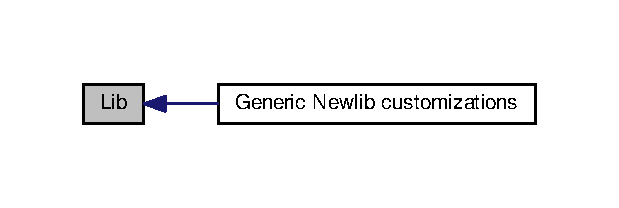
\includegraphics[width=297pt]{group__lib}
\end{center}
\end{figure}
\subsection*{Módulos}
\begin{DoxyCompactItemize}
\item 
\hyperlink{group__newlib}{Generic Newlib customizations}
\begin{DoxyCompactList}\small\item\em Library providing generic implementations of Newlib features for Contiki. \end{DoxyCompactList}\end{DoxyCompactItemize}


\subsection{Descrição detalhada}

\hypertarget{group__newlib}{\section{Generic Newlib customizations}
\label{group__newlib}\index{Generic Newlib customizations@{Generic Newlib customizations}}
}


Library providing generic implementations of Newlib features for Contiki.  


Diagrama de colaboração para Generic Newlib customizations\+:\nopagebreak
\begin{figure}[H]
\begin{center}
\leavevmode
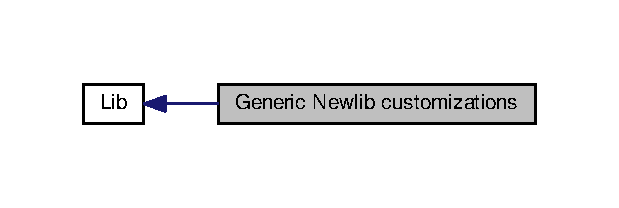
\includegraphics[width=297pt]{group__newlib}
\end{center}
\end{figure}
\subsection*{Ficheiros}
\begin{DoxyCompactItemize}
\item 
ficheiro \hyperlink{syscalls_8c}{syscalls.\+c}
\begin{DoxyCompactList}\small\item\em System calls. \end{DoxyCompactList}\end{DoxyCompactItemize}
\subsection*{Macros}
\begin{DoxyCompactItemize}
\item 
\hypertarget{group__newlib_gad72dbcf6d0153db1b8d8a58001feed83}{\#define {\bfseries D\+E\+B\+U\+G}~0}\label{group__newlib_gad72dbcf6d0153db1b8d8a58001feed83}

\item 
\hypertarget{group__newlib_ga1f464e950a4fa11e8821b5c725921a15}{\#define {\bfseries P\+R\+I\+N\+T\+F}(...)}\label{group__newlib_ga1f464e950a4fa11e8821b5c725921a15}

\end{DoxyCompactItemize}
\subsection*{Funções}
\begin{DoxyCompactItemize}
\item 
caddr\+\_\+t \hyperlink{group__newlib_gaae54d7b9578ba1fc171ce6f30f4c68a3}{\+\_\+sbrk} (int incr)
\begin{DoxyCompactList}\small\item\em Enlarges the allocated heap space. \end{DoxyCompactList}\end{DoxyCompactItemize}


\subsection{Descrição detalhada}
Library providing generic implementations of Newlib features for Contiki. 



\subsection{Documentação das funções}
\hypertarget{group__newlib_gaae54d7b9578ba1fc171ce6f30f4c68a3}{\index{Generic Newlib customizations@{Generic Newlib customizations}!\+\_\+sbrk@{\+\_\+sbrk}}
\index{\+\_\+sbrk@{\+\_\+sbrk}!Generic Newlib customizations@{Generic Newlib customizations}}
\subsubsection[{\+\_\+sbrk}]{\setlength{\rightskip}{0pt plus 5cm}caddr\+\_\+t \+\_\+sbrk (
\begin{DoxyParamCaption}
\item[{int}]{incr}
\end{DoxyParamCaption}
)}}\label{group__newlib_gaae54d7b9578ba1fc171ce6f30f4c68a3}


Enlarges the allocated heap space. 


\begin{DoxyParams}{Parâmetros}
{\em incr} & Number of bytes by which to increase the heap space \\
\hline
\end{DoxyParams}
\begin{DoxyReturn}{Retorna}
The previous end of heap on success (which is also a pointer to the start of the newly allocated memory if {\ttfamily incr} is positive), or {\ttfamily (caddr\+\_\+t)-\/1} with {\ttfamily errno} set to {\ttfamily E\+N\+O\+M\+E\+M} on error 
\end{DoxyReturn}

\begin{DoxyCode}
64 \{
65   \textcolor{comment}{/*}
66 \textcolor{comment}{   * Newlib's \_sbrk\_r() assumes that this global errno variable is used here,}
67 \textcolor{comment}{   * which is different from the errno definition provided by <errno.h>.}
68 \textcolor{comment}{   */}
69 \textcolor{preprocessor}{#undef errno}
70   \textcolor{keyword}{extern} \textcolor{keywordtype}{int} errno;
71 
72   \textcolor{comment}{/* Heap boundaries from linker script. */}
73   \textcolor{keyword}{extern} uint8\_t \_heap;
74   \textcolor{keyword}{extern} uint8\_t \_eheap;
75 
76   \textcolor{keyword}{static} uint8\_t *heap\_end = &\_heap;
77   uint8\_t *prev\_heap\_end = heap\_end;
78 
79   \textcolor{keywordflow}{if}(heap\_end + incr > &\_eheap) \{
80     PRINTF(\textcolor{stringliteral}{"Out of heap space!\(\backslash\)n"});
81     errno = ENOMEM;
82     \textcolor{keywordflow}{return} (caddr\_t)-1;
83   \}
84 
85   heap\_end += incr;
86   \textcolor{keywordflow}{return} (caddr\_t)prev\_heap\_end;
87 \}
\end{DoxyCode}

\chapter{Documentação da classe}
\hypertarget{structoid__data}{\section{Referência à estrutura oid\+\_\+data}
\label{structoid__data}\index{oid\+\_\+data@{oid\+\_\+data}}
}


Struct of O\+I\+D data in M\+I\+B Implementation.  




{\ttfamily \#include $<$mibii.\+h$>$}

\subsection*{Campos de Dados}
\begin{DoxyCompactItemize}
\item 
\hypertarget{structoid__data_a2675b7bf5cd84760d8e230b3f689d57d}{uint8\+\_\+t \hyperlink{structoid__data_a2675b7bf5cd84760d8e230b3f689d57d}{oid\+\_\+tree} \mbox{[}2\mbox{]}}\label{structoid__data_a2675b7bf5cd84760d8e230b3f689d57d}

\begin{DoxyCompactList}\small\item\em O\+I\+D tree value in the M\+I\+B. \end{DoxyCompactList}\item 
\hypertarget{structoid__data_a52f4f4b7f346c9d0a125c0cf2d934a73}{char \hyperlink{structoid__data_a52f4f4b7f346c9d0a125c0cf2d934a73}{oid\+\_\+value} \mbox{[}M\+A\+X\+\_\+\+S\+T\+R\+I\+N\+G\+S\+\_\+\+L\+E\+N\+G\+T\+H\mbox{]}}\label{structoid__data_a52f4f4b7f346c9d0a125c0cf2d934a73}

\begin{DoxyCompactList}\small\item\em O\+I\+D Data in the tree M\+I\+B Implementation. \end{DoxyCompactList}\end{DoxyCompactItemize}


\subsection{Descrição detalhada}
Struct of O\+I\+D data in M\+I\+B Implementation. 

A documentação para esta estrutura foi gerada a partir do seguinte ficheiro\+:\begin{DoxyCompactItemize}
\item 
snmpd/\hyperlink{mibii_8h}{mibii.\+h}\end{DoxyCompactItemize}

\hypertarget{structrequest}{\section{Referência à estrutura request}
\label{structrequest}\index{request@{request}}
}


Struct for request of S\+N\+M\+P Packets.  




{\ttfamily \#include $<$snmp.\+h$>$}



Diagrama de colaboração para request\+:\nopagebreak
\begin{figure}[H]
\begin{center}
\leavevmode
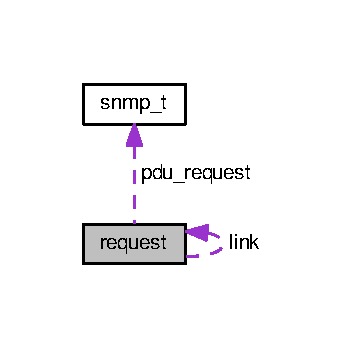
\includegraphics[width=166pt]{structrequest__coll__graph}
\end{center}
\end{figure}
\subsection*{Campos de Dados}
\begin{DoxyCompactItemize}
\item 
\hypertarget{structrequest_a445707e516f8c0aefe1ae30108d8e755}{\hyperlink{structsnmp__t}{snmp\+\_\+t} {\bfseries pdu\+\_\+request}}\label{structrequest_a445707e516f8c0aefe1ae30108d8e755}

\item 
\hypertarget{structrequest_acd3424c52c115fc00144c6679816c819}{struct \hyperlink{structrequest}{request} $\ast$ \hyperlink{structrequest_acd3424c52c115fc00144c6679816c819}{link}}\label{structrequest_acd3424c52c115fc00144c6679816c819}

\begin{DoxyCompactList}\small\item\em Link to the next request. \end{DoxyCompactList}\end{DoxyCompactItemize}


\subsection{Descrição detalhada}
Struct for request of S\+N\+M\+P Packets. 

A documentação para esta estrutura foi gerada a partir do seguinte ficheiro\+:\begin{DoxyCompactItemize}
\item 
snmpd/\hyperlink{snmp_8h}{snmp.\+h}\end{DoxyCompactItemize}

\hypertarget{structsnmp__con__t}{\section{Referência à estrutura snmp\+\_\+con\+\_\+t}
\label{structsnmp__con__t}\index{snmp\+\_\+con\+\_\+t@{snmp\+\_\+con\+\_\+t}}
}


Struct of S\+N\+M\+P Connection.  




{\ttfamily \#include $<$snmp.\+h$>$}



\subsection{Descrição detalhada}
Struct of S\+N\+M\+P Connection. 

A documentação para esta estrutura foi gerada a partir do seguinte ficheiro\+:\begin{DoxyCompactItemize}
\item 
snmpd/\hyperlink{snmp_8h}{snmp.\+h}\end{DoxyCompactItemize}

\hypertarget{structsnmp__t}{\section{Referência à estrutura snmp\+\_\+t}
\label{structsnmp__t}\index{snmp\+\_\+t@{snmp\+\_\+t}}
}


Struct for the S\+N\+M\+P Message.  




{\ttfamily \#include $<$snmp.\+h$>$}

\subsection*{Campos de Dados}
\begin{DoxyCompactItemize}
\item 
\hypertarget{structsnmp__t_a593b834134e4656a593ae9cf1ce6d201}{uint32\+\_\+t {\bfseries snmp\+\_\+version}}\label{structsnmp__t_a593b834134e4656a593ae9cf1ce6d201}

\item 
\hypertarget{structsnmp__t_acccc7895ee6181a7b3a1e15712402b55}{uint8\+\_\+t {\bfseries request\+\_\+type}}\label{structsnmp__t_acccc7895ee6181a7b3a1e15712402b55}

\item 
\hypertarget{structsnmp__t_a8ddc80b9c7bdb968e936f67c1cb61b41}{uint8\+\_\+t {\bfseries response\+\_\+type}}\label{structsnmp__t_a8ddc80b9c7bdb968e936f67c1cb61b41}

\item 
\hypertarget{structsnmp__t_a42b0bcd073d9adc8bf3e0045c3064fda}{uint8\+\_\+t {\bfseries request\+\_\+id\+\_\+c} \mbox{[}10\mbox{]}}\label{structsnmp__t_a42b0bcd073d9adc8bf3e0045c3064fda}

\item 
\hypertarget{structsnmp__t_a043bf20b6c2e89ee1df4fcc94072448d}{uint8\+\_\+t {\bfseries community} \mbox{[}\hyperlink{snmp_8h_a23bdc4d15d908a80e4bc06be55463ffc}{M\+A\+X\+\_\+\+O\+C\+T\+E\+T\+\_\+\+S\+T\+R\+I\+N\+G}\mbox{]}}\label{structsnmp__t_a043bf20b6c2e89ee1df4fcc94072448d}

\item 
\hypertarget{structsnmp__t_ab9c54bd7b1b1cffb109e66a9b3f82230}{uint8\+\_\+t {\bfseries oid\+\_\+encoded} \mbox{[}M\+A\+X\+\_\+\+O\+I\+D\+\_\+\+S\+T\+R\+I\+N\+G\mbox{]}}\label{structsnmp__t_ab9c54bd7b1b1cffb109e66a9b3f82230}

\item 
\hypertarget{structsnmp__t_a8e545ad997d63132958e084ada9ad750}{uint8\+\_\+t {\bfseries value} \mbox{[}\hyperlink{snmp_8h_a23bdc4d15d908a80e4bc06be55463ffc}{M\+A\+X\+\_\+\+O\+C\+T\+E\+T\+\_\+\+S\+T\+R\+I\+N\+G}\mbox{]}}\label{structsnmp__t_a8e545ad997d63132958e084ada9ad750}

\end{DoxyCompactItemize}


\subsection{Descrição detalhada}
Struct for the S\+N\+M\+P Message. 

A documentação para esta estrutura foi gerada a partir do seguinte ficheiro\+:\begin{DoxyCompactItemize}
\item 
snmpd/\hyperlink{snmp_8h}{snmp.\+h}\end{DoxyCompactItemize}

\chapter{Documentação do ficheiro}
\hypertarget{homestark_8h}{\section{Referência ao ficheiro homestark.\+h}
\label{homestark_8h}\index{homestark.\+h@{homestark.\+h}}
}


Licensed to the Apache Software Foundation (A\+S\+F) under one or more contributor license agreements.  


Este grafo mostra quais são os ficheiros que incluem directamente ou indirectamente este ficheiro\+:\nopagebreak
\begin{figure}[H]
\begin{center}
\leavevmode
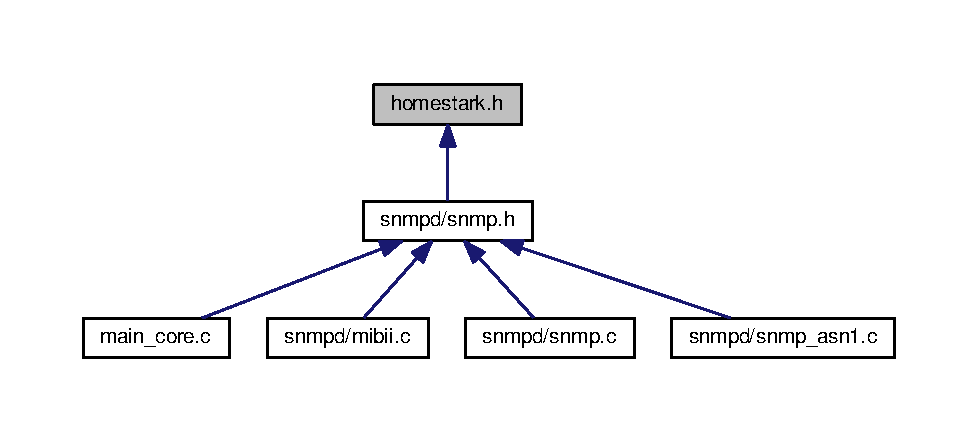
\includegraphics[width=350pt]{homestark_8h__dep__incl}
\end{center}
\end{figure}
\subsection*{Macros}
\begin{DoxyCompactItemize}
\item 
\hypertarget{homestark_8h_a7871b41b94f3b5aac9e79ad353903ae7}{\#define {\bfseries D\+E\+B\+U\+G\+\_\+\+O\+S}}\label{homestark_8h_a7871b41b94f3b5aac9e79ad353903ae7}

\item 
\hypertarget{homestark_8h_a4414818dcd874c17a091c7a4d9f9ed37}{\#define {\bfseries debug\+\_\+os}(fmt, args...)~printf(\char`\"{}\textbackslash{}n\mbox{[}Home\+Stark\mbox{]} \char`\"{}fmt, \#\#args)}\label{homestark_8h_a4414818dcd874c17a091c7a4d9f9ed37}

\item 
\hypertarget{homestark_8h_aa3d71c2e4384176175dd39591eaa85eb}{\#define {\bfseries D\+E\+B\+U\+G\+\_\+\+C\+O\+A\+P}}\label{homestark_8h_aa3d71c2e4384176175dd39591eaa85eb}

\item 
\hypertarget{homestark_8h_a64a3b6074452476fb66eb0314de522f5}{\#define {\bfseries debug\+\_\+coap}(fmt, args...)~printf(\char`\"{}\textbackslash{}n\mbox{[}Co\+A\+P\mbox{]} \char`\"{}fmt, \#\#args)}\label{homestark_8h_a64a3b6074452476fb66eb0314de522f5}

\end{DoxyCompactItemize}


\subsection{Descrição detalhada}
Licensed to the Apache Software Foundation (A\+S\+F) under one or more contributor license agreements. 

See the N\+O\+T\+I\+C\+E file distributed with this work for additional information regarding copyright ownership. The A\+S\+F licenses this file to you under the Apache License, Version 2.\+0 (the \char`\"{}\+License\char`\"{}); you may not use this file except in compliance with the License. You may obtain a copy of the License at

\href{http://www.apache.org/licenses/LICENSE-2.0}{\tt http\+://www.\+apache.\+org/licenses/\+L\+I\+C\+E\+N\+S\+E-\/2.\+0}

Unless required by applicable law or agreed to in writing, software distributed under the License is distributed on an \char`\"{}\+A\+S I\+S\char`\"{} B\+A\+S\+I\+S, W\+I\+T\+H\+O\+U\+T W\+A\+R\+R\+A\+N\+T\+I\+E\+S O\+R C\+O\+N\+D\+I\+T\+I\+O\+N\+S O\+F A\+N\+Y K\+I\+N\+D, either express or implied. See the License for the specific language governing permissions and limitations under the License.

Este projeto está sendo liberado pela licença A\+P\+A\+C\+H\+E 2.\+0.

Conjunto de protótipos e definiçoes de funções utilizadas \begin{DoxyAuthor}{Autor}
Ânderson Ignácio da Silva 
\end{DoxyAuthor}
\begin{DoxyDate}{Data}
08 Set 2016 
\end{DoxyDate}
\begin{DoxySeeAlso}{Veja também}
\href{http://www.aignacio.com}{\tt http\+://www.\+aignacio.\+com} 
\end{DoxySeeAlso}

\hypertarget{main__core_8c}{\section{Referência ao ficheiro main\+\_\+core.\+c}
\label{main__core_8c}\index{main\+\_\+core.\+c@{main\+\_\+core.\+c}}
}


Arquivo principal do código fonte da rede mesh 6\+Lo\+W\+P\+A\+N ~\newline
 Para compilar este código, execute o makefile com o target desejado, por exemplo\+: ~\newline
 {\bfseries \char`\"{}make T\+A\+R\+G\+E\+T=srf06-\/cc26xx\char`\"{}} ~\newline
 Caso não reconheça qual o T\+A\+R\+G\+E\+T correto, utiliza o comando ~\newline
 {\bfseries \char`\"{}make targets\char`\"{}} ~\newline
 para listar os tags disponíveis.  


{\ttfamily \#include \char`\"{}contiki.\+h\char`\"{}}\\*
{\ttfamily \#include \char`\"{}lib/random.\+h\char`\"{}}\\*
{\ttfamily \#include \char`\"{}clock.\+h\char`\"{}}\\*
{\ttfamily \#include \char`\"{}sys/ctimer.\+h\char`\"{}}\\*
{\ttfamily \#include \char`\"{}net/ip/uip.\+h\char`\"{}}\\*
{\ttfamily \#include \char`\"{}net/ipv6/uip-\/ds6.\+h\char`\"{}}\\*
{\ttfamily \#include \char`\"{}mqtt\+\_\+sn.\+h\char`\"{}}\\*
{\ttfamily \#include \char`\"{}dev/leds.\+h\char`\"{}}\\*
{\ttfamily \#include \char`\"{}net/rime/rime.\+h\char`\"{}}\\*
{\ttfamily \#include \char`\"{}simple-\/udp.\+h\char`\"{}}\\*
{\ttfamily \#include $<$stdio.\+h$>$}\\*
{\ttfamily \#include $<$string.\+h$>$}\\*
{\ttfamily \#include $<$stdlib.\+h$>$}\\*
Diagrama de dependências de inclusão para main\+\_\+core.\+c\+:\nopagebreak
\begin{figure}[H]
\begin{center}
\leavevmode
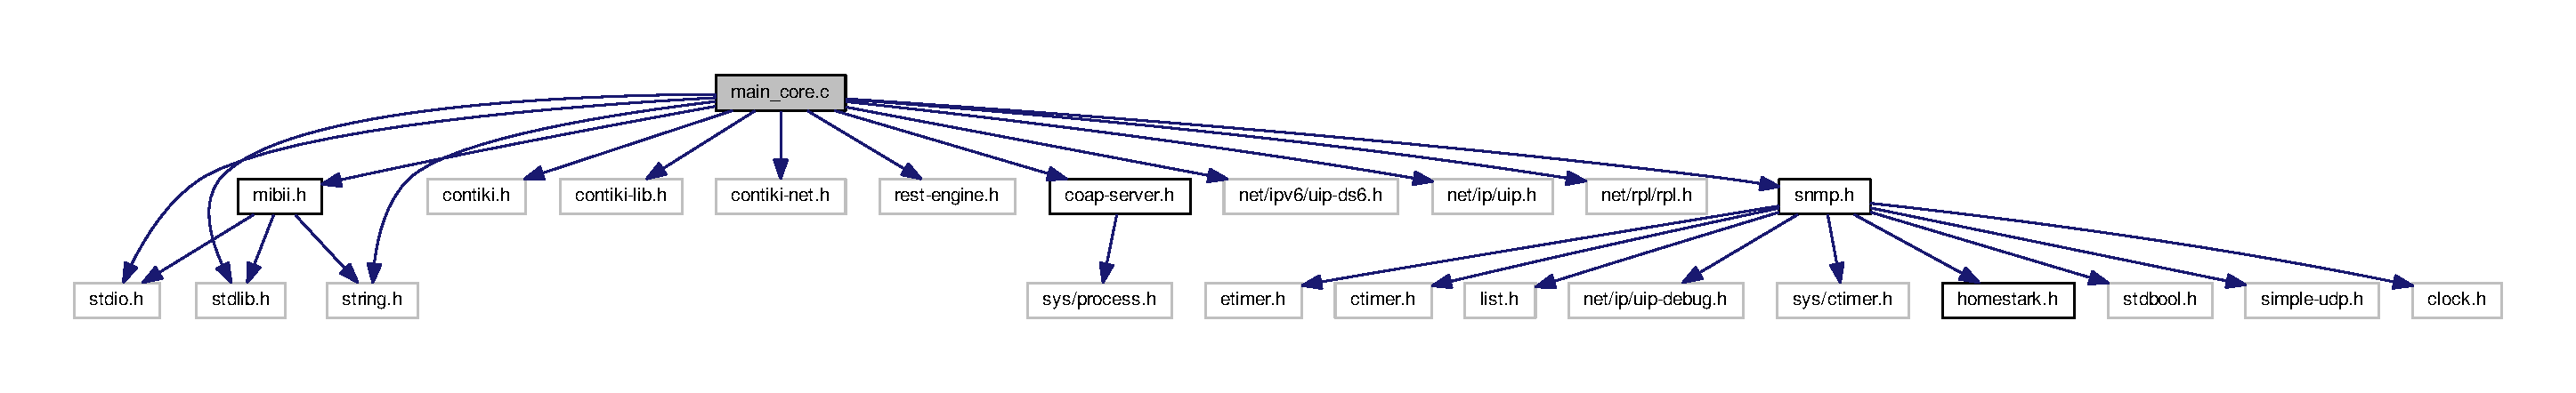
\includegraphics[width=350pt]{main__core_8c__incl}
\end{center}
\end{figure}
\subsection*{Funções}
\begin{DoxyCompactItemize}
\item 
\hypertarget{main__core_8c_a0a43995afea1479f111fbc2e35be0a7c}{void {\bfseries mqtt\+\_\+sn\+\_\+callback} (char $\ast$topic, char $\ast$message)}\label{main__core_8c_a0a43995afea1479f111fbc2e35be0a7c}

\item 
\hypertarget{main__core_8c_a271e0d9822452758a68f6e167c5209f8}{void {\bfseries init\+\_\+broker} (void)}\label{main__core_8c_a271e0d9822452758a68f6e167c5209f8}

\item 
\hypertarget{main__core_8c_a79354dfce54fd0bece29f8d443321b88}{{\bfseries P\+R\+O\+C\+E\+S\+S} (init\+\_\+system\+\_\+process,\char`\"{}\mbox{[}Contiki-\/O\+S\mbox{]} Iniciando sistema operacional\char`\"{})}\label{main__core_8c_a79354dfce54fd0bece29f8d443321b88}

\item 
\hypertarget{main__core_8c_a7683f5bdcb8cfbbb750ce92e76d1b7eb}{{\bfseries P\+R\+O\+C\+E\+S\+S\+\_\+\+T\+H\+R\+E\+A\+D} (init\+\_\+system\+\_\+process, ev, data)}\label{main__core_8c_a7683f5bdcb8cfbbb750ce92e76d1b7eb}

\end{DoxyCompactItemize}
\subsection*{Variáveis}
\begin{DoxyCompactItemize}
\item 
\hypertarget{main__core_8c_a5ca81254b9031056ba22742fb2252fd0}{\hyperlink{structmqtt__sn__con__t}{mqtt\+\_\+sn\+\_\+con\+\_\+t} {\bfseries mqtt\+\_\+sn\+\_\+connection}}\label{main__core_8c_a5ca81254b9031056ba22742fb2252fd0}

\item 
\hypertarget{main__core_8c_ac531a18312af7e29d65ccde0edd8b894}{A\+U\+T\+O\+S\+T\+A\+R\+T\+\_\+\+P\+R\+O\+C\+E\+S\+S\+E\+S \& {\bfseries init\+\_\+system\+\_\+process}}\label{main__core_8c_ac531a18312af7e29d65ccde0edd8b894}

\end{DoxyCompactItemize}


\subsection{Descrição detalhada}
Arquivo principal do código fonte da rede mesh 6\+Lo\+W\+P\+A\+N ~\newline
 Para compilar este código, execute o makefile com o target desejado, por exemplo\+: ~\newline
 {\bfseries \char`\"{}make T\+A\+R\+G\+E\+T=srf06-\/cc26xx\char`\"{}} ~\newline
 Caso não reconheça qual o T\+A\+R\+G\+E\+T correto, utiliza o comando ~\newline
 {\bfseries \char`\"{}make targets\char`\"{}} ~\newline
 para listar os tags disponíveis. 

\begin{DoxyAuthor}{Autor}
Ânderson Ignácio da Silva 
\end{DoxyAuthor}
\begin{DoxyDate}{Data}
19 Ago 2016 
\end{DoxyDate}
\begin{DoxySeeAlso}{Veja também}
\href{http://www.aignacio.com}{\tt http\+://www.\+aignacio.\+com} 
\end{DoxySeeAlso}

\hypertarget{project-conf_8h}{\section{Referência ao ficheiro project-\/conf.h}
\label{project-conf_8h}\index{project-\/conf.\+h@{project-\/conf.\+h}}
}


\begin{DoxyVerb} Erbium (Er) example project configuration.\end{DoxyVerb}
  


\subsection*{Macros}
\begin{DoxyCompactItemize}
\item 
\hypertarget{project-conf_8h_a713b73648671626232b7f8c3dca1d939}{\#define {\bfseries N\+E\+T\+S\+T\+A\+C\+K\+\_\+\+C\+O\+N\+F\+\_\+\+R\+D\+C}~contikimac\+\_\+driver}\label{project-conf_8h_a713b73648671626232b7f8c3dca1d939}

\item 
\hypertarget{project-conf_8h_aeb62bc51ff0305451eabedcc54a0fdfa}{\#define {\bfseries R\+P\+L\+\_\+\+C\+O\+N\+F\+\_\+\+M\+A\+X\+\_\+\+D\+A\+G\+\_\+\+P\+E\+R\+\_\+\+I\+N\+S\+T\+A\+N\+C\+E}~1}\label{project-conf_8h_aeb62bc51ff0305451eabedcc54a0fdfa}

\item 
\hypertarget{project-conf_8h_af040984efb79765f3079be76b7499168}{\#define {\bfseries U\+I\+P\+\_\+\+C\+O\+N\+F\+\_\+\+T\+C\+P}~0}\label{project-conf_8h_af040984efb79765f3079be76b7499168}

\item 
\hypertarget{project-conf_8h_a4be5f67e37edb6a213d34e8c1968544f}{\#define {\bfseries N\+E\+T\+S\+T\+A\+C\+K\+\_\+\+C\+O\+N\+F\+\_\+\+M\+A\+C}~nullmac\+\_\+driver}\label{project-conf_8h_a4be5f67e37edb6a213d34e8c1968544f}

\item 
\hypertarget{project-conf_8h_a9a3efae7c7faf00ea590ce25ba7eccc3}{\#define {\bfseries R\+E\+S\+T\+\_\+\+M\+A\+X\+\_\+\+C\+H\+U\+N\+K\+\_\+\+S\+I\+Z\+E}~48}\label{project-conf_8h_a9a3efae7c7faf00ea590ce25ba7eccc3}

\item 
\hypertarget{project-conf_8h_a47436509e3fc2f8dfbcbd463b0d97253}{\#define {\bfseries C\+O\+A\+P\+\_\+\+M\+A\+X\+\_\+\+O\+P\+E\+N\+\_\+\+T\+R\+A\+N\+S\+A\+C\+T\+I\+O\+N\+S}~4}\label{project-conf_8h_a47436509e3fc2f8dfbcbd463b0d97253}

\item 
\hypertarget{project-conf_8h_a89414d6478cb8ddbed6c1a44bb06014e}{\#define {\bfseries C\+O\+A\+P\+\_\+\+L\+I\+N\+K\+\_\+\+F\+O\+R\+M\+A\+T\+\_\+\+F\+I\+L\+T\+E\+R\+I\+N\+G}~0}\label{project-conf_8h_a89414d6478cb8ddbed6c1a44bb06014e}

\item 
\hypertarget{project-conf_8h_a70000cc8862dcde9bcf742f142a6e021}{\#define {\bfseries C\+O\+A\+P\+\_\+\+P\+R\+O\+X\+Y\+\_\+\+O\+P\+T\+I\+O\+N\+\_\+\+P\+R\+O\+C\+E\+S\+S\+I\+N\+G}~0}\label{project-conf_8h_a70000cc8862dcde9bcf742f142a6e021}

\item 
\hypertarget{project-conf_8h_aed383d82c438e6f6da89abb821dfc29c}{\#define {\bfseries R\+P\+L\+\_\+\+C\+O\+N\+F\+\_\+\+W\+I\+T\+H\+\_\+\+D\+A\+O\+\_\+\+A\+C\+K}~0}\label{project-conf_8h_aed383d82c438e6f6da89abb821dfc29c}

\item 
\hypertarget{project-conf_8h_a0c3bc93053ebf96d4b1daa2a9fb542a3}{\#define {\bfseries R\+P\+L\+\_\+\+C\+O\+N\+F\+\_\+\+O\+F}~rpl\+\_\+of0}\label{project-conf_8h_a0c3bc93053ebf96d4b1daa2a9fb542a3}

\item 
\hypertarget{project-conf_8h_a204fadd60d255b63620f1826bf030b60}{\#define {\bfseries C\+O\+A\+P\+\_\+\+O\+B\+S\+E\+R\+V\+E\+\_\+\+C\+L\+I\+E\+N\+T}~1}\label{project-conf_8h_a204fadd60d255b63620f1826bf030b60}

\end{DoxyCompactItemize}


\subsection{Descrição detalhada}
\begin{DoxyVerb} Erbium (Er) example project configuration.\end{DoxyVerb}
 

\begin{DoxyAuthor}{Autor}
Matthias Kovatsch \href{mailto:kovatsch@inf.ethz.ch}{\tt kovatsch@inf.\+ethz.\+ch} 
\end{DoxyAuthor}

\hypertarget{mibii_8c}{\section{Referência ao ficheiro snmpd/mibii.c}
\label{mibii_8c}\index{snmpd/mibii.\+c@{snmpd/mibii.\+c}}
}


Licensed to the Apache Software Foundation (A\+S\+F) under one or more contributor license agreements.  


{\ttfamily \#include $<$stdio.\+h$>$}\\*
{\ttfamily \#include $<$stdlib.\+h$>$}\\*
{\ttfamily \#include $<$string.\+h$>$}\\*
{\ttfamily \#include \char`\"{}snmp.\+h\char`\"{}}\\*
{\ttfamily \#include \char`\"{}mibii.\+h\char`\"{}}\\*
Diagrama de dependências de inclusão para mibii.\+c\+:\nopagebreak
\begin{figure}[H]
\begin{center}
\leavevmode
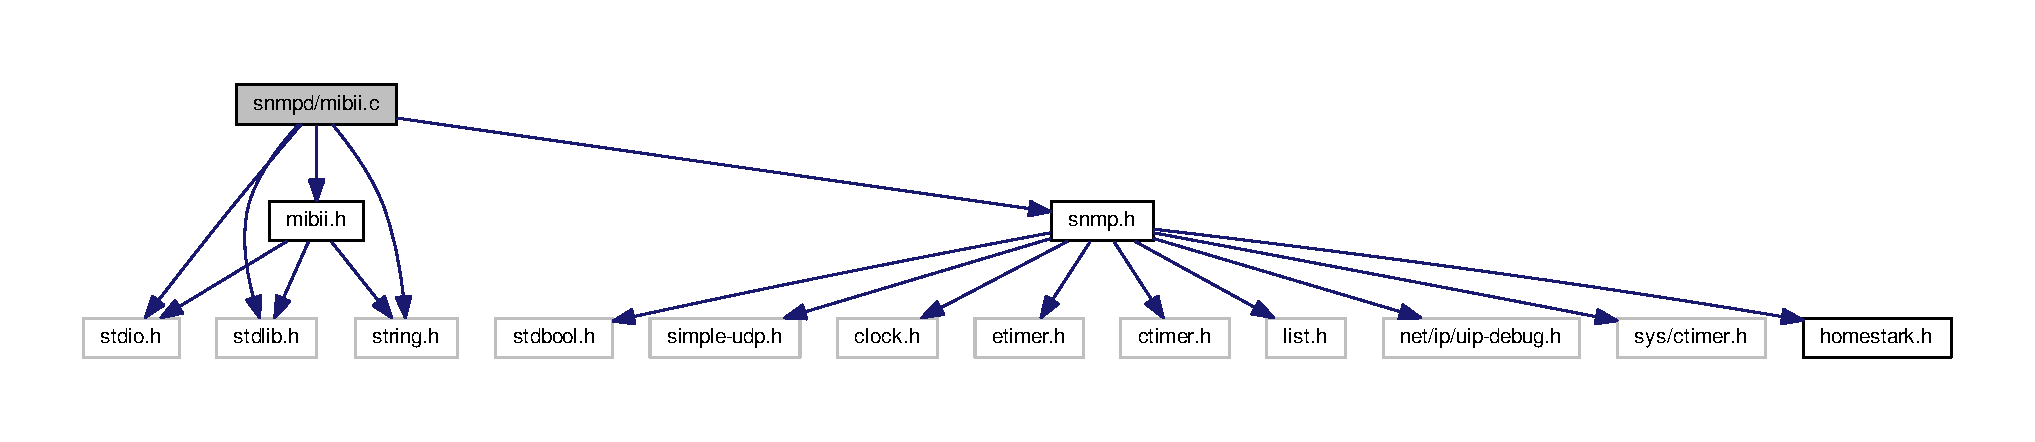
\includegraphics[width=350pt]{mibii_8c__incl}
\end{center}
\end{figure}
\subsection*{Funções}
\begin{DoxyCompactItemize}
\item 
\hyperlink{snmp_8h_add91ba4199db8665b9b9fc56fc6783a6}{resp\+\_\+con\+\_\+t} \hyperlink{mibii_8c_aeae05bfda8520c157c4436bc5cf8648b}{mib\+\_\+ii\+\_\+check\+\_\+oid} (uint8\+\_\+t $\ast$mib\+\_\+oid, uint8\+\_\+t $\ast$index)
\begin{DoxyCompactList}\small\item\em Check if exist O\+I\+D. \end{DoxyCompactList}\item 
\hyperlink{snmp_8h_add91ba4199db8665b9b9fc56fc6783a6}{resp\+\_\+con\+\_\+t} \hyperlink{mibii_8c_aa0bb802c0b80aaab6218e5a7753f8e28}{mib\+\_\+ii\+\_\+get\+\_\+oid} (uint8\+\_\+t $\ast$oid, uint8\+\_\+t $\ast$oid\+\_\+string)
\begin{DoxyCompactList}\small\item\em Get O\+I\+D Value in the M\+I\+B tree. \end{DoxyCompactList}\item 
\hyperlink{snmp_8h_add91ba4199db8665b9b9fc56fc6783a6}{resp\+\_\+con\+\_\+t} \hyperlink{mibii_8c_af534ed1c73b20f10d822d43da1ccc78e}{mib\+\_\+ii\+\_\+update\+\_\+list} (uint8\+\_\+t $\ast$tree, char $\ast$value)
\begin{DoxyCompactList}\small\item\em Update the M\+I\+B O\+I\+D Tree. \end{DoxyCompactList}\item 
\hyperlink{snmp_8h_add91ba4199db8665b9b9fc56fc6783a6}{resp\+\_\+con\+\_\+t} \hyperlink{mibii_8c_a87f7eaae8f191a87c287fc4896e3524e}{mib\+\_\+ii\+\_\+fill\+\_\+list} (uint8\+\_\+t $\ast$oid\+\_\+tree\+\_\+var, const char $\ast$value)
\begin{DoxyCompactList}\small\item\em Init the M\+I\+B O\+I\+D implementation. \end{DoxyCompactList}\item 
\hyperlink{snmp_8h_add91ba4199db8665b9b9fc56fc6783a6}{resp\+\_\+con\+\_\+t} \hyperlink{mibii_8c_a40c075666913ad4f73559ef972049d16}{mib\+\_\+ii\+\_\+show} (void)
\begin{DoxyCompactList}\small\item\em List M\+I\+B O\+I\+D values. \end{DoxyCompactList}\end{DoxyCompactItemize}
\subsection*{Variáveis}
\begin{DoxyCompactItemize}
\item 
\hypertarget{mibii_8c_a4d9874368b0a756022a37de20575c884}{uint8\+\_\+t {\bfseries global\+\_\+index} = 0}\label{mibii_8c_a4d9874368b0a756022a37de20575c884}

\item 
\hypertarget{mibii_8c_a8fe722bc2441f81a00d11912cf29126f}{\hyperlink{structoid__data}{oid\+\_\+data} {\bfseries oid\+\_\+list} \mbox{[}M\+A\+X\+\_\+\+O\+I\+D\+S\mbox{]}}\label{mibii_8c_a8fe722bc2441f81a00d11912cf29126f}

\end{DoxyCompactItemize}


\subsection{Descrição detalhada}
Licensed to the Apache Software Foundation (A\+S\+F) under one or more contributor license agreements. 

See the N\+O\+T\+I\+C\+E file distributed with this work for additional information regarding copyright ownership. The A\+S\+F licenses this file to you under the Apache License, Version 2.\+0 (the \char`\"{}\+License\char`\"{}); you may not use this file except in compliance with the License. You may obtain a copy of the License at

\href{http://www.apache.org/licenses/LICENSE-2.0}{\tt http\+://www.\+apache.\+org/licenses/\+L\+I\+C\+E\+N\+S\+E-\/2.\+0}

Unless required by applicable law or agreed to in writing, software distributed under the License is distributed on an \char`\"{}\+A\+S I\+S\char`\"{} B\+A\+S\+I\+S, W\+I\+T\+H\+O\+U\+T W\+A\+R\+R\+A\+N\+T\+I\+E\+S O\+R C\+O\+N\+D\+I\+T\+I\+O\+N\+S O\+F A\+N\+Y K\+I\+N\+D, either express or implied. See the License for the specific language governing permissions and limitations under the License.

This project is under A\+P\+A\+C\+H\+E 2.\+0 license.

M\+I\+B I\+I Implementation of homestark network \begin{DoxyAuthor}{Autor}
Ânderson Ignácio da Silva 
\end{DoxyAuthor}
\begin{DoxyDate}{Data}
19 Sept 2016 
\end{DoxyDate}
\begin{DoxySeeAlso}{Veja também}
\href{http://www.aignacio.com}{\tt http\+://www.\+aignacio.\+com} 
\end{DoxySeeAlso}


\subsection{Documentação das funções}
\hypertarget{mibii_8c_aeae05bfda8520c157c4436bc5cf8648b}{\index{mibii.\+c@{mibii.\+c}!mib\+\_\+ii\+\_\+check\+\_\+oid@{mib\+\_\+ii\+\_\+check\+\_\+oid}}
\index{mib\+\_\+ii\+\_\+check\+\_\+oid@{mib\+\_\+ii\+\_\+check\+\_\+oid}!mibii.\+c@{mibii.\+c}}
\subsubsection[{mib\+\_\+ii\+\_\+check\+\_\+oid}]{\setlength{\rightskip}{0pt plus 5cm}{\bf resp\+\_\+con\+\_\+t} mib\+\_\+ii\+\_\+check\+\_\+oid (
\begin{DoxyParamCaption}
\item[{uint8\+\_\+t $\ast$}]{mib\+\_\+oid, }
\item[{uint8\+\_\+t $\ast$}]{index}
\end{DoxyParamCaption}
)}}\label{mibii_8c_aeae05bfda8520c157c4436bc5cf8648b}


Check if exist O\+I\+D. 

Run in the M\+I\+B Structure to find O\+I\+D available.


\begin{DoxyParams}[1]{Parâmetros}
\mbox{\tt in}  & {\em mib\+\_\+oid} & O\+I\+D M\+I\+B tree string \\
\hline
\mbox{\tt in}  & {\em index} & Index of the position of the M\+I\+B searched\\
\hline
\end{DoxyParams}

\begin{DoxyRetVals}{Valores retornados}
{\em S\+U\+C\+C\+E\+S\+S\+\_\+\+C\+O\+N} & Success to find O\+I\+D value \\
\hline
{\em F\+A\+I\+L\+\_\+\+C\+O\+N} & Fail to find O\+I\+D value \\
\hline
\end{DoxyRetVals}

\begin{DoxyCode}
36                                                              \{
37   uint8\_t i,
38           mib\_s[4];
39   \textcolor{comment}{// A correct oid for this implementation must be iso.3.6.1.2.1.x.x.0}
40   mib\_s[0] = *(mib\_oid);
41   mib\_s[1] = *(mib\_oid+1),
42   mib\_s[2] = *(mib\_oid+2),
43   mib\_s[3] = *(mib\_oid+3);
44 
45 \textcolor{preprocessor}{  #ifdef DEBUG\_SNMP\_DECODING}
46   debug\_snmp(\textcolor{stringliteral}{"MIB to search: iso.3.6.1.2.1.[%d].[%d].[%d].[%d]"},mib\_s[0],mib\_s[1],mib\_s[2],mib\_s[3]);
47 \textcolor{preprocessor}{  #endif}
48 
49   \textcolor{keywordflow}{if} (mib\_s[2] != 0 || mib\_s[3] != 0)
50     \textcolor{keywordflow}{return} \hyperlink{snmp_8h_add91ba4199db8665b9b9fc56fc6783a6ac6ae922662cbaf7958eb387bfd6fe4da}{FAIL\_CON};
51 
52   \textcolor{keywordflow}{for} (i = 0; i < MAX\_OIDS; i++)\{
53     \textcolor{keywordflow}{if} (oid\_list[i].oid\_tree[0] == mib\_s[0] && oid\_list[i].oid\_tree[1] == mib\_s[1])\{
54       *index = i;
55       \textcolor{keywordflow}{return} \hyperlink{snmp_8h_add91ba4199db8665b9b9fc56fc6783a6ae7b7a388c90c2c5428cced225760885f}{SUCCESS\_CON};
56     \}
57     \textcolor{comment}{// debug\_snmp("%s",mibii\_tree[i]);}
58   \}
59 \textcolor{preprocessor}{  #ifdef DEBUG\_SNMP\_DECODING}
60   debug\_snmp(\textcolor{stringliteral}{"MIB2 - There isn't OID mapped!"});
61 \textcolor{preprocessor}{  #endif}
62   \textcolor{keywordflow}{return} \hyperlink{snmp_8h_add91ba4199db8665b9b9fc56fc6783a6ac6ae922662cbaf7958eb387bfd6fe4da}{FAIL\_CON};
63 \}
\end{DoxyCode}
\hypertarget{mibii_8c_a87f7eaae8f191a87c287fc4896e3524e}{\index{mibii.\+c@{mibii.\+c}!mib\+\_\+ii\+\_\+fill\+\_\+list@{mib\+\_\+ii\+\_\+fill\+\_\+list}}
\index{mib\+\_\+ii\+\_\+fill\+\_\+list@{mib\+\_\+ii\+\_\+fill\+\_\+list}!mibii.\+c@{mibii.\+c}}
\subsubsection[{mib\+\_\+ii\+\_\+fill\+\_\+list}]{\setlength{\rightskip}{0pt plus 5cm}{\bf resp\+\_\+con\+\_\+t} mib\+\_\+ii\+\_\+fill\+\_\+list (
\begin{DoxyParamCaption}
\item[{uint8\+\_\+t $\ast$}]{oid\+\_\+tree\+\_\+var, }
\item[{const char $\ast$}]{value}
\end{DoxyParamCaption}
)}}\label{mibii_8c_a87f7eaae8f191a87c287fc4896e3524e}


Init the M\+I\+B O\+I\+D implementation. 

Initialize the M\+I\+B O\+I\+D implementation structure


\begin{DoxyParams}[1]{Parâmetros}
\mbox{\tt in}  & {\em oid\+\_\+tree\+\_\+var} & O\+I\+D M\+I\+B tree string \\
\hline
\mbox{\tt in}  & {\em value} & Value to insert into O\+I\+D data\\
\hline
\end{DoxyParams}

\begin{DoxyRetVals}{Valores retornados}
{\em S\+U\+C\+C\+E\+S\+S\+\_\+\+C\+O\+N} & Success insert in the O\+I\+D M\+I\+B tree \\
\hline
{\em F\+A\+I\+L\+\_\+\+C\+O\+N} & Fail to insert in the O\+I\+D tree \\
\hline
\end{DoxyRetVals}

\begin{DoxyCode}
125                                                                      \{
126   \textcolor{keywordflow}{if} (global\_index == MAX\_OIDS) \textcolor{keywordflow}{return} \hyperlink{snmp_8h_add91ba4199db8665b9b9fc56fc6783a6ac6ae922662cbaf7958eb387bfd6fe4da}{FAIL\_CON};
127   uint8\_t index = global\_index++;
128 
129   oid\_list[index].\hyperlink{structoid__data_a2675b7bf5cd84760d8e230b3f689d57d}{oid\_tree}[0]  = *oid\_tree\_var;
130   oid\_list[index].\hyperlink{structoid__data_a2675b7bf5cd84760d8e230b3f689d57d}{oid\_tree}[1]  = *(oid\_tree\_var+1);
131   strcpy(oid\_list[index].oid\_value,value);
132 
133 
134   \textcolor{keywordflow}{return} \hyperlink{snmp_8h_add91ba4199db8665b9b9fc56fc6783a6ae7b7a388c90c2c5428cced225760885f}{SUCCESS\_CON};
135 \}
\end{DoxyCode}
\hypertarget{mibii_8c_aa0bb802c0b80aaab6218e5a7753f8e28}{\index{mibii.\+c@{mibii.\+c}!mib\+\_\+ii\+\_\+get\+\_\+oid@{mib\+\_\+ii\+\_\+get\+\_\+oid}}
\index{mib\+\_\+ii\+\_\+get\+\_\+oid@{mib\+\_\+ii\+\_\+get\+\_\+oid}!mibii.\+c@{mibii.\+c}}
\subsubsection[{mib\+\_\+ii\+\_\+get\+\_\+oid}]{\setlength{\rightskip}{0pt plus 5cm}{\bf resp\+\_\+con\+\_\+t} mib\+\_\+ii\+\_\+get\+\_\+oid (
\begin{DoxyParamCaption}
\item[{uint8\+\_\+t $\ast$}]{oid, }
\item[{uint8\+\_\+t $\ast$}]{oid\+\_\+string}
\end{DoxyParamCaption}
)}}\label{mibii_8c_aa0bb802c0b80aaab6218e5a7753f8e28}


Get O\+I\+D Value in the M\+I\+B tree. 

Search for O\+I\+D data in the M\+I\+B tree of the O\+I\+D passed.


\begin{DoxyParams}[1]{Parâmetros}
\mbox{\tt in}  & {\em oid} & O\+I\+D M\+I\+B tree string \\
\hline
\mbox{\tt in}  & {\em oid\+\_\+string} & String of the data in the O\+I\+D-\/\+M\+I\+B\\
\hline
\end{DoxyParams}

\begin{DoxyRetVals}{Valores retornados}
{\em S\+U\+C\+C\+E\+S\+S\+\_\+\+C\+O\+N} & Success to get the O\+I\+D Value \\
\hline
{\em F\+A\+I\+L\+\_\+\+C\+O\+N} & Fail to get the O\+I\+D Value \\
\hline
\end{DoxyRetVals}

\begin{DoxyCode}
65                                                             \{
66 \textcolor{preprocessor}{  #if CONTIKI\_TARGET\_SRF06\_CC26XX}
67     uint8\_t index;
68     \textcolor{keywordflow}{if} (!\hyperlink{mibii_8c_aeae05bfda8520c157c4436bc5cf8648b}{mib\_ii\_check\_oid}(oid+7,&index)) \textcolor{keywordflow}{return} \hyperlink{snmp_8h_add91ba4199db8665b9b9fc56fc6783a6ac6ae922662cbaf7958eb387bfd6fe4da}{FAIL\_CON};
69 
70     \textcolor{keywordtype}{char} data[MAX\_STRINGS\_LENGTH];
71     strcpy(data,oid\_list[index].oid\_value);
72 
73     uint8\_t len = strlen(data),
74             index2 = 0;
75     \textcolor{keywordflow}{while} (index2 <= len) \{
76       *(oid\_string+index2) = data[index2];
77       index2++;
78     \}
79     *(oid\_string+index2) = \textcolor{charliteral}{'\(\backslash\)0'};
80 
81 \textcolor{preprocessor}{    #ifdef DEBUG\_SNMP\_DECODING}
82     debug\_snmp(\textcolor{stringliteral}{"MIB2 Decode OID received:%s"},data);
83 \textcolor{preprocessor}{    #endif}
84     \textcolor{keywordflow}{return} \hyperlink{snmp_8h_add91ba4199db8665b9b9fc56fc6783a6ae7b7a388c90c2c5428cced225760885f}{SUCCESS\_CON};
85 \textcolor{preprocessor}{  #else}
86     uint8\_t data[] = \textcolor{stringliteral}{"z1\_snmp\(\backslash\)0"};
87     uint8\_t len = 8,
88             index2 = 0;
89     \textcolor{keywordflow}{while} (index2 <= len) \{
90       *(oid\_string+index2) = data[index2];
91       index2++;
92     \}
93     *(oid\_string+index2) = \textcolor{charliteral}{'\(\backslash\)0'};
94 \textcolor{preprocessor}{    #ifdef DEBUG\_SNMP\_DECODING}
95     debug\_snmp(\textcolor{stringliteral}{"MIB2 Decode OID received:%s"},(\textcolor{keywordtype}{char} *)oid\_string);
96 \textcolor{preprocessor}{    #endif}
97     \textcolor{keywordflow}{return} \hyperlink{snmp_8h_add91ba4199db8665b9b9fc56fc6783a6ae7b7a388c90c2c5428cced225760885f}{SUCCESS\_CON};
98 \textcolor{preprocessor}{  #endif}
99 \}
\end{DoxyCode}
\hypertarget{mibii_8c_a40c075666913ad4f73559ef972049d16}{\index{mibii.\+c@{mibii.\+c}!mib\+\_\+ii\+\_\+show@{mib\+\_\+ii\+\_\+show}}
\index{mib\+\_\+ii\+\_\+show@{mib\+\_\+ii\+\_\+show}!mibii.\+c@{mibii.\+c}}
\subsubsection[{mib\+\_\+ii\+\_\+show}]{\setlength{\rightskip}{0pt plus 5cm}{\bf resp\+\_\+con\+\_\+t} mib\+\_\+ii\+\_\+show (
\begin{DoxyParamCaption}
\item[{void}]{}
\end{DoxyParamCaption}
)}}\label{mibii_8c_a40c075666913ad4f73559ef972049d16}


List M\+I\+B O\+I\+D values. 

List all M\+I\+B Implementation with O\+I\+D tree and data


\begin{DoxyParams}[1]{Parâmetros}
\mbox{\tt in}  & {\em void} & Without argument\\
\hline
\end{DoxyParams}

\begin{DoxyRetVals}{Valores retornados}
{\em S\+U\+C\+C\+E\+S\+S\+\_\+\+C\+O\+N} & Success to list O\+I\+D tree \\
\hline
{\em F\+A\+I\+L\+\_\+\+C\+O\+N} & Fail to list O\+I\+D tree \\
\hline
\end{DoxyRetVals}

\begin{DoxyCode}
137                             \{
138   \textcolor{keywordtype}{size\_t} i = 0;
139 \textcolor{preprocessor}{  #ifdef DEBUG\_SNMP\_DECODING}
140     \textcolor{keywordflow}{for} (i=0; i < global\_index; i++) \{
141       debug\_snmp(\textcolor{stringliteral}{"Index:%d"},i);
142       debug\_snmp(\textcolor{stringliteral}{"OID Tree: iso.3.6.1.2.1.%d.%d.0"},oid\_list[i].oid\_tree[0],oid\_list[i].oid\_tree[1]);
143       debug\_snmp(\textcolor{stringliteral}{"OID Value:%s"},oid\_list[i].oid\_value);
144     \}
145 \textcolor{preprocessor}{  #endif}
146   \textcolor{keywordflow}{return} \hyperlink{snmp_8h_add91ba4199db8665b9b9fc56fc6783a6ae7b7a388c90c2c5428cced225760885f}{SUCCESS\_CON};
147 \}
\end{DoxyCode}
\hypertarget{mibii_8c_af534ed1c73b20f10d822d43da1ccc78e}{\index{mibii.\+c@{mibii.\+c}!mib\+\_\+ii\+\_\+update\+\_\+list@{mib\+\_\+ii\+\_\+update\+\_\+list}}
\index{mib\+\_\+ii\+\_\+update\+\_\+list@{mib\+\_\+ii\+\_\+update\+\_\+list}!mibii.\+c@{mibii.\+c}}
\subsubsection[{mib\+\_\+ii\+\_\+update\+\_\+list}]{\setlength{\rightskip}{0pt plus 5cm}{\bf resp\+\_\+con\+\_\+t} mib\+\_\+ii\+\_\+update\+\_\+list (
\begin{DoxyParamCaption}
\item[{uint8\+\_\+t $\ast$}]{tree, }
\item[{char $\ast$}]{value}
\end{DoxyParamCaption}
)}}\label{mibii_8c_af534ed1c73b20f10d822d43da1ccc78e}


Update the M\+I\+B O\+I\+D Tree. 

Search for O\+I\+D initialized and update the data in the tree


\begin{DoxyParams}[1]{Parâmetros}
\mbox{\tt in}  & {\em oid} & O\+I\+D M\+I\+B tree string \\
\hline
\mbox{\tt in}  & {\em oid\+\_\+string} & String of the data in the O\+I\+D-\/\+M\+I\+B\\
\hline
\end{DoxyParams}

\begin{DoxyRetVals}{Valores retornados}
{\em S\+U\+C\+C\+E\+S\+S\+\_\+\+C\+O\+N} & Success update the O\+I\+D M\+I\+B tree \\
\hline
{\em F\+A\+I\+L\+\_\+\+C\+O\+N} & Fail to update the O\+I\+D tree \\
\hline
\end{DoxyRetVals}

\begin{DoxyCode}
101                                                          \{
102   uint8\_t index\_list;
103   uint8\_t tree\_format[4];
104   uint8\_t mib1 = *tree;
105   uint8\_t mib2 = *(tree+1);
106 
107   tree\_format[0] = mib1;
108   tree\_format[1] = mib2;
109   tree\_format[2] = 0;
110   tree\_format[3] = 0;
111 
112   \textcolor{comment}{// sprintf((void *)tree\_format,"%c%c%c%c",mib1,mib2,mib3-0x30,mib4-0x30);}
113   \textcolor{keywordflow}{if} (!\hyperlink{mibii_8c_aeae05bfda8520c157c4436bc5cf8648b}{mib\_ii\_check\_oid}(tree\_format, &index\_list)) \textcolor{keywordflow}{return} 
      \hyperlink{snmp_8h_add91ba4199db8665b9b9fc56fc6783a6ac6ae922662cbaf7958eb387bfd6fe4da}{FAIL\_CON};
114   sprintf(oid\_list[index\_list].oid\_value,\textcolor{stringliteral}{"%s"},value);
115 
116 
117 \textcolor{preprocessor}{  #ifdef DEBUG\_SNMP\_DECODING}
118   debug\_snmp(\textcolor{stringliteral}{"Update MIB2 Indice:%d"},index\_list);
119   debug\_snmp(\textcolor{stringliteral}{"OID Tree: iso.3.6.1.2.1.%d.%d.0"},oid\_list[index\_list].oid\_tree[0],oid\_list[index\_list].
      oid\_tree[1]);
120   debug\_snmp(\textcolor{stringliteral}{"OID Value:%s"},oid\_list[index\_list].oid\_value);
121 \textcolor{preprocessor}{  #endif}
122   \textcolor{keywordflow}{return} \hyperlink{snmp_8h_add91ba4199db8665b9b9fc56fc6783a6ae7b7a388c90c2c5428cced225760885f}{SUCCESS\_CON};
123 \}
\end{DoxyCode}

\hypertarget{mibii_8h}{\section{Referência ao ficheiro snmpd/mibii.h}
\label{mibii_8h}\index{snmpd/mibii.\+h@{snmpd/mibii.\+h}}
}


Licensed to the Apache Software Foundation (A\+S\+F) under one or more contributor license agreements.  


{\ttfamily \#include $<$stdio.\+h$>$}\\*
{\ttfamily \#include $<$stdlib.\+h$>$}\\*
{\ttfamily \#include $<$string.\+h$>$}\\*
Diagrama de dependências de inclusão para mibii.\+h\+:\nopagebreak
\begin{figure}[H]
\begin{center}
\leavevmode
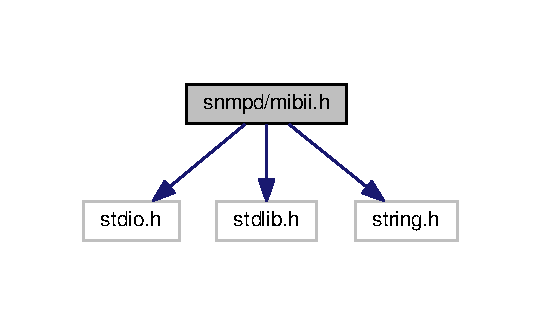
\includegraphics[width=260pt]{mibii_8h__incl}
\end{center}
\end{figure}
Este grafo mostra quais são os ficheiros que incluem directamente ou indirectamente este ficheiro\+:\nopagebreak
\begin{figure}[H]
\begin{center}
\leavevmode
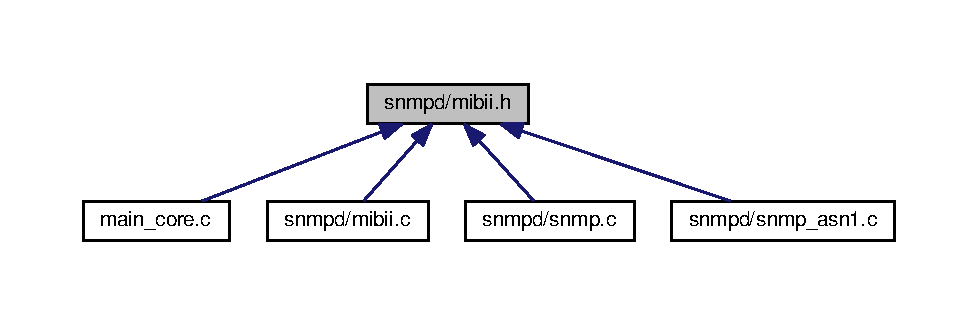
\includegraphics[width=350pt]{mibii_8h__dep__incl}
\end{center}
\end{figure}
\subsection*{Estruturas de Dados}
\begin{DoxyCompactItemize}
\item 
struct \hyperlink{structoid__data}{oid\+\_\+data}
\begin{DoxyCompactList}\small\item\em Struct of O\+I\+D data in M\+I\+B Implementation. \end{DoxyCompactList}\end{DoxyCompactItemize}
\subsection*{Funções}
\begin{DoxyCompactItemize}
\item 
\hyperlink{snmp_8h_add91ba4199db8665b9b9fc56fc6783a6}{resp\+\_\+con\+\_\+t} \hyperlink{mibii_8h_aeae05bfda8520c157c4436bc5cf8648b}{mib\+\_\+ii\+\_\+check\+\_\+oid} (uint8\+\_\+t $\ast$mib\+\_\+oid, uint8\+\_\+t $\ast$index)
\begin{DoxyCompactList}\small\item\em Check if exist O\+I\+D. \end{DoxyCompactList}\item 
\hyperlink{snmp_8h_add91ba4199db8665b9b9fc56fc6783a6}{resp\+\_\+con\+\_\+t} \hyperlink{mibii_8h_aa0bb802c0b80aaab6218e5a7753f8e28}{mib\+\_\+ii\+\_\+get\+\_\+oid} (uint8\+\_\+t $\ast$oid, uint8\+\_\+t $\ast$oid\+\_\+string)
\begin{DoxyCompactList}\small\item\em Get O\+I\+D Value in the M\+I\+B tree. \end{DoxyCompactList}\item 
\hyperlink{snmp_8h_add91ba4199db8665b9b9fc56fc6783a6}{resp\+\_\+con\+\_\+t} \hyperlink{mibii_8h_af534ed1c73b20f10d822d43da1ccc78e}{mib\+\_\+ii\+\_\+update\+\_\+list} (uint8\+\_\+t $\ast$tree, char $\ast$value)
\begin{DoxyCompactList}\small\item\em Update the M\+I\+B O\+I\+D Tree. \end{DoxyCompactList}\item 
\hyperlink{snmp_8h_add91ba4199db8665b9b9fc56fc6783a6}{resp\+\_\+con\+\_\+t} \hyperlink{mibii_8h_a87f7eaae8f191a87c287fc4896e3524e}{mib\+\_\+ii\+\_\+fill\+\_\+list} (uint8\+\_\+t $\ast$oid\+\_\+tree\+\_\+var, const char $\ast$value)
\begin{DoxyCompactList}\small\item\em Init the M\+I\+B O\+I\+D implementation. \end{DoxyCompactList}\item 
\hyperlink{snmp_8h_add91ba4199db8665b9b9fc56fc6783a6}{resp\+\_\+con\+\_\+t} \hyperlink{mibii_8h_a40c075666913ad4f73559ef972049d16}{mib\+\_\+ii\+\_\+show} (void)
\begin{DoxyCompactList}\small\item\em List M\+I\+B O\+I\+D values. \end{DoxyCompactList}\end{DoxyCompactItemize}


\subsection{Descrição detalhada}
Licensed to the Apache Software Foundation (A\+S\+F) under one or more contributor license agreements. 

See the N\+O\+T\+I\+C\+E file distributed with this work for additional information regarding copyright ownership. The A\+S\+F licenses this file to you under the Apache License, Version 2.\+0 (the \char`\"{}\+License\char`\"{}); you may not use this file except in compliance with the License. You may obtain a copy of the License at

\href{http://www.apache.org/licenses/LICENSE-2.0}{\tt http\+://www.\+apache.\+org/licenses/\+L\+I\+C\+E\+N\+S\+E-\/2.\+0}

Unless required by applicable law or agreed to in writing, software distributed under the License is distributed on an \char`\"{}\+A\+S I\+S\char`\"{} B\+A\+S\+I\+S, W\+I\+T\+H\+O\+U\+T W\+A\+R\+R\+A\+N\+T\+I\+E\+S O\+R C\+O\+N\+D\+I\+T\+I\+O\+N\+S O\+F A\+N\+Y K\+I\+N\+D, either express or implied. See the License for the specific language governing permissions and limitations under the License.

This project is under A\+P\+A\+C\+H\+E 2.\+0 license.

M\+I\+B I\+I Headers and definitions \begin{DoxyAuthor}{Autor}
Ânderson Ignácio da Silva 
\end{DoxyAuthor}
\begin{DoxyDate}{Data}
19 Sept 2016 
\end{DoxyDate}
\begin{DoxySeeAlso}{Veja também}
\href{http://www.aignacio.com}{\tt http\+://www.\+aignacio.\+com} 
\end{DoxySeeAlso}


\subsection{Documentação das funções}
\hypertarget{mibii_8h_aeae05bfda8520c157c4436bc5cf8648b}{\index{mibii.\+h@{mibii.\+h}!mib\+\_\+ii\+\_\+check\+\_\+oid@{mib\+\_\+ii\+\_\+check\+\_\+oid}}
\index{mib\+\_\+ii\+\_\+check\+\_\+oid@{mib\+\_\+ii\+\_\+check\+\_\+oid}!mibii.\+h@{mibii.\+h}}
\subsubsection[{mib\+\_\+ii\+\_\+check\+\_\+oid}]{\setlength{\rightskip}{0pt plus 5cm}{\bf resp\+\_\+con\+\_\+t} mib\+\_\+ii\+\_\+check\+\_\+oid (
\begin{DoxyParamCaption}
\item[{uint8\+\_\+t $\ast$}]{mib\+\_\+oid, }
\item[{uint8\+\_\+t $\ast$}]{index}
\end{DoxyParamCaption}
)}}\label{mibii_8h_aeae05bfda8520c157c4436bc5cf8648b}


Check if exist O\+I\+D. 

Run in the M\+I\+B Structure to find O\+I\+D available.


\begin{DoxyParams}[1]{Parâmetros}
\mbox{\tt in}  & {\em mib\+\_\+oid} & O\+I\+D M\+I\+B tree string \\
\hline
\mbox{\tt in}  & {\em index} & Index of the position of the M\+I\+B searched\\
\hline
\end{DoxyParams}

\begin{DoxyRetVals}{Valores retornados}
{\em S\+U\+C\+C\+E\+S\+S\+\_\+\+C\+O\+N} & Success to find O\+I\+D value \\
\hline
{\em F\+A\+I\+L\+\_\+\+C\+O\+N} & Fail to find O\+I\+D value \\
\hline
\end{DoxyRetVals}

\begin{DoxyCode}
36                                                              \{
37   uint8\_t i,
38           mib\_s[4];
39   \textcolor{comment}{// A correct oid for this implementation must be iso.3.6.1.2.1.x.x.0}
40   mib\_s[0] = *(mib\_oid);
41   mib\_s[1] = *(mib\_oid+1),
42   mib\_s[2] = *(mib\_oid+2),
43   mib\_s[3] = *(mib\_oid+3);
44 
45 \textcolor{preprocessor}{  #ifdef DEBUG\_SNMP\_DECODING}
46   debug\_snmp(\textcolor{stringliteral}{"MIB to search: iso.3.6.1.2.1.[%d].[%d].[%d].[%d]"},mib\_s[0],mib\_s[1],mib\_s[2],mib\_s[3]);
47 \textcolor{preprocessor}{  #endif}
48 
49   \textcolor{keywordflow}{if} (mib\_s[2] != 0 || mib\_s[3] != 0)
50     \textcolor{keywordflow}{return} \hyperlink{snmp_8h_add91ba4199db8665b9b9fc56fc6783a6ac6ae922662cbaf7958eb387bfd6fe4da}{FAIL\_CON};
51 
52   \textcolor{keywordflow}{for} (i = 0; i < MAX\_OIDS; i++)\{
53     \textcolor{keywordflow}{if} (oid\_list[i].oid\_tree[0] == mib\_s[0] && oid\_list[i].oid\_tree[1] == mib\_s[1])\{
54       *index = i;
55       \textcolor{keywordflow}{return} \hyperlink{snmp_8h_add91ba4199db8665b9b9fc56fc6783a6ae7b7a388c90c2c5428cced225760885f}{SUCCESS\_CON};
56     \}
57     \textcolor{comment}{// debug\_snmp("%s",mibii\_tree[i]);}
58   \}
59 \textcolor{preprocessor}{  #ifdef DEBUG\_SNMP\_DECODING}
60   debug\_snmp(\textcolor{stringliteral}{"MIB2 - There isn't OID mapped!"});
61 \textcolor{preprocessor}{  #endif}
62   \textcolor{keywordflow}{return} \hyperlink{snmp_8h_add91ba4199db8665b9b9fc56fc6783a6ac6ae922662cbaf7958eb387bfd6fe4da}{FAIL\_CON};
63 \}
\end{DoxyCode}
\hypertarget{mibii_8h_a87f7eaae8f191a87c287fc4896e3524e}{\index{mibii.\+h@{mibii.\+h}!mib\+\_\+ii\+\_\+fill\+\_\+list@{mib\+\_\+ii\+\_\+fill\+\_\+list}}
\index{mib\+\_\+ii\+\_\+fill\+\_\+list@{mib\+\_\+ii\+\_\+fill\+\_\+list}!mibii.\+h@{mibii.\+h}}
\subsubsection[{mib\+\_\+ii\+\_\+fill\+\_\+list}]{\setlength{\rightskip}{0pt plus 5cm}{\bf resp\+\_\+con\+\_\+t} mib\+\_\+ii\+\_\+fill\+\_\+list (
\begin{DoxyParamCaption}
\item[{uint8\+\_\+t $\ast$}]{oid\+\_\+tree\+\_\+var, }
\item[{const char $\ast$}]{value}
\end{DoxyParamCaption}
)}}\label{mibii_8h_a87f7eaae8f191a87c287fc4896e3524e}


Init the M\+I\+B O\+I\+D implementation. 

Initialize the M\+I\+B O\+I\+D implementation structure


\begin{DoxyParams}[1]{Parâmetros}
\mbox{\tt in}  & {\em oid\+\_\+tree\+\_\+var} & O\+I\+D M\+I\+B tree string \\
\hline
\mbox{\tt in}  & {\em value} & Value to insert into O\+I\+D data\\
\hline
\end{DoxyParams}

\begin{DoxyRetVals}{Valores retornados}
{\em S\+U\+C\+C\+E\+S\+S\+\_\+\+C\+O\+N} & Success insert in the O\+I\+D M\+I\+B tree \\
\hline
{\em F\+A\+I\+L\+\_\+\+C\+O\+N} & Fail to insert in the O\+I\+D tree \\
\hline
\end{DoxyRetVals}

\begin{DoxyCode}
125                                                                      \{
126   \textcolor{keywordflow}{if} (global\_index == MAX\_OIDS) \textcolor{keywordflow}{return} \hyperlink{snmp_8h_add91ba4199db8665b9b9fc56fc6783a6ac6ae922662cbaf7958eb387bfd6fe4da}{FAIL\_CON};
127   uint8\_t index = global\_index++;
128 
129   oid\_list[index].\hyperlink{structoid__data_a2675b7bf5cd84760d8e230b3f689d57d}{oid\_tree}[0]  = *oid\_tree\_var;
130   oid\_list[index].\hyperlink{structoid__data_a2675b7bf5cd84760d8e230b3f689d57d}{oid\_tree}[1]  = *(oid\_tree\_var+1);
131   strcpy(oid\_list[index].oid\_value,value);
132 
133 
134   \textcolor{keywordflow}{return} \hyperlink{snmp_8h_add91ba4199db8665b9b9fc56fc6783a6ae7b7a388c90c2c5428cced225760885f}{SUCCESS\_CON};
135 \}
\end{DoxyCode}
\hypertarget{mibii_8h_aa0bb802c0b80aaab6218e5a7753f8e28}{\index{mibii.\+h@{mibii.\+h}!mib\+\_\+ii\+\_\+get\+\_\+oid@{mib\+\_\+ii\+\_\+get\+\_\+oid}}
\index{mib\+\_\+ii\+\_\+get\+\_\+oid@{mib\+\_\+ii\+\_\+get\+\_\+oid}!mibii.\+h@{mibii.\+h}}
\subsubsection[{mib\+\_\+ii\+\_\+get\+\_\+oid}]{\setlength{\rightskip}{0pt plus 5cm}{\bf resp\+\_\+con\+\_\+t} mib\+\_\+ii\+\_\+get\+\_\+oid (
\begin{DoxyParamCaption}
\item[{uint8\+\_\+t $\ast$}]{oid, }
\item[{uint8\+\_\+t $\ast$}]{oid\+\_\+string}
\end{DoxyParamCaption}
)}}\label{mibii_8h_aa0bb802c0b80aaab6218e5a7753f8e28}


Get O\+I\+D Value in the M\+I\+B tree. 

Search for O\+I\+D data in the M\+I\+B tree of the O\+I\+D passed.


\begin{DoxyParams}[1]{Parâmetros}
\mbox{\tt in}  & {\em oid} & O\+I\+D M\+I\+B tree string \\
\hline
\mbox{\tt in}  & {\em oid\+\_\+string} & String of the data in the O\+I\+D-\/\+M\+I\+B\\
\hline
\end{DoxyParams}

\begin{DoxyRetVals}{Valores retornados}
{\em S\+U\+C\+C\+E\+S\+S\+\_\+\+C\+O\+N} & Success to get the O\+I\+D Value \\
\hline
{\em F\+A\+I\+L\+\_\+\+C\+O\+N} & Fail to get the O\+I\+D Value \\
\hline
\end{DoxyRetVals}

\begin{DoxyCode}
65                                                             \{
66 \textcolor{preprocessor}{  #if CONTIKI\_TARGET\_SRF06\_CC26XX}
67     uint8\_t index;
68     \textcolor{keywordflow}{if} (!\hyperlink{mibii_8c_aeae05bfda8520c157c4436bc5cf8648b}{mib\_ii\_check\_oid}(oid+7,&index)) \textcolor{keywordflow}{return} \hyperlink{snmp_8h_add91ba4199db8665b9b9fc56fc6783a6ac6ae922662cbaf7958eb387bfd6fe4da}{FAIL\_CON};
69 
70     \textcolor{keywordtype}{char} data[MAX\_STRINGS\_LENGTH];
71     strcpy(data,oid\_list[index].oid\_value);
72 
73     uint8\_t len = strlen(data),
74             index2 = 0;
75     \textcolor{keywordflow}{while} (index2 <= len) \{
76       *(oid\_string+index2) = data[index2];
77       index2++;
78     \}
79     *(oid\_string+index2) = \textcolor{charliteral}{'\(\backslash\)0'};
80 
81 \textcolor{preprocessor}{    #ifdef DEBUG\_SNMP\_DECODING}
82     debug\_snmp(\textcolor{stringliteral}{"MIB2 Decode OID received:%s"},data);
83 \textcolor{preprocessor}{    #endif}
84     \textcolor{keywordflow}{return} \hyperlink{snmp_8h_add91ba4199db8665b9b9fc56fc6783a6ae7b7a388c90c2c5428cced225760885f}{SUCCESS\_CON};
85 \textcolor{preprocessor}{  #else}
86     uint8\_t data[] = \textcolor{stringliteral}{"z1\_snmp\(\backslash\)0"};
87     uint8\_t len = 8,
88             index2 = 0;
89     \textcolor{keywordflow}{while} (index2 <= len) \{
90       *(oid\_string+index2) = data[index2];
91       index2++;
92     \}
93     *(oid\_string+index2) = \textcolor{charliteral}{'\(\backslash\)0'};
94 \textcolor{preprocessor}{    #ifdef DEBUG\_SNMP\_DECODING}
95     debug\_snmp(\textcolor{stringliteral}{"MIB2 Decode OID received:%s"},(\textcolor{keywordtype}{char} *)oid\_string);
96 \textcolor{preprocessor}{    #endif}
97     \textcolor{keywordflow}{return} \hyperlink{snmp_8h_add91ba4199db8665b9b9fc56fc6783a6ae7b7a388c90c2c5428cced225760885f}{SUCCESS\_CON};
98 \textcolor{preprocessor}{  #endif}
99 \}
\end{DoxyCode}
\hypertarget{mibii_8h_a40c075666913ad4f73559ef972049d16}{\index{mibii.\+h@{mibii.\+h}!mib\+\_\+ii\+\_\+show@{mib\+\_\+ii\+\_\+show}}
\index{mib\+\_\+ii\+\_\+show@{mib\+\_\+ii\+\_\+show}!mibii.\+h@{mibii.\+h}}
\subsubsection[{mib\+\_\+ii\+\_\+show}]{\setlength{\rightskip}{0pt plus 5cm}{\bf resp\+\_\+con\+\_\+t} mib\+\_\+ii\+\_\+show (
\begin{DoxyParamCaption}
\item[{void}]{}
\end{DoxyParamCaption}
)}}\label{mibii_8h_a40c075666913ad4f73559ef972049d16}


List M\+I\+B O\+I\+D values. 

List all M\+I\+B Implementation with O\+I\+D tree and data


\begin{DoxyParams}[1]{Parâmetros}
\mbox{\tt in}  & {\em void} & Without argument\\
\hline
\end{DoxyParams}

\begin{DoxyRetVals}{Valores retornados}
{\em S\+U\+C\+C\+E\+S\+S\+\_\+\+C\+O\+N} & Success to list O\+I\+D tree \\
\hline
{\em F\+A\+I\+L\+\_\+\+C\+O\+N} & Fail to list O\+I\+D tree \\
\hline
\end{DoxyRetVals}

\begin{DoxyCode}
137                             \{
138 \textcolor{preprocessor}{  #ifdef DEBUG\_SNMP\_DECODING}
139   \textcolor{keywordtype}{size\_t} i = 0;
140     \textcolor{keywordflow}{for} (i=0; i < global\_index; i++) \{
141       debug\_snmp(\textcolor{stringliteral}{"Index:%d"},i);
142       debug\_snmp(\textcolor{stringliteral}{"OID Tree: iso.3.6.1.2.1.%d.%d.0"},oid\_list[i].oid\_tree[0],oid\_list[i].oid\_tree[1]);
143       debug\_snmp(\textcolor{stringliteral}{"OID Value:%s"},oid\_list[i].oid\_value);
144     \}
145 \textcolor{preprocessor}{  #endif}
146   \textcolor{keywordflow}{return} \hyperlink{snmp_8h_add91ba4199db8665b9b9fc56fc6783a6ae7b7a388c90c2c5428cced225760885f}{SUCCESS\_CON};
147 \}
\end{DoxyCode}
\hypertarget{mibii_8h_af534ed1c73b20f10d822d43da1ccc78e}{\index{mibii.\+h@{mibii.\+h}!mib\+\_\+ii\+\_\+update\+\_\+list@{mib\+\_\+ii\+\_\+update\+\_\+list}}
\index{mib\+\_\+ii\+\_\+update\+\_\+list@{mib\+\_\+ii\+\_\+update\+\_\+list}!mibii.\+h@{mibii.\+h}}
\subsubsection[{mib\+\_\+ii\+\_\+update\+\_\+list}]{\setlength{\rightskip}{0pt plus 5cm}{\bf resp\+\_\+con\+\_\+t} mib\+\_\+ii\+\_\+update\+\_\+list (
\begin{DoxyParamCaption}
\item[{uint8\+\_\+t $\ast$}]{tree, }
\item[{char $\ast$}]{value}
\end{DoxyParamCaption}
)}}\label{mibii_8h_af534ed1c73b20f10d822d43da1ccc78e}


Update the M\+I\+B O\+I\+D Tree. 

Search for O\+I\+D initialized and update the data in the tree, we need to fill the O\+I\+D first


\begin{DoxyParams}[1]{Parâmetros}
\mbox{\tt in}  & {\em oid} & O\+I\+D M\+I\+B tree string \\
\hline
\mbox{\tt in}  & {\em oid\+\_\+string} & String of the data in the O\+I\+D-\/\+M\+I\+B\\
\hline
\end{DoxyParams}

\begin{DoxyRetVals}{Valores retornados}
{\em S\+U\+C\+C\+E\+S\+S\+\_\+\+C\+O\+N} & Success update the O\+I\+D M\+I\+B tree \\
\hline
{\em F\+A\+I\+L\+\_\+\+C\+O\+N} & Fail to update the O\+I\+D tree \\
\hline
\end{DoxyRetVals}

\begin{DoxyCode}
101                                                          \{
102   uint8\_t index\_list;
103   uint8\_t tree\_format[4];
104   uint8\_t mib1 = *tree;
105   uint8\_t mib2 = *(tree+1);
106 
107   tree\_format[0] = mib1;
108   tree\_format[1] = mib2;
109   tree\_format[2] = 0;
110   tree\_format[3] = 0;
111 
112   \textcolor{comment}{// sprintf((void *)tree\_format,"%c%c%c%c",mib1,mib2,mib3-0x30,mib4-0x30);}
113   \textcolor{keywordflow}{if} (!\hyperlink{mibii_8c_aeae05bfda8520c157c4436bc5cf8648b}{mib\_ii\_check\_oid}(tree\_format, &index\_list)) \textcolor{keywordflow}{return} 
      \hyperlink{snmp_8h_add91ba4199db8665b9b9fc56fc6783a6ac6ae922662cbaf7958eb387bfd6fe4da}{FAIL\_CON};
114   sprintf(oid\_list[index\_list].oid\_value,\textcolor{stringliteral}{"%s"},value);
115 
116 
117 \textcolor{preprocessor}{  #ifdef DEBUG\_SNMP\_DECODING}
118   debug\_snmp(\textcolor{stringliteral}{"Update MIB2 Indice:%d"},index\_list);
119   debug\_snmp(\textcolor{stringliteral}{"OID Tree: iso.3.6.1.2.1.%d.%d.0"},oid\_list[index\_list].oid\_tree[0],oid\_list[index\_list].
      oid\_tree[1]);
120   debug\_snmp(\textcolor{stringliteral}{"OID Value:%s"},oid\_list[index\_list].oid\_value);
121 \textcolor{preprocessor}{  #endif}
122   \textcolor{keywordflow}{return} \hyperlink{snmp_8h_add91ba4199db8665b9b9fc56fc6783a6ae7b7a388c90c2c5428cced225760885f}{SUCCESS\_CON};
123 \}
\end{DoxyCode}

\hypertarget{snmp_8c}{\section{Referência ao ficheiro snmpd/snmp.c}
\label{snmp_8c}\index{snmpd/snmp.\+c@{snmpd/snmp.\+c}}
}


Licensed to the Apache Software Foundation (A\+S\+F) under one or more contributor license agreements.  


{\ttfamily \#include $<$stdio.\+h$>$}\\*
{\ttfamily \#include $<$string.\+h$>$}\\*
{\ttfamily \#include $<$stdlib.\+h$>$}\\*
{\ttfamily \#include $<$stdint.\+h$>$}\\*
{\ttfamily \#include $<$stdbool.\+h$>$}\\*
{\ttfamily \#include $<$ctype.\+h$>$}\\*
{\ttfamily \#include \char`\"{}contiki.\+h\char`\"{}}\\*
{\ttfamily \#include \char`\"{}contiki-\/lib.\+h\char`\"{}}\\*
{\ttfamily \#include \char`\"{}contiki-\/net.\+h\char`\"{}}\\*
{\ttfamily \#include \char`\"{}snmp.\+h\char`\"{}}\\*
{\ttfamily \#include \char`\"{}mibii.\+h\char`\"{}}\\*
{\ttfamily \#include \char`\"{}net/rpl/rpl.\+h\char`\"{}}\\*
{\ttfamily \#include \char`\"{}net/ip/uip.\+h\char`\"{}}\\*
{\ttfamily \#include \char`\"{}net/ipv6/uip-\/ds6.\+h\char`\"{}}\\*
{\ttfamily \#include \char`\"{}simple-\/udp.\+h\char`\"{}}\\*
{\ttfamily \#include \char`\"{}list.\+h\char`\"{}}\\*
{\ttfamily \#include \char`\"{}sys/ctimer.\+h\char`\"{}}\\*
{\ttfamily \#include \char`\"{}sys/etimer.\+h\char`\"{}}\\*
{\ttfamily \#include \char`\"{}net/ip/uip-\/debug.\+h\char`\"{}}\\*
{\ttfamily \#include \char`\"{}net/rpl/rpl-\/private.\+h\char`\"{}}\\*
Diagrama de dependências de inclusão para snmp.\+c\+:\nopagebreak
\begin{figure}[H]
\begin{center}
\leavevmode
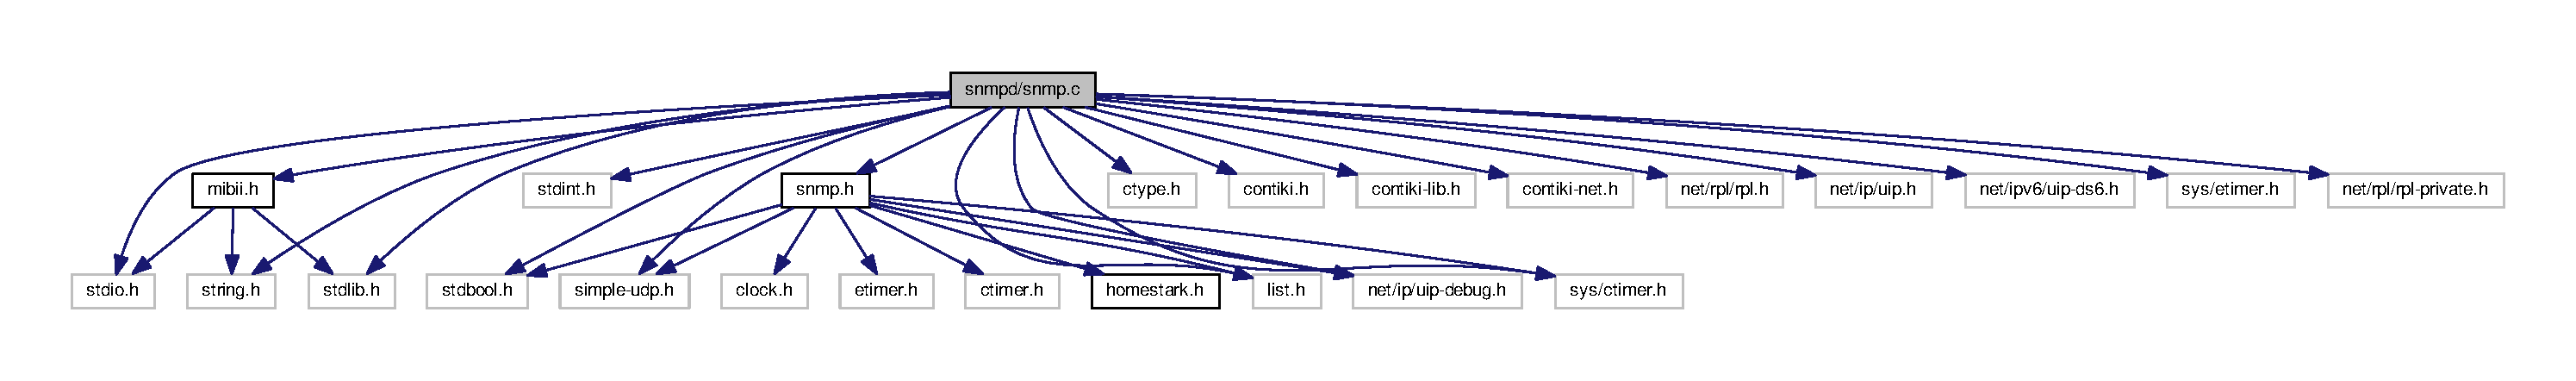
\includegraphics[width=350pt]{snmp_8c__incl}
\end{center}
\end{figure}
\subsection*{Macros}
\begin{DoxyCompactItemize}
\item 
\hypertarget{snmp_8c_af966537cf73ee5973da59bba6b21b731}{\#define {\bfseries U\+I\+P\+\_\+\+I\+P\+\_\+\+B\+U\+F}~((struct uip\+\_\+ip\+\_\+hdr $\ast$)\&uip\+\_\+buf\mbox{[}U\+I\+P\+\_\+\+L\+L\+H\+\_\+\+L\+E\+N\mbox{]})}\label{snmp_8c_af966537cf73ee5973da59bba6b21b731}

\item 
\hypertarget{snmp_8c_aaed757731852d359419ae5270a02e7a4}{\#define {\bfseries U\+I\+P\+\_\+\+U\+D\+P\+\_\+\+B\+U\+F}~((struct uip\+\_\+udp\+\_\+hdr $\ast$)\&uip\+\_\+buf\mbox{[}uip\+\_\+l2\+\_\+l3\+\_\+hdr\+\_\+len\mbox{]})}\label{snmp_8c_aaed757731852d359419ae5270a02e7a4}

\end{DoxyCompactItemize}
\subsection*{Funções}
\begin{DoxyCompactItemize}
\item 
\hypertarget{snmp_8c_a017be87c3d2f34ed9931125f00331652}{{\bfseries P\+R\+O\+C\+E\+S\+S} (snmp\+\_\+main,\char`\"{}\mbox{[}S\+N\+M\+P\mbox{]} S\+N\+M\+P\+D -\/ Agent V1\char`\"{})}\label{snmp_8c_a017be87c3d2f34ed9931125f00331652}

\item 
void \hyperlink{snmp_8c_a05848f4eb62dd417b99e461854870bf9}{snmp\+\_\+cb\+\_\+data} (void)
\begin{DoxyCompactList}\small\item\em S\+N\+M\+P Callback receive. \end{DoxyCompactList}\item 
void \hyperlink{snmp_8c_a4d88f2fc7655280384131d543e0d83e5}{snmp\+\_\+init} (void)
\begin{DoxyCompactList}\small\item\em S\+N\+M\+P Init function. \end{DoxyCompactList}\item 
int \hyperlink{snmp_8c_a523ab718dec1a794b3f8c8752f1e2ae3}{ipaddr\+\_\+sprintf} (char $\ast$buf, uint8\+\_\+t buf\+\_\+len, const uip\+\_\+ipaddr\+\_\+t $\ast$addr)
\begin{DoxyCompactList}\small\item\em Convert I\+Pv6 address in char format. \end{DoxyCompactList}\item 
void \hyperlink{snmp_8c_a732192a9e72d3182d395c47e2cd9c79e}{update\+\_\+snmp\+\_\+mib} (void)
\begin{DoxyCompactList}\small\item\em Update S\+N\+M\+P O\+I\+Ds. \end{DoxyCompactList}\item 
\hypertarget{snmp_8c_a06248b2be6d0f915906f3ac2a553a2c4}{{\bfseries P\+R\+O\+C\+E\+S\+S\+\_\+\+T\+H\+R\+E\+A\+D} (snmp\+\_\+main, ev, data)}\label{snmp_8c_a06248b2be6d0f915906f3ac2a553a2c4}

\end{DoxyCompactItemize}
\subsection*{Variáveis}
\begin{DoxyCompactItemize}
\item 
\hypertarget{snmp_8c_a46eb62b517b9cc09ba4cea868e920b12}{uint16\+\_\+t {\bfseries test} = 0}\label{snmp_8c_a46eb62b517b9cc09ba4cea868e920b12}

\end{DoxyCompactItemize}


\subsection{Descrição detalhada}
Licensed to the Apache Software Foundation (A\+S\+F) under one or more contributor license agreements. 

See the N\+O\+T\+I\+C\+E file distributed with this work for additional information regarding copyright ownership. The A\+S\+F licenses this file to you under the Apache License, Version 2.\+0 (the \char`\"{}\+License\char`\"{}); you may not use this file except in compliance with the License. You may obtain a copy of the License at

\href{http://www.apache.org/licenses/LICENSE-2.0}{\tt http\+://www.\+apache.\+org/licenses/\+L\+I\+C\+E\+N\+S\+E-\/2.\+0}

Unless required by applicable law or agreed to in writing, software distributed under the License is distributed on an \char`\"{}\+A\+S I\+S\char`\"{} B\+A\+S\+I\+S, W\+I\+T\+H\+O\+U\+T W\+A\+R\+R\+A\+N\+T\+I\+E\+S O\+R C\+O\+N\+D\+I\+T\+I\+O\+N\+S O\+F A\+N\+Y K\+I\+N\+D, either express or implied. See the License for the specific language governing permissions and limitations under the License.

This project is delivered under Apache 2.\+0 license.

Main functions of S\+N\+M\+P port \begin{DoxyAuthor}{Autor}
Ânderson Ignácio da Silva 
\end{DoxyAuthor}
\begin{DoxyDate}{Data}
12 Sept 2016 
\end{DoxyDate}
\begin{DoxySeeAlso}{Veja também}
\href{http://www.aignacio.com}{\tt http\+://www.\+aignacio.\+com} 
\end{DoxySeeAlso}


\subsection{Documentação das funções}
\hypertarget{snmp_8c_a523ab718dec1a794b3f8c8752f1e2ae3}{\index{snmp.\+c@{snmp.\+c}!ipaddr\+\_\+sprintf@{ipaddr\+\_\+sprintf}}
\index{ipaddr\+\_\+sprintf@{ipaddr\+\_\+sprintf}!snmp.\+c@{snmp.\+c}}
\subsubsection[{ipaddr\+\_\+sprintf}]{\setlength{\rightskip}{0pt plus 5cm}int ipaddr\+\_\+sprintf (
\begin{DoxyParamCaption}
\item[{char $\ast$}]{buf, }
\item[{uint8\+\_\+t}]{buf\+\_\+len, }
\item[{const uip\+\_\+ipaddr\+\_\+t $\ast$}]{addr}
\end{DoxyParamCaption}
)}}\label{snmp_8c_a523ab718dec1a794b3f8c8752f1e2ae3}


Convert I\+Pv6 address in char format. 

Format I\+Pv6 address in string char variable.


\begin{DoxyParams}[1]{Parâmetros}
\mbox{\tt in}  & {\em buf} & Variable that'll receive the ipv6 address decoded \\
\hline
\mbox{\tt in}  & {\em buf\+\_\+len} & Len of buf variable \\
\hline
\mbox{\tt in}  & {\em addr} & Address I\+Pv6 in uip\+\_\+ipaddr\+\_\+t format\\
\hline
\end{DoxyParams}

\begin{DoxyRetVals}{Valores retornados}
{\em len} & Length of buf variable formated \\
\hline
\end{DoxyRetVals}

\begin{DoxyCode}
101                                                                          \{
102   uint16\_t a;
103   uint8\_t len = 0;
104   \textcolor{keywordtype}{int} i, f;
105   \textcolor{keywordflow}{for}(i = 0, f = 0; i < \textcolor{keyword}{sizeof}(uip\_ipaddr\_t); i += 2) \{
106     a = (addr->u8[i] << 8) + addr->u8[i + 1];
107     \textcolor{keywordflow}{if}(a == 0 && f >= 0) \{
108       \textcolor{keywordflow}{if}(f++ == 0) \{
109         len += snprintf(&buf[len], buf\_len - len, \textcolor{stringliteral}{"::"});
110       \}
111     \} \textcolor{keywordflow}{else} \{
112       \textcolor{keywordflow}{if}(f > 0) \{
113         f = -1;
114       \} \textcolor{keywordflow}{else} \textcolor{keywordflow}{if}(i > 0) \{
115         len += snprintf(&buf[len], buf\_len - len, \textcolor{stringliteral}{":"});
116       \}
117       len += snprintf(&buf[len], buf\_len - len, \textcolor{stringliteral}{"%x"}, a);
118     \}
119   \}
120 
121   \textcolor{keywordflow}{return} len;
122 \}
\end{DoxyCode}
\hypertarget{snmp_8c_a05848f4eb62dd417b99e461854870bf9}{\index{snmp.\+c@{snmp.\+c}!snmp\+\_\+cb\+\_\+data@{snmp\+\_\+cb\+\_\+data}}
\index{snmp\+\_\+cb\+\_\+data@{snmp\+\_\+cb\+\_\+data}!snmp.\+c@{snmp.\+c}}
\subsubsection[{snmp\+\_\+cb\+\_\+data}]{\setlength{\rightskip}{0pt plus 5cm}void snmp\+\_\+cb\+\_\+data (
\begin{DoxyParamCaption}
\item[{void}]{}
\end{DoxyParamCaption}
)}}\label{snmp_8c_a05848f4eb62dd417b99e461854870bf9}


S\+N\+M\+P Callback receive. 

Receive in callback mode, any data from N\+M\+S of S\+N\+M\+P protocol.


\begin{DoxyParams}[1]{Parâmetros}
\mbox{\tt in}  & {\em void} & No argument to pass\\
\hline
\end{DoxyParams}

\begin{DoxyRetVals}{Valores retornados}
{\em void} & Doesn't return anything \\
\hline
\end{DoxyRetVals}

\begin{DoxyCode}
71                        \{
72   \textcolor{keyword}{static} uint16\_t len;
73   \textcolor{keyword}{static} \textcolor{keywordtype}{char} buf[MAX\_UDP\_SNMP];
74   memset(buf, 0, MAX\_UDP\_SNMP);
75 
76   \textcolor{keywordflow}{if}(uip\_newdata()) \{
77     len = uip\_datalen();
78     memcpy(buf, uip\_appdata, len);
79     debug\_snmp(\textcolor{stringliteral}{"%u bytes from ["}, len);
80     uip\_debug\_ipaddr\_print(&UIP\_IP\_BUF->srcipaddr);
81     printf(\textcolor{stringliteral}{"]:%u"}, UIP\_HTONS(UIP\_UDP\_BUF->srcport));
82     uip\_ipaddr\_copy(&server\_conn->ripaddr, &UIP\_IP\_BUF->srcipaddr);
83     server\_conn->rport = UIP\_UDP\_BUF->srcport;
84     \hyperlink{structsnmp__t}{snmp\_t} snmp\_handle;
85     \textcolor{keywordflow}{if} (\hyperlink{snmp_8h_aca484712bcdb0bbc0f065061c4a0ed20}{snmp\_decode\_message}(buf, &snmp\_handle))\{
86       debug\_snmp(\textcolor{stringliteral}{"New SNMP Request received!"});
87       len = \hyperlink{snmp_8h_a63d8ffecf9aa0af9824de046643c140f}{snmp\_encode\_message}(&snmp\_handle, buf);
88       uip\_udp\_packet\_send(server\_conn, buf, len);
89       uip\_create\_unspecified(&server\_conn->ripaddr);
90       server\_conn->rport = 0;
91     \}
92     \textcolor{keywordflow}{else}
93       debug\_snmp(\textcolor{stringliteral}{"Problem on SNMP Request received!"});
94   \}
95 \}
\end{DoxyCode}
\hypertarget{snmp_8c_a4d88f2fc7655280384131d543e0d83e5}{\index{snmp.\+c@{snmp.\+c}!snmp\+\_\+init@{snmp\+\_\+init}}
\index{snmp\+\_\+init@{snmp\+\_\+init}!snmp.\+c@{snmp.\+c}}
\subsubsection[{snmp\+\_\+init}]{\setlength{\rightskip}{0pt plus 5cm}void snmp\+\_\+init (
\begin{DoxyParamCaption}
\item[{void}]{}
\end{DoxyParamCaption}
)}}\label{snmp_8c_a4d88f2fc7655280384131d543e0d83e5}


S\+N\+M\+P Init function. 

Init S\+N\+M\+P A\+G\+E\+N\+T connection


\begin{DoxyParams}[1]{Parâmetros}
\mbox{\tt in}  & {\em void} & No argument to pass\\
\hline
\end{DoxyParams}

\begin{DoxyRetVals}{Valores retornados}
{\em void} & Not return argument \\
\hline
\end{DoxyRetVals}

\begin{DoxyCode}
97                     \{
98   process\_start(&snmp\_main, NULL);
99 \}
\end{DoxyCode}
\hypertarget{snmp_8c_a732192a9e72d3182d395c47e2cd9c79e}{\index{snmp.\+c@{snmp.\+c}!update\+\_\+snmp\+\_\+mib@{update\+\_\+snmp\+\_\+mib}}
\index{update\+\_\+snmp\+\_\+mib@{update\+\_\+snmp\+\_\+mib}!snmp.\+c@{snmp.\+c}}
\subsubsection[{update\+\_\+snmp\+\_\+mib}]{\setlength{\rightskip}{0pt plus 5cm}void update\+\_\+snmp\+\_\+mib (
\begin{DoxyParamCaption}
\item[{void}]{}
\end{DoxyParamCaption}
)}}\label{snmp_8c_a732192a9e72d3182d395c47e2cd9c79e}


Update S\+N\+M\+P O\+I\+Ds. 

Update the O\+I\+Ds of values from network


\begin{DoxyParams}[1]{Parâmetros}
\mbox{\tt in}  & {\em void} & No argument to pass\\
\hline
\end{DoxyParams}

\begin{DoxyRetVals}{Valores retornados}
{\em void} & Not return argument \\
\hline
\end{DoxyRetVals}

\begin{DoxyCode}
125                           \{
126   test++;
127 
128   uint8\_t oid\_tree[2];
129   \textcolor{keywordtype}{char} dado[MAX\_STRINGS\_LENGTH];
130 
131   \textcolor{comment}{/******************************* Hearbeat ***********************************/}
132   oid\_tree[0] = 4;
133   oid\_tree[1] = 1;
134   sprintf(dado,\textcolor{stringliteral}{"heartbeat\_%d"},test);
135   debug\_os(\textcolor{stringliteral}{"Dado de update: %s"},dado);
136   \hyperlink{mibii_8c_af534ed1c73b20f10d822d43da1ccc78e}{mib\_ii\_update\_list}(oid\_tree,dado);
137 
138   \textcolor{comment}{/******************************** RSSI **************************************/}
139   oid\_tree[0] = 4;
140   oid\_tree[1] = 2;
141   \textcolor{keywordtype}{int}  def\_rt\_rssi = sicslowpan\_get\_last\_rssi();
142   sprintf(dado,\textcolor{stringliteral}{"RSSI:%d"},def\_rt\_rssi);
143   \hyperlink{mibii_8c_af534ed1c73b20f10d822d43da1ccc78e}{mib\_ii\_update\_list}(oid\_tree,dado);
144 
145   \textcolor{comment}{/*************************** Prefered IPv6 **********************************/}
146   \textcolor{keywordtype}{char} def\_rt\_str[64];
147   oid\_tree[0] = 4;
148   oid\_tree[1] = 3;
149   memset(def\_rt\_str, 0, \textcolor{keyword}{sizeof}(def\_rt\_str));
150   \hyperlink{snmp_8c_a523ab718dec1a794b3f8c8752f1e2ae3}{ipaddr\_sprintf}(def\_rt\_str, \textcolor{keyword}{sizeof}(def\_rt\_str), uip\_ds6\_defrt\_choose());
151   sprintf(dado,\textcolor{stringliteral}{"Pref. route:%s"},def\_rt\_str);
152   \hyperlink{mibii_8c_af534ed1c73b20f10d822d43da1ccc78e}{mib\_ii\_update\_list}(oid\_tree,dado);
153 
154   \textcolor{comment}{/****************************** Rank RPL ************************************/}
155   uint16\_t rank\_rpl = 0;
156   rpl\_parent\_t *p = nbr\_table\_head(rpl\_parents);
157   rpl\_instance\_t *default\_instance;
158   default\_instance = rpl\_get\_default\_instance();
159   \textcolor{keywordflow}{while}(p != NULL)\{
160     \textcolor{keywordflow}{if} (p == default\_instance->current\_dag->preferred\_parent) \{
161       \textcolor{comment}{// sprintf(packet.message,"No:[%3u]",rpl\_get\_parent\_ipaddr(p)->u8[15]);}
162       \textcolor{comment}{// debug\_snmp("Endereco do NO:%3u",rpl\_get\_parent\_ipaddr(p)->u8[15]);}
163       rank\_rpl = p->rank;
164       \textcolor{keywordflow}{break};
165     \}
166     \textcolor{keywordflow}{else}
167     p = nbr\_table\_next(rpl\_parents, p);
168   \}
169   oid\_tree[0] = 4;
170   oid\_tree[1] = 4;
171   sprintf(dado,\textcolor{stringliteral}{"Rank RPL:%5u"},rank\_rpl);
172   \hyperlink{mibii_8c_af534ed1c73b20f10d822d43da1ccc78e}{mib\_ii\_update\_list}(oid\_tree,dado);
173 
174 \}
\end{DoxyCode}

\hypertarget{snmp_8h}{\section{Referência ao ficheiro snmpd/snmp.h}
\label{snmp_8h}\index{snmpd/snmp.\+h@{snmpd/snmp.\+h}}
}


Licensed to the Apache Software Foundation (A\+S\+F) under one or more contributor license agreements.  


{\ttfamily \#include $<$stdbool.\+h$>$}\\*
{\ttfamily \#include \char`\"{}simple-\/udp.\+h\char`\"{}}\\*
{\ttfamily \#include \char`\"{}clock.\+h\char`\"{}}\\*
{\ttfamily \#include \char`\"{}etimer.\+h\char`\"{}}\\*
{\ttfamily \#include \char`\"{}ctimer.\+h\char`\"{}}\\*
{\ttfamily \#include \char`\"{}list.\+h\char`\"{}}\\*
{\ttfamily \#include \char`\"{}net/ip/uip-\/debug.\+h\char`\"{}}\\*
{\ttfamily \#include \char`\"{}sys/ctimer.\+h\char`\"{}}\\*
{\ttfamily \#include \char`\"{}homestark.\+h\char`\"{}}\\*
Diagrama de dependências de inclusão para snmp.\+h\+:\nopagebreak
\begin{figure}[H]
\begin{center}
\leavevmode
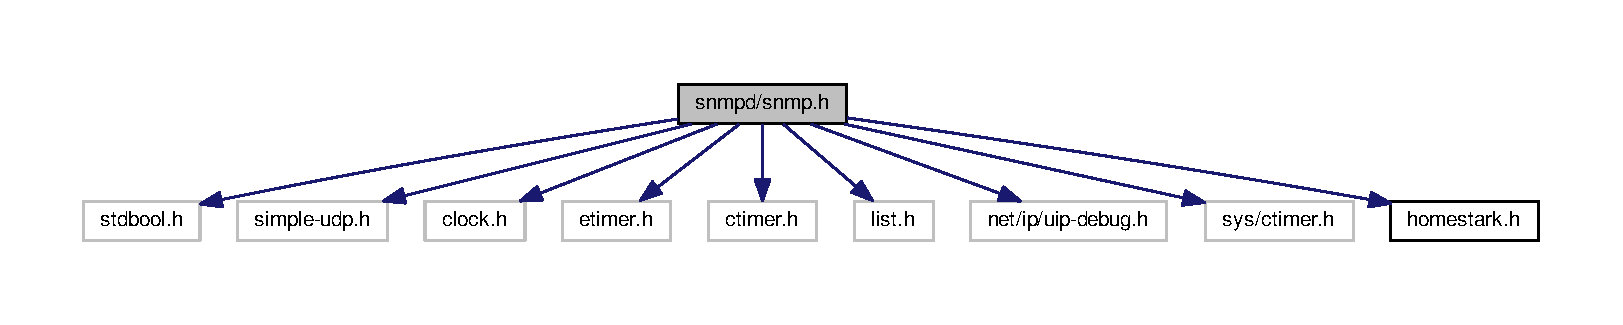
\includegraphics[width=350pt]{snmp_8h__incl}
\end{center}
\end{figure}
Este grafo mostra quais são os ficheiros que incluem directamente ou indirectamente este ficheiro\+:\nopagebreak
\begin{figure}[H]
\begin{center}
\leavevmode
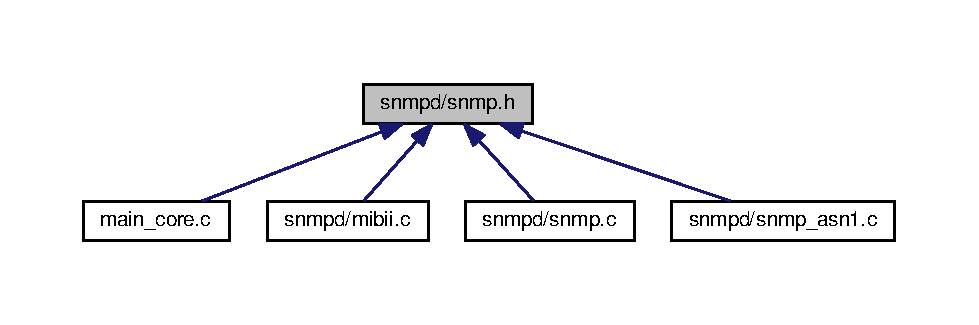
\includegraphics[width=350pt]{snmp_8h__dep__incl}
\end{center}
\end{figure}
\subsection*{Estruturas de Dados}
\begin{DoxyCompactItemize}
\item 
struct \hyperlink{structsnmp__t}{snmp\+\_\+t}
\begin{DoxyCompactList}\small\item\em Struct for the S\+N\+M\+P Message. \end{DoxyCompactList}\item 
struct \hyperlink{structrequest}{request}
\begin{DoxyCompactList}\small\item\em Struct for request of S\+N\+M\+P Packets. \end{DoxyCompactList}\end{DoxyCompactItemize}
\subsection*{Macros}
\begin{DoxyCompactItemize}
\item 
\hypertarget{snmp_8h_abb9d473894655ab94b1dca8f0ef5fa1d}{\#define \hyperlink{snmp_8h_abb9d473894655ab94b1dca8f0ef5fa1d}{D\+E\+F\+A\+U\+L\+T\+\_\+\+S\+N\+M\+P\+\_\+\+P\+O\+R\+T}~161}\label{snmp_8h_abb9d473894655ab94b1dca8f0ef5fa1d}

\begin{DoxyCompactList}\small\item\em Default S\+N\+M\+P Agent port. \end{DoxyCompactList}\item 
\hypertarget{snmp_8h_abe670cc5ceed3fad3be682fc0c1bb62e}{\#define \hyperlink{snmp_8h_abe670cc5ceed3fad3be682fc0c1bb62e}{E\+R\+R\+O\+R\+\_\+\+N\+O\+N\+E}~0x00 /$\ast$$\ast$  @brief No error occurred $\ast$/}\label{snmp_8h_abe670cc5ceed3fad3be682fc0c1bb62e}

\begin{DoxyCompactList}\small\item\em Types of errors in S\+N\+M\+P P\+D\+U. \end{DoxyCompactList}\item 
\hypertarget{snmp_8h_af32d4348918915bc367cc37feee380aa}{\#define {\bfseries E\+R\+R\+O\+R\+\_\+\+R\+E\+S\+P\+\_\+\+T\+O\+O\+\_\+\+L\+A\+R\+G\+E}~0x01 /$\ast$$\ast$  @brief Response message too large to transpor $\ast$/}\label{snmp_8h_af32d4348918915bc367cc37feee380aa}

\item 
\hypertarget{snmp_8h_a9c68a3cb2a8ed6cc0ecc1b90e153a4d6}{\#define {\bfseries E\+R\+R\+O\+R\+\_\+\+R\+E\+Q\+\_\+\+O\+I\+D\+\_\+\+N\+O\+T\+\_\+\+F\+O\+U\+N\+D}~0x02 /$\ast$$\ast$  @brief The name of the requested object was not found $\ast$/}\label{snmp_8h_a9c68a3cb2a8ed6cc0ecc1b90e153a4d6}

\item 
\hypertarget{snmp_8h_aa645c4ae323d9c46969ad9e8c1cc759f}{\#define {\bfseries E\+R\+R\+O\+R\+\_\+\+D\+A\+T\+A\+\_\+\+T\+Y\+P\+E\+\_\+\+M\+A\+T\+C\+H}~0x03 /$\ast$$\ast$  @brief A data type in the request did not match the data type in the S\+N\+M\+P agent $\ast$/}\label{snmp_8h_aa645c4ae323d9c46969ad9e8c1cc759f}

\item 
\hypertarget{snmp_8h_aa9f64367e63ebe993445b600e21a9d7c}{\#define {\bfseries E\+R\+R\+O\+R\+\_\+\+M\+A\+N\+\_\+\+R\+E\+A\+D\+\_\+\+O\+N\+L\+Y}~0x04 /$\ast$$\ast$  @brief The S\+N\+M\+P manager attempted to set a read-\/only parameter $\ast$/}\label{snmp_8h_aa9f64367e63ebe993445b600e21a9d7c}

\item 
\hypertarget{snmp_8h_a157030e577ab0802e022ff053c8e2425}{\#define {\bfseries E\+R\+R\+O\+R\+\_\+\+G\+E\+N\+E\+R\+A\+L}~0x05 /$\ast$$\ast$  @brief General Error (some error other than the ones listed above) $\ast$/}\label{snmp_8h_a157030e577ab0802e022ff053c8e2425}

\item 
\hypertarget{snmp_8h_a45fec4a033960bca8c60e2f40d1d0e04}{\#define \hyperlink{snmp_8h_a45fec4a033960bca8c60e2f40d1d0e04}{A\+S\+N1\+\_\+\+P\+R\+I\+M\+\_\+\+I\+N\+T\+E\+G\+E\+R}~0x02}\label{snmp_8h_a45fec4a033960bca8c60e2f40d1d0e04}

\begin{DoxyCompactList}\small\item\em Primitives data types of A\+N\+S.\+1 encoding. \end{DoxyCompactList}\item 
\hypertarget{snmp_8h_a527d19e9c9039d5be00f7a16072f848d}{\#define {\bfseries A\+S\+N1\+\_\+\+P\+R\+I\+M\+\_\+\+O\+C\+T\+\_\+\+S\+T\+R}~0x04}\label{snmp_8h_a527d19e9c9039d5be00f7a16072f848d}

\item 
\hypertarget{snmp_8h_a9ba0818a12a0200e430936492f575207}{\#define {\bfseries A\+S\+N1\+\_\+\+P\+R\+I\+M\+\_\+\+N\+U\+L\+L}~0x05}\label{snmp_8h_a9ba0818a12a0200e430936492f575207}

\item 
\hypertarget{snmp_8h_a4168ea3604dfb4452b63f916baa77db6}{\#define {\bfseries A\+S\+N1\+\_\+\+P\+R\+I\+M\+\_\+\+O\+I\+D}~0x06}\label{snmp_8h_a4168ea3604dfb4452b63f916baa77db6}

\item 
\hypertarget{snmp_8h_a23bdc4d15d908a80e4bc06be55463ffc}{\#define \hyperlink{snmp_8h_a23bdc4d15d908a80e4bc06be55463ffc}{M\+A\+X\+\_\+\+O\+C\+T\+E\+T\+\_\+\+S\+T\+R\+I\+N\+G}~0x\+F\+A}\label{snmp_8h_a23bdc4d15d908a80e4bc06be55463ffc}

\begin{DoxyCompactList}\small\item\em Max data types in each kind of variable. \end{DoxyCompactList}\item 
\hypertarget{snmp_8h_a4cb667ecd24e47e91d466b83f149ac1a}{\#define {\bfseries M\+A\+X\+\_\+\+O\+I\+D\+\_\+\+S\+T\+R\+I\+N\+G}~20}\label{snmp_8h_a4cb667ecd24e47e91d466b83f149ac1a}

\item 
\hypertarget{snmp_8h_a0317937adfd3502cbe39a0ea9e6e5b51}{\#define {\bfseries M\+A\+X\+\_\+\+U\+D\+P\+\_\+\+S\+N\+M\+P}~300}\label{snmp_8h_a0317937adfd3502cbe39a0ea9e6e5b51}

\item 
\hypertarget{snmp_8h_aa4d923102cb2314e31cbf833482e9090}{\#define \hyperlink{snmp_8h_aa4d923102cb2314e31cbf833482e9090}{A\+S\+N1\+\_\+\+C\+P\+X\+\_\+\+S\+E\+Q\+U\+E\+N\+C\+E}~0x30}\label{snmp_8h_aa4d923102cb2314e31cbf833482e9090}

\begin{DoxyCompactList}\small\item\em Complex data types of A\+N\+S.\+1 encoding. \end{DoxyCompactList}\item 
\hypertarget{snmp_8h_a60e229998bcd49b627bd7de12b4213fc}{\#define {\bfseries A\+S\+N1\+\_\+\+C\+P\+X\+\_\+\+G\+E\+T\+\_\+\+R\+E\+Q}~0x\+A0}\label{snmp_8h_a60e229998bcd49b627bd7de12b4213fc}

\item 
\hypertarget{snmp_8h_a19fce71c9def4f2eb9c1a56025cdd6e6}{\#define {\bfseries A\+S\+N1\+\_\+\+C\+P\+X\+\_\+\+N\+E\+X\+T\+\_\+\+R\+E\+Q}~0x\+A1}\label{snmp_8h_a19fce71c9def4f2eb9c1a56025cdd6e6}

\item 
\hypertarget{snmp_8h_a04bfde48c8f821965706cdbf272c07da}{\#define {\bfseries A\+S\+N1\+\_\+\+C\+P\+X\+\_\+\+G\+E\+T\+\_\+\+R\+E\+S\+P}~0x\+A2}\label{snmp_8h_a04bfde48c8f821965706cdbf272c07da}

\item 
\hypertarget{snmp_8h_a0de2cd3eb4c4bd22e91b3b69c86069bc}{\#define {\bfseries A\+S\+N1\+\_\+\+C\+P\+X\+\_\+\+S\+E\+T\+\_\+\+R\+E\+Q}~0x\+A3}\label{snmp_8h_a0de2cd3eb4c4bd22e91b3b69c86069bc}

\item 
\hypertarget{snmp_8h_ab6614668ab182944f672a21c1d3cb581}{\#define {\bfseries M\+A\+X\+\_\+\+O\+I\+D\+S}~14             /$\ast$$\ast$ @brief Number max. of address that the device will answer about M\+I\+B Implementation $\ast$/}\label{snmp_8h_ab6614668ab182944f672a21c1d3cb581}

\item 
\hypertarget{snmp_8h_a62f5a786eeaa68ffaa9daf2856501283}{\#define {\bfseries M\+A\+X\+\_\+\+S\+T\+R\+I\+N\+G\+S\+\_\+\+L\+E\+N\+G\+T\+H}~100            /$\ast$$\ast$ @brief Max length of string in the O\+I\+D Implementation $\ast$/}\label{snmp_8h_a62f5a786eeaa68ffaa9daf2856501283}

\item 
\hypertarget{snmp_8h_a9590682504e9a26892b76a0ceabf6278}{\#define {\bfseries T\+I\+M\+E\+\_\+\+U\+P\+D\+A\+T\+E\+\_\+\+S\+N\+M\+P}~2$\ast$C\+L\+O\+C\+K\+\_\+\+S\+E\+C\+O\+N\+D /$\ast$$\ast$ @brief Time to update the O\+I\+Ds of M\+I\+B implementation $\ast$/}\label{snmp_8h_a9590682504e9a26892b76a0ceabf6278}

\item 
\hypertarget{snmp_8h_a1f1b7fadcf29f1de5bb406bf356c1d71}{\#define \hyperlink{snmp_8h_a1f1b7fadcf29f1de5bb406bf356c1d71}{S\+N\+M\+P\+\_\+\+V\+E\+R\+S\+I\+O\+N\+\_\+1}~0}\label{snmp_8h_a1f1b7fadcf29f1de5bb406bf356c1d71}

\begin{DoxyCompactList}\small\item\em value of the version field for the S\+N\+M\+Pv1 \end{DoxyCompactList}\item 
\hypertarget{snmp_8h_a0599530b4b198b2c7fa49a274f3f3878}{\#define \hyperlink{snmp_8h_a0599530b4b198b2c7fa49a274f3f3878}{S\+N\+M\+P\+\_\+\+V\+E\+R\+S\+I\+O\+N\+\_\+2\+C}~1}\label{snmp_8h_a0599530b4b198b2c7fa49a274f3f3878}

\begin{DoxyCompactList}\small\item\em value of the version field for the S\+N\+M\+Pv2c \end{DoxyCompactList}\item 
\hypertarget{snmp_8h_aa0b283beac3c7da5c28058f52a817c0c}{\#define \hyperlink{snmp_8h_aa0b283beac3c7da5c28058f52a817c0c}{S\+N\+M\+P\+\_\+\+V\+E\+R\+S\+I\+O\+N\+\_\+3}~3}\label{snmp_8h_aa0b283beac3c7da5c28058f52a817c0c}

\begin{DoxyCompactList}\small\item\em value of the version field for the S\+N\+M\+Pv3 \end{DoxyCompactList}\item 
\hypertarget{snmp_8h_a388ebedb8b344492bded4ba233fab27d}{\#define \hyperlink{snmp_8h_a388ebedb8b344492bded4ba233fab27d}{check\+\_\+seq}(x)~(x == \hyperlink{snmp_8h_aa4d923102cb2314e31cbf833482e9090}{A\+S\+N1\+\_\+\+C\+P\+X\+\_\+\+S\+E\+Q\+U\+E\+N\+C\+E} ? 1 \+: 0)}\label{snmp_8h_a388ebedb8b344492bded4ba233fab27d}

\begin{DoxyCompactList}\small\item\em Decode the initial sequence type. \end{DoxyCompactList}\item 
\hypertarget{snmp_8h_a8e7df5e1bbe7073bba31a017a76ae7c3}{\#define {\bfseries D\+E\+B\+U\+G\+\_\+\+S\+N\+M\+P\+\_\+\+D\+E\+C\+O\+D\+I\+N\+G}~/$\ast$$\ast$ @brief If defined, show decode S\+N\+M\+P messages $\ast$/}\label{snmp_8h_a8e7df5e1bbe7073bba31a017a76ae7c3}

\item 
\hypertarget{snmp_8h_a93706e3dc38501c9cb9f4cdfaebb1758}{\#define {\bfseries D\+E\+B\+U\+G\+\_\+\+S\+N\+M\+P}~/$\ast$$\ast$ @brief Enable S\+N\+M\+P Debug message $\ast$/}\label{snmp_8h_a93706e3dc38501c9cb9f4cdfaebb1758}

\item 
\hypertarget{snmp_8h_a53394c5715c5354d04dda91cd6badf9a}{\#define {\bfseries debug\+\_\+snmp}(fmt, args...)~printf(\char`\"{}\textbackslash{}n\mbox{[}S\+N\+M\+P\mbox{]} \char`\"{}fmt, \#\#args)}\label{snmp_8h_a53394c5715c5354d04dda91cd6badf9a}

\end{DoxyCompactItemize}
\subsection*{Enumerações}
\begin{DoxyCompactItemize}
\item 
enum \hyperlink{snmp_8h_add91ba4199db8665b9b9fc56fc6783a6}{resp\+\_\+con\+\_\+t} \{ \hyperlink{snmp_8h_add91ba4199db8665b9b9fc56fc6783a6ac6ae922662cbaf7958eb387bfd6fe4da}{F\+A\+I\+L\+\_\+\+C\+O\+N}, 
\hyperlink{snmp_8h_add91ba4199db8665b9b9fc56fc6783a6ae7b7a388c90c2c5428cced225760885f}{S\+U\+C\+C\+E\+S\+S\+\_\+\+C\+O\+N}
 \}
\begin{DoxyCompactList}\small\item\em Type of errors in S\+N\+M\+P functions. \end{DoxyCompactList}\end{DoxyCompactItemize}
\subsection*{Funções}
\begin{DoxyCompactItemize}
\item 
\hyperlink{snmp_8h_add91ba4199db8665b9b9fc56fc6783a6}{resp\+\_\+con\+\_\+t} \hyperlink{snmp_8h_a0c7f91118bbe8cf32398c753ead2b7f2}{decode\+\_\+asn1\+\_\+oct\+\_\+str} (uint8\+\_\+t $\ast$data\+\_\+encoded, uint8\+\_\+t $\ast$oct\+\_\+str)
\begin{DoxyCompactList}\small\item\em S\+N\+M\+P Decode Octet String. \end{DoxyCompactList}\item 
\hyperlink{snmp_8h_add91ba4199db8665b9b9fc56fc6783a6}{resp\+\_\+con\+\_\+t} \hyperlink{snmp_8h_acb3a9652e9b960748692caef7f443384}{decode\+\_\+asn1\+\_\+integer} (uint8\+\_\+t $\ast$data\+\_\+encoded, uint32\+\_\+t $\ast$integer\+\_\+value)
\begin{DoxyCompactList}\small\item\em S\+N\+M\+P Decode Integer. \end{DoxyCompactList}\item 
\hyperlink{snmp_8h_add91ba4199db8665b9b9fc56fc6783a6}{resp\+\_\+con\+\_\+t} \hyperlink{snmp_8h_aca484712bcdb0bbc0f065061c4a0ed20}{snmp\+\_\+decode\+\_\+message} (char $\ast$snmp\+\_\+packet, \hyperlink{structsnmp__t}{snmp\+\_\+t} $\ast$v)
\begin{DoxyCompactList}\small\item\em Decode S\+N\+M\+P message. \end{DoxyCompactList}\item 
uint16\+\_\+t \hyperlink{snmp_8h_a63d8ffecf9aa0af9824de046643c140f}{snmp\+\_\+encode\+\_\+message} (\hyperlink{structsnmp__t}{snmp\+\_\+t} $\ast$snmp\+\_\+handle, char $\ast$data\+\_\+encoded)
\begin{DoxyCompactList}\small\item\em Encode S\+N\+M\+P message. \end{DoxyCompactList}\item 
int \hyperlink{snmp_8h_a523ab718dec1a794b3f8c8752f1e2ae3}{ipaddr\+\_\+sprintf} (char $\ast$buf, uint8\+\_\+t buf\+\_\+len, const uip\+\_\+ipaddr\+\_\+t $\ast$addr)
\begin{DoxyCompactList}\small\item\em Convert I\+Pv6 address in char format. \end{DoxyCompactList}\item 
void \hyperlink{snmp_8h_a05848f4eb62dd417b99e461854870bf9}{snmp\+\_\+cb\+\_\+data} (void)
\begin{DoxyCompactList}\small\item\em S\+N\+M\+P Callback receive. \end{DoxyCompactList}\item 
void \hyperlink{snmp_8h_a4d88f2fc7655280384131d543e0d83e5}{snmp\+\_\+init} (void)
\begin{DoxyCompactList}\small\item\em S\+N\+M\+P Init function. \end{DoxyCompactList}\item 
void \hyperlink{snmp_8h_a732192a9e72d3182d395c47e2cd9c79e}{update\+\_\+snmp\+\_\+mib} (void)
\begin{DoxyCompactList}\small\item\em Update S\+N\+M\+P O\+I\+Ds. \end{DoxyCompactList}\end{DoxyCompactItemize}
\subsection*{Variáveis}
\begin{DoxyCompactItemize}
\item 
\hypertarget{snmp_8h_ab81bbe09328677d32f662e865f20b0bd}{struct \hyperlink{structrequest}{request} $\ast$ {\bfseries request\+\_\+first}}\label{snmp_8h_ab81bbe09328677d32f662e865f20b0bd}

\item 
\hypertarget{snmp_8h_a3e7b17f11bc27215e1f0e52de3d1a92e}{struct \hyperlink{structrequest}{request} $\ast$ {\bfseries request\+\_\+last}}\label{snmp_8h_a3e7b17f11bc27215e1f0e52de3d1a92e}

\end{DoxyCompactItemize}


\subsection{Descrição detalhada}
Licensed to the Apache Software Foundation (A\+S\+F) under one or more contributor license agreements. 

See the N\+O\+T\+I\+C\+E file distributed with this work for additional information regarding copyright ownership. The A\+S\+F licenses this file to you under the Apache License, Version 2.\+0 (the \char`\"{}\+License\char`\"{}); you may not use this file except in compliance with the License. You may obtain a copy of the License at

\href{http://www.apache.org/licenses/LICENSE-2.0}{\tt http\+://www.\+apache.\+org/licenses/\+L\+I\+C\+E\+N\+S\+E-\/2.\+0}

Unless required by applicable law or agreed to in writing, software distributed under the License is distributed on an \char`\"{}\+A\+S I\+S\char`\"{} B\+A\+S\+I\+S, W\+I\+T\+H\+O\+U\+T W\+A\+R\+R\+A\+N\+T\+I\+E\+S O\+R C\+O\+N\+D\+I\+T\+I\+O\+N\+S O\+F A\+N\+Y K\+I\+N\+D, either express or implied. See the License for the specific language governing permissions and limitations under the License.

This project is delivered under Apache 2.\+0 license.

Header functions about S\+N\+M\+P implementation \begin{DoxyAuthor}{Autor}
Ânderson Ignácio da Silva 
\end{DoxyAuthor}
\begin{DoxyDate}{Data}
12 Sept 2016 
\end{DoxyDate}
\begin{DoxySeeAlso}{Veja também}
\href{http://www.aignacio.com}{\tt http\+://www.\+aignacio.\+com} 
\end{DoxySeeAlso}


\subsection{Documentação dos valores da enumeração}
\hypertarget{snmp_8h_add91ba4199db8665b9b9fc56fc6783a6}{\index{snmp.\+h@{snmp.\+h}!resp\+\_\+con\+\_\+t@{resp\+\_\+con\+\_\+t}}
\index{resp\+\_\+con\+\_\+t@{resp\+\_\+con\+\_\+t}!snmp.\+h@{snmp.\+h}}
\subsubsection[{resp\+\_\+con\+\_\+t}]{\setlength{\rightskip}{0pt plus 5cm}enum {\bf resp\+\_\+con\+\_\+t}}}\label{snmp_8h_add91ba4199db8665b9b9fc56fc6783a6}


Type of errors in S\+N\+M\+P functions. 

\begin{Desc}
\item[Valores da enumeração]\par
\begin{description}
\index{F\+A\+I\+L\+\_\+\+C\+O\+N@{F\+A\+I\+L\+\_\+\+C\+O\+N}!snmp.\+h@{snmp.\+h}}\index{snmp.\+h@{snmp.\+h}!F\+A\+I\+L\+\_\+\+C\+O\+N@{F\+A\+I\+L\+\_\+\+C\+O\+N}}\item[{\em 
\hypertarget{snmp_8h_add91ba4199db8665b9b9fc56fc6783a6ac6ae922662cbaf7958eb387bfd6fe4da}{F\+A\+I\+L\+\_\+\+C\+O\+N}\label{snmp_8h_add91ba4199db8665b9b9fc56fc6783a6ac6ae922662cbaf7958eb387bfd6fe4da}
}]Error to to process function. \index{S\+U\+C\+C\+E\+S\+S\+\_\+\+C\+O\+N@{S\+U\+C\+C\+E\+S\+S\+\_\+\+C\+O\+N}!snmp.\+h@{snmp.\+h}}\index{snmp.\+h@{snmp.\+h}!S\+U\+C\+C\+E\+S\+S\+\_\+\+C\+O\+N@{S\+U\+C\+C\+E\+S\+S\+\_\+\+C\+O\+N}}\item[{\em 
\hypertarget{snmp_8h_add91ba4199db8665b9b9fc56fc6783a6ae7b7a388c90c2c5428cced225760885f}{S\+U\+C\+C\+E\+S\+S\+\_\+\+C\+O\+N}\label{snmp_8h_add91ba4199db8665b9b9fc56fc6783a6ae7b7a388c90c2c5428cced225760885f}
}]Sucess to process function. \begin{DoxyRefDesc}{Tarefa}
\item[\hyperlink{todo__todo000001}{Tarefa}]Implement more kind of errors \end{DoxyRefDesc}
\end{description}
\end{Desc}

\begin{DoxyCode}
129              \{
130    \hyperlink{snmp_8h_add91ba4199db8665b9b9fc56fc6783a6ac6ae922662cbaf7958eb387bfd6fe4da}{FAIL\_CON},
131    \hyperlink{snmp_8h_add91ba4199db8665b9b9fc56fc6783a6ae7b7a388c90c2c5428cced225760885f}{SUCCESS\_CON},
132 \} \hyperlink{snmp_8h_add91ba4199db8665b9b9fc56fc6783a6}{resp\_con\_t};
\end{DoxyCode}


\subsection{Documentação das funções}
\hypertarget{snmp_8h_acb3a9652e9b960748692caef7f443384}{\index{snmp.\+h@{snmp.\+h}!decode\+\_\+asn1\+\_\+integer@{decode\+\_\+asn1\+\_\+integer}}
\index{decode\+\_\+asn1\+\_\+integer@{decode\+\_\+asn1\+\_\+integer}!snmp.\+h@{snmp.\+h}}
\subsubsection[{decode\+\_\+asn1\+\_\+integer}]{\setlength{\rightskip}{0pt plus 5cm}{\bf resp\+\_\+con\+\_\+t} decode\+\_\+asn1\+\_\+integer (
\begin{DoxyParamCaption}
\item[{uint8\+\_\+t $\ast$}]{data\+\_\+encoded, }
\item[{uint32\+\_\+t $\ast$}]{integer\+\_\+value}
\end{DoxyParamCaption}
)}}\label{snmp_8h_acb3a9652e9b960748692caef7f443384}


S\+N\+M\+P Decode Integer. 

Decode A\+S\+N.\+1 integer(32 bit value).


\begin{DoxyParams}[1]{Parâmetros}
\mbox{\tt in}  & {\em data\+\_\+encoded} & Data do decode \\
\hline
\mbox{\tt in}  & {\em integer\+\_\+value} & Variable the will receive the integer 32-\/bit\\
\hline
\end{DoxyParams}

\begin{DoxyRetVals}{Valores retornados}
{\em S\+U\+C\+C\+E\+S\+S\+\_\+\+C\+O\+N} & Success to decode integer \\
\hline
{\em F\+A\+I\+L\+\_\+\+C\+O\+N} & Fail to decode integer \\
\hline
\end{DoxyRetVals}

\begin{DoxyCode}
91                                                                               \{
92   uint8\_t length = (intptr\_t)*(data\_encoded+1);
93   \textcolor{comment}{// uint32\_t integer\_value;}
94   \textcolor{keywordtype}{size\_t} i = 0;
95   uint32\_t aux;
96 
97   \textcolor{comment}{// Test if it's an integer value to be decoded}
98   \textcolor{keywordflow}{if} (*data\_encoded != \hyperlink{snmp_8h_a45fec4a033960bca8c60e2f40d1d0e04}{ASN1\_PRIM\_INTEGER})\{
99     debug\_snmp(\textcolor{stringliteral}{"The value is not integer!"});
100     \textcolor{keywordflow}{return} \hyperlink{snmp_8h_add91ba4199db8665b9b9fc56fc6783a6ac6ae922662cbaf7958eb387bfd6fe4da}{FAIL\_CON};
101   \}
102 
103   \textcolor{keywordflow}{for} (i=1, *integer\_value = 0; i <= length; i++)\{
104     aux = *(data\_encoded+1+i);
105     *integer\_value += aux*(pow(256,(length-i)));
106     \textcolor{comment}{// debug\_snmp("%lu * 256^%d = %lu",aux,(length-i),*integer\_value);}
107   \}
108   \textcolor{keywordflow}{return} \hyperlink{snmp_8h_add91ba4199db8665b9b9fc56fc6783a6ae7b7a388c90c2c5428cced225760885f}{SUCCESS\_CON};
109 \}
\end{DoxyCode}
\hypertarget{snmp_8h_a0c7f91118bbe8cf32398c753ead2b7f2}{\index{snmp.\+h@{snmp.\+h}!decode\+\_\+asn1\+\_\+oct\+\_\+str@{decode\+\_\+asn1\+\_\+oct\+\_\+str}}
\index{decode\+\_\+asn1\+\_\+oct\+\_\+str@{decode\+\_\+asn1\+\_\+oct\+\_\+str}!snmp.\+h@{snmp.\+h}}
\subsubsection[{decode\+\_\+asn1\+\_\+oct\+\_\+str}]{\setlength{\rightskip}{0pt plus 5cm}{\bf resp\+\_\+con\+\_\+t} decode\+\_\+asn1\+\_\+oct\+\_\+str (
\begin{DoxyParamCaption}
\item[{uint8\+\_\+t $\ast$}]{data\+\_\+encoded, }
\item[{uint8\+\_\+t $\ast$}]{oct\+\_\+str}
\end{DoxyParamCaption}
)}}\label{snmp_8h_a0c7f91118bbe8cf32398c753ead2b7f2}


S\+N\+M\+P Decode Octet String. 

Decode Octet String in A\+S\+N.\+1 format.


\begin{DoxyParams}[1]{Parâmetros}
\mbox{\tt in}  & {\em data\+\_\+encoded} & Data do decode \\
\hline
\mbox{\tt in}  & {\em oct\+\_\+str} & Variable the will receive the octet string\\
\hline
\end{DoxyParams}

\begin{DoxyRetVals}{Valores retornados}
{\em S\+U\+C\+C\+E\+S\+S\+\_\+\+C\+O\+N} & Success to decode string octet \\
\hline
{\em F\+A\+I\+L\+\_\+\+C\+O\+N} & Fail to decode octet string \\
\hline
\end{DoxyRetVals}

\begin{DoxyCode}
72                                                                        \{
73   \textcolor{keywordflow}{if} (*data\_encoded !=  (intptr\_t)ASN1\_PRIM\_OCT\_STR) \{
74     debug\_snmp(\textcolor{stringliteral}{"The type of value passed is not an octet string!"});
75     \textcolor{keywordflow}{return} \hyperlink{snmp_8h_add91ba4199db8665b9b9fc56fc6783a6ac6ae922662cbaf7958eb387bfd6fe4da}{FAIL\_CON};
76   \}
77 
78   uint8\_t length = (intptr\_t)*(data\_encoded+1),
79           index = 0;
80   \textcolor{keywordflow}{while} (length) \{
81     *(oct\_str+index) = (intptr\_t)*(data\_encoded+2+index);
82     length--;
83     index++;
84   \}
85 
86   *(oct\_str+index) = \textcolor{charliteral}{'\(\backslash\)0'};
87   \textcolor{comment}{// printf("\(\backslash\)nEndereco----:> %d\(\backslash\)n",oct\_str);}
88   \textcolor{keywordflow}{return} \hyperlink{snmp_8h_add91ba4199db8665b9b9fc56fc6783a6ae7b7a388c90c2c5428cced225760885f}{SUCCESS\_CON};
89 \}
\end{DoxyCode}
\hypertarget{snmp_8h_a523ab718dec1a794b3f8c8752f1e2ae3}{\index{snmp.\+h@{snmp.\+h}!ipaddr\+\_\+sprintf@{ipaddr\+\_\+sprintf}}
\index{ipaddr\+\_\+sprintf@{ipaddr\+\_\+sprintf}!snmp.\+h@{snmp.\+h}}
\subsubsection[{ipaddr\+\_\+sprintf}]{\setlength{\rightskip}{0pt plus 5cm}int ipaddr\+\_\+sprintf (
\begin{DoxyParamCaption}
\item[{char $\ast$}]{buf, }
\item[{uint8\+\_\+t}]{buf\+\_\+len, }
\item[{const uip\+\_\+ipaddr\+\_\+t $\ast$}]{addr}
\end{DoxyParamCaption}
)}}\label{snmp_8h_a523ab718dec1a794b3f8c8752f1e2ae3}


Convert I\+Pv6 address in char format. 

Format I\+Pv6 address in string char variable.


\begin{DoxyParams}[1]{Parâmetros}
\mbox{\tt in}  & {\em buf} & Variable that'll receive the ipv6 address decoded \\
\hline
\mbox{\tt in}  & {\em buf\+\_\+len} & Len of buf variable \\
\hline
\mbox{\tt in}  & {\em addr} & Address I\+Pv6 in uip\+\_\+ipaddr\+\_\+t format\\
\hline
\end{DoxyParams}

\begin{DoxyRetVals}{Valores retornados}
{\em len} & Length of buf variable formated \\
\hline
\end{DoxyRetVals}

\begin{DoxyCode}
101                                                                          \{
102   uint16\_t a;
103   uint8\_t len = 0;
104   \textcolor{keywordtype}{int} i, f;
105   \textcolor{keywordflow}{for}(i = 0, f = 0; i < \textcolor{keyword}{sizeof}(uip\_ipaddr\_t); i += 2) \{
106     a = (addr->u8[i] << 8) + addr->u8[i + 1];
107     \textcolor{keywordflow}{if}(a == 0 && f >= 0) \{
108       \textcolor{keywordflow}{if}(f++ == 0) \{
109         len += snprintf(&buf[len], buf\_len - len, \textcolor{stringliteral}{"::"});
110       \}
111     \} \textcolor{keywordflow}{else} \{
112       \textcolor{keywordflow}{if}(f > 0) \{
113         f = -1;
114       \} \textcolor{keywordflow}{else} \textcolor{keywordflow}{if}(i > 0) \{
115         len += snprintf(&buf[len], buf\_len - len, \textcolor{stringliteral}{":"});
116       \}
117       len += snprintf(&buf[len], buf\_len - len, \textcolor{stringliteral}{"%x"}, a);
118     \}
119   \}
120 
121   \textcolor{keywordflow}{return} len;
122 \}
\end{DoxyCode}
\hypertarget{snmp_8h_a05848f4eb62dd417b99e461854870bf9}{\index{snmp.\+h@{snmp.\+h}!snmp\+\_\+cb\+\_\+data@{snmp\+\_\+cb\+\_\+data}}
\index{snmp\+\_\+cb\+\_\+data@{snmp\+\_\+cb\+\_\+data}!snmp.\+h@{snmp.\+h}}
\subsubsection[{snmp\+\_\+cb\+\_\+data}]{\setlength{\rightskip}{0pt plus 5cm}void snmp\+\_\+cb\+\_\+data (
\begin{DoxyParamCaption}
\item[{void}]{}
\end{DoxyParamCaption}
)}}\label{snmp_8h_a05848f4eb62dd417b99e461854870bf9}


S\+N\+M\+P Callback receive. 

Receive in callback mode, any data from N\+M\+S of S\+N\+M\+P protocol.


\begin{DoxyParams}[1]{Parâmetros}
\mbox{\tt in}  & {\em void} & No argument to pass\\
\hline
\end{DoxyParams}

\begin{DoxyRetVals}{Valores retornados}
{\em void} & Doesn't return anything \\
\hline
\end{DoxyRetVals}

\begin{DoxyCode}
71                        \{
72   \textcolor{keyword}{static} uint16\_t len;
73   \textcolor{keyword}{static} \textcolor{keywordtype}{char} buf[MAX\_UDP\_SNMP];
74   memset(buf, 0, MAX\_UDP\_SNMP);
75 
76   \textcolor{keywordflow}{if}(uip\_newdata()) \{
77     len = uip\_datalen();
78     memcpy(buf, uip\_appdata, len);
79     debug\_snmp(\textcolor{stringliteral}{"%u bytes from ["}, len);
80     uip\_debug\_ipaddr\_print(&UIP\_IP\_BUF->srcipaddr);
81     printf(\textcolor{stringliteral}{"]:%u"}, UIP\_HTONS(UIP\_UDP\_BUF->srcport));
82     uip\_ipaddr\_copy(&server\_conn->ripaddr, &UIP\_IP\_BUF->srcipaddr);
83     server\_conn->rport = UIP\_UDP\_BUF->srcport;
84     \hyperlink{structsnmp__t}{snmp\_t} snmp\_handle;
85     \textcolor{keywordflow}{if} (\hyperlink{snmp_8h_aca484712bcdb0bbc0f065061c4a0ed20}{snmp\_decode\_message}(buf, &snmp\_handle))\{
86       debug\_snmp(\textcolor{stringliteral}{"New SNMP Request received!"});
87       len = \hyperlink{snmp_8h_a63d8ffecf9aa0af9824de046643c140f}{snmp\_encode\_message}(&snmp\_handle, buf);
88       uip\_udp\_packet\_send(server\_conn, buf, len);
89       uip\_create\_unspecified(&server\_conn->ripaddr);
90       server\_conn->rport = 0;
91     \}
92     \textcolor{keywordflow}{else}
93       debug\_snmp(\textcolor{stringliteral}{"Problem on SNMP Request received!"});
94   \}
95 \}
\end{DoxyCode}
\hypertarget{snmp_8h_aca484712bcdb0bbc0f065061c4a0ed20}{\index{snmp.\+h@{snmp.\+h}!snmp\+\_\+decode\+\_\+message@{snmp\+\_\+decode\+\_\+message}}
\index{snmp\+\_\+decode\+\_\+message@{snmp\+\_\+decode\+\_\+message}!snmp.\+h@{snmp.\+h}}
\subsubsection[{snmp\+\_\+decode\+\_\+message}]{\setlength{\rightskip}{0pt plus 5cm}{\bf resp\+\_\+con\+\_\+t} snmp\+\_\+decode\+\_\+message (
\begin{DoxyParamCaption}
\item[{char $\ast$}]{snmp\+\_\+packet, }
\item[{{\bf snmp\+\_\+t} $\ast$}]{v}
\end{DoxyParamCaption}
)}}\label{snmp_8h_aca484712bcdb0bbc0f065061c4a0ed20}


Decode S\+N\+M\+P message. 

Decode a S\+N\+M\+P message v1 and format to answer request.


\begin{DoxyParams}[1]{Parâmetros}
\mbox{\tt in}  & {\em snmp\+\_\+packet} & Data U\+D\+P -\/ S\+N\+M\+P to decode \\
\hline
\mbox{\tt in}  & {\em snmp\+\_\+handle} & Struct that will receive the S\+N\+M\+P request messsage\\
\hline
\end{DoxyParams}

\begin{DoxyRetVals}{Valores retornados}
{\em S\+U\+C\+C\+E\+S\+S\+\_\+\+C\+O\+N} & Success to decode S\+N\+M\+P Message \\
\hline
{\em F\+A\+I\+L\+\_\+\+C\+O\+N} & Fail to decode S\+N\+M\+P Message \\
\hline
\end{DoxyRetVals}

\begin{DoxyCode}
111                                                                       \{
112   uint8\_t buffer[50], aux;
113   \textcolor{keywordtype}{size\_t} i;
114 
115 \textcolor{preprocessor}{  #ifdef DEBUG\_SNMP\_DECODING}
116   \textcolor{comment}{// debug\_snmp("Encoded SNMP packet:\(\backslash\)n\(\backslash\)t");}
117   \textcolor{comment}{// for (i=0, j=0; i < *(snmp\_packet+1)+1; j++, i++)\{}
118   \textcolor{comment}{//   if (j > 7)\{}
119   \textcolor{comment}{//     j = 0;}
120   \textcolor{comment}{//     printf("\(\backslash\)n\(\backslash\)t");}
121   \textcolor{comment}{//   \}}
122   \textcolor{comment}{//   printf("[%02x] ",*(snmp\_packet+i));}
123   \textcolor{comment}{// \}}
124 \textcolor{preprocessor}{  #endif}
125 
126   \textcolor{keywordflow}{if} (!\hyperlink{snmp_8h_a388ebedb8b344492bded4ba233fab27d}{check\_seq}(*snmp\_packet))\{
127     debug\_snmp(\textcolor{stringliteral}{"Sequence initial of SNMP message error:%x"},*snmp\_packet);
128     \textcolor{keywordflow}{return} \hyperlink{snmp_8h_add91ba4199db8665b9b9fc56fc6783a6ac6ae922662cbaf7958eb387bfd6fe4da}{FAIL\_CON};
129   \}
130 
131   \textcolor{comment}{/************************ Check the SNMP version ****************************/}
132   \textcolor{keywordflow}{for} (i=0;i < *(snmp\_packet+3)+2; i++)
133     buffer[i] = *(snmp\_packet+2+i);
134   uint32\_t SNMPv = 0;
135   \textcolor{keywordflow}{if} (!\hyperlink{snmp__asn1_8c_acb3a9652e9b960748692caef7f443384}{decode\_asn1\_integer}(buffer,&SNMPv)) \textcolor{keywordflow}{return} \hyperlink{snmp_8h_add91ba4199db8665b9b9fc56fc6783a6ac6ae922662cbaf7958eb387bfd6fe4da}{FAIL\_CON};
136 \textcolor{preprocessor}{  #ifdef DEBUG\_SNMP\_DECODING}
137   debug\_snmp(\textcolor{stringliteral}{"Version SNMP:[1] OK"});
138 \textcolor{preprocessor}{  #endif}
139   \textcolor{keywordflow}{if} (SNMPv != \hyperlink{snmp_8h_a1f1b7fadcf29f1de5bb406bf356c1d71}{SNMP\_VERSION\_1}) \{
140     debug\_snmp(\textcolor{stringliteral}{"SNMP version is different from v1:%lu"},SNMPv);
141     \textcolor{keywordflow}{return} \hyperlink{snmp_8h_add91ba4199db8665b9b9fc56fc6783a6ac6ae922662cbaf7958eb387bfd6fe4da}{FAIL\_CON};
142   \}
143   snmp\_handle->snmp\_version = SNMPv;
144 
145   \textcolor{comment}{/********************** Get the community string ****************************/}
146   \textcolor{keywordflow}{for} (i=0;i < *(snmp\_packet+6)+2; i++)
147   snmp\_handle->community[i] = *(snmp\_packet+5+i);
148   snmp\_handle->community[i] = \textcolor{charliteral}{'\(\backslash\)0'};
149   aux = i;
150 \textcolor{preprocessor}{  #ifdef DEBUG\_SNMP\_DECODING}
151   debug\_snmp(\textcolor{stringliteral}{"Community String: "});
152   \textcolor{keywordflow}{for} (i=0; i < aux; i++)\{
153     \textcolor{keywordflow}{if} (i<2)
154       printf(\textcolor{stringliteral}{"[%d]"},snmp\_handle->community[i]);
155     \textcolor{keywordflow}{else}
156       printf(\textcolor{stringliteral}{"[%c]"},snmp\_handle->community[i]);
157   \}
158 \textcolor{preprocessor}{  #endif}
159 
160   \textcolor{comment}{/************************** Get the request ID ******************************/}
161   aux = 5+snmp\_handle->community[1]+2+2;
162   \textcolor{keywordflow}{for} (i=0;i < *(snmp\_packet+aux+1)+2; i++)
163     snmp\_handle->request\_id\_c[i] = *(snmp\_packet+aux+i);
164   snmp\_handle->request\_id\_c[i] = \textcolor{charliteral}{'\(\backslash\)0'};
165   aux = i;
166 \textcolor{preprocessor}{  #ifdef DEBUG\_SNMP\_DECODING}
167   debug\_snmp(\textcolor{stringliteral}{"Request ID: "});
168   \textcolor{keywordflow}{for} (i=0; i < aux; i++)\{
169     \textcolor{keywordflow}{if} (i<2)
170       printf(\textcolor{stringliteral}{"[%d]"},snmp\_handle->request\_id\_c[i]);
171     \textcolor{keywordflow}{else}
172     printf(\textcolor{stringliteral}{"[%x]"},snmp\_handle->request\_id\_c[i]);
173   \}
174 \textcolor{preprocessor}{  #endif}
175 
176   \textcolor{comment}{/************************** Check for errors ********************************/}
177   aux = 5+(snmp\_handle->community[1]+2)+2+(snmp\_handle->request\_id\_c[1]+2);
178   \textcolor{keywordflow}{for} (i=0;i < 6; i++)
179     buffer[i] = *(snmp\_packet+aux+i);
180   buffer[i] = \textcolor{charliteral}{'\(\backslash\)0'};
181   error\_check\_snmp(buffer);
182 
183   \textcolor{comment}{/**************************** Get the OID ***********************************/}
184   aux = 5+(snmp\_handle->community[1]+2);
185   aux += 2+(snmp\_handle->request\_id\_c[1]+2)+10;
186   \textcolor{keywordflow}{for} (i=0;i < *(snmp\_packet+aux+1)+2; i++)
187     snmp\_handle->oid\_encoded[i] = *(snmp\_packet+aux+i);
188   snmp\_handle->oid\_encoded[i] = \textcolor{charliteral}{'\(\backslash\)0'};
189   aux = i;
190 \textcolor{preprocessor}{  #ifdef DEBUG\_SNMP\_DECODING}
191   debug\_snmp(\textcolor{stringliteral}{"OID: "});
192   \textcolor{keywordflow}{for} (i=0; i < aux; i++)\{
193     \textcolor{keywordflow}{if} (i <= 1)
194       printf(\textcolor{stringliteral}{"[%d]"},snmp\_handle->oid\_encoded[i]);
195     \textcolor{keywordflow}{else} \textcolor{keywordflow}{if} (i == 2)
196       printf(\textcolor{stringliteral}{"[%d."},snmp\_handle->oid\_encoded[i]);
197     \textcolor{keywordflow}{else}
198     printf(\textcolor{stringliteral}{"%d."},snmp\_handle->oid\_encoded[i]);
199   \}
200   printf(\textcolor{stringliteral}{"]"});
201 \textcolor{preprocessor}{  #endif}
202 
203   \textcolor{comment}{/************************** Get the PDU type ********************************/}
204   aux = 5+(snmp\_handle->community[1]+2);
205   snmp\_handle->request\_type  = *(snmp\_packet+aux);
206   snmp\_handle->response\_type = ASN1\_CPX\_GET\_RESP;
207 
208   uint8\_t string\_value[\hyperlink{snmp_8h_a23bdc4d15d908a80e4bc06be55463ffc}{MAX\_OCTET\_STRING}];
209   uint8\_t status\_mib2 = \hyperlink{mibii_8c_aa0bb802c0b80aaab6218e5a7753f8e28}{mib\_ii\_get\_oid}(snmp\_handle->oid\_encoded,&string\_value[0]);
210 
211   \textcolor{keywordflow}{switch} (snmp\_handle->request\_type) \{
212     \textcolor{keywordflow}{case} \hyperlink{snmp_8h_aa4d923102cb2314e31cbf833482e9090}{ASN1\_CPX\_SEQUENCE}:
213     \textcolor{keywordflow}{break};
214     \textcolor{keywordflow}{case} ASN1\_CPX\_GET\_REQ:
215       aux = snmp\_handle->oid\_encoded[1]+1;
216       \textcolor{keywordflow}{if} (snmp\_handle->oid\_encoded[aux] != 0   ||
217           snmp\_handle->oid\_encoded[aux-3] != 1 ||
218           snmp\_handle->oid\_encoded[aux-4] != 2 ||
219           snmp\_handle->oid\_encoded[aux-5] != 1 ||
220           snmp\_handle->oid\_encoded[aux-6] != 6 ||
221           snmp\_handle->oid\_encoded[aux-7] != 0x2b)\{
222         snmp\_handle->oid\_encoded[aux] = 1;
223         status\_mib2 = \hyperlink{mibii_8c_aa0bb802c0b80aaab6218e5a7753f8e28}{mib\_ii\_get\_oid}(snmp\_handle->oid\_encoded,&string\_value[0]);
224       \}
225 \textcolor{preprocessor}{      #ifdef DEBUG\_SNMP\_DECODING}
226       debug\_snmp(\textcolor{stringliteral}{"GET Request PDU Type"});
227 \textcolor{preprocessor}{      #endif}
228       \textcolor{keywordflow}{if} (!status\_mib2)\{
229 \textcolor{preprocessor}{        #ifdef DEBUG\_SNMP\_DECODING}
230         debug\_snmp(\textcolor{stringliteral}{"There isn't an value for that OID!"});
231 \textcolor{preprocessor}{        #endif}
232         snmp\_handle->value[0] = 0x05;
233         snmp\_handle->value[1] = 0x00;
234       \}
235       \textcolor{keywordflow}{else} \{
236         aux = strlen((\textcolor{keyword}{const} \textcolor{keywordtype}{char}*)string\_value);
237         snmp\_handle->value[0] = ASN1\_PRIM\_OCT\_STR;
238         snmp\_handle->value[1] = aux;
239 
240         \textcolor{keywordflow}{for} (i = 0; i < aux; i++)
241           snmp\_handle->value[2+i] = string\_value[i];
242         #ifdef DEBUG\_SNMP\_DECODING
243         debug\_snmp(\textcolor{stringliteral}{"String for OID: "});
244         \textcolor{keywordflow}{for} (i=0; i < aux+2; i++)\{
245           \textcolor{keywordflow}{if} (i == 0)
246             printf(\textcolor{stringliteral}{"[%x]"},snmp\_handle->value[i]);
247           \textcolor{keywordflow}{else} \textcolor{keywordflow}{if} (i == 1)
248             printf(\textcolor{stringliteral}{"[%d]["},snmp\_handle->value[i]);
249           \textcolor{keywordflow}{else}
250             printf(\textcolor{stringliteral}{"%c"},snmp\_handle->value[i]);
251         \}
252         printf(\textcolor{stringliteral}{"]"});
253 \textcolor{preprocessor}{        #endif}
254       \}
255     \textcolor{keywordflow}{break};
256     \textcolor{keywordflow}{case} ASN1\_CPX\_NEXT\_REQ:
257       \textcolor{comment}{// Let's check the last byte}
258       aux = snmp\_handle->oid\_encoded[1]+1;
259       \textcolor{keywordflow}{if} (snmp\_handle->oid\_encoded[aux] == 0) \{
260         \textcolor{comment}{// We need to increment the OID for the snmpwalk... requisition}
261         \textcolor{keywordflow}{if} (snmp\_handle->oid\_encoded[aux-1] < 7) \{
262           snmp\_handle->oid\_encoded[aux-1] = snmp\_handle->oid\_encoded[aux-1]+1;
263         \}
264         \textcolor{keywordflow}{else}
265           snmp\_handle->oid\_encoded[aux] = 1; \textcolor{comment}{// Let's force not unknow value in the mib tree}
266         status\_mib2 = \hyperlink{mibii_8c_aa0bb802c0b80aaab6218e5a7753f8e28}{mib\_ii\_get\_oid}(snmp\_handle->oid\_encoded,&string\_value[0]);
267       \}
268       \textcolor{keywordflow}{else}\{
269         \textcolor{keywordflow}{if} (snmp\_handle->oid\_encoded[aux-1] == 1 &&
270             snmp\_handle->oid\_encoded[aux-2] == 2 &&
271             snmp\_handle->oid\_encoded[aux-3] == 1 &&
272             snmp\_handle->oid\_encoded[aux-4] == 6 &&
273             snmp\_handle->oid\_encoded[aux-5] == 0x2b) \{
274           snmp\_handle->oid\_encoded[1] += 2;
275           snmp\_handle->oid\_encoded[aux+1] = 1;
276           snmp\_handle->oid\_encoded[aux+2] = 0;
277           snmp\_handle->oid\_encoded[aux+3] = \textcolor{charliteral}{'\(\backslash\)0'};
278         \}
279         \textcolor{comment}{// We need to set to the nearest OID for the snmpwalk... requisition, in this case .1.0}
280         status\_mib2 = \hyperlink{mibii_8c_aa0bb802c0b80aaab6218e5a7753f8e28}{mib\_ii\_get\_oid}(snmp\_handle->oid\_encoded,&string\_value[0]);
281       \}
282 
283 \textcolor{preprocessor}{      #ifdef DEBUG\_SNMP\_DECODING}
284       debug\_snmp(\textcolor{stringliteral}{"GET NEXT Request PDU Type"});
285 \textcolor{preprocessor}{      #endif}
286       \textcolor{keywordflow}{if} (!status\_mib2)\{
287 \textcolor{preprocessor}{        #ifdef DEBUG\_SNMP\_DECODING}
288         debug\_snmp(\textcolor{stringliteral}{"There isn't an value for that OID!"});
289 \textcolor{preprocessor}{        #endif}
290         snmp\_handle->value[0] = 0x05;
291         snmp\_handle->value[1] = 0x00;
292       \}
293       \textcolor{keywordflow}{else} \{
294         aux = strlen((\textcolor{keyword}{const} \textcolor{keywordtype}{char}*)string\_value);
295         snmp\_handle->value[0] = ASN1\_PRIM\_OCT\_STR;
296         snmp\_handle->value[1] = aux;
297 
298         \textcolor{keywordflow}{for} (i = 0; i < aux; i++)
299           snmp\_handle->value[2+i] = string\_value[i];
300         #ifdef DEBUG\_SNMP\_DECODING
301         debug\_snmp(\textcolor{stringliteral}{"String for OID: "});
302         \textcolor{keywordflow}{for} (i=0; i < aux+2; i++)\{
303           \textcolor{keywordflow}{if} (i == 0)
304             printf(\textcolor{stringliteral}{"[%x]"},snmp\_handle->value[i]);
305           \textcolor{keywordflow}{else} \textcolor{keywordflow}{if} (i == 1)
306             printf(\textcolor{stringliteral}{"[%d]["},snmp\_handle->value[i]);
307           \textcolor{keywordflow}{else}
308             printf(\textcolor{stringliteral}{"%c"},snmp\_handle->value[i]);
309         \}
310         printf(\textcolor{stringliteral}{"]"});
311 \textcolor{preprocessor}{        #endif}
312       \}
313     \textcolor{keywordflow}{break};
314     \textcolor{keywordflow}{case} ASN1\_CPX\_GET\_RESP:
315     \textcolor{keywordflow}{break};
316     \textcolor{keywordflow}{case} ASN1\_CPX\_SET\_REQ:
317     \textcolor{keywordflow}{break};
318     \textcolor{keywordflow}{default}:
319 \textcolor{preprocessor}{      #ifdef DEBUG\_SNMP\_DECODING}
320       debug\_snmp(\textcolor{stringliteral}{"The PDU type is not know"});
321 \textcolor{preprocessor}{      #endif}
322       \textcolor{keywordflow}{return} \hyperlink{snmp_8h_add91ba4199db8665b9b9fc56fc6783a6ac6ae922662cbaf7958eb387bfd6fe4da}{FAIL\_CON};
323     \textcolor{keywordflow}{break};
324   \}
325 
326 \textcolor{preprocessor}{  #ifdef DEBUG\_SNMP\_DECODING}
327   printf(\textcolor{stringliteral}{"\(\backslash\)n"});
328 \textcolor{preprocessor}{  #endif}
329   \textcolor{keywordflow}{return} \hyperlink{snmp_8h_add91ba4199db8665b9b9fc56fc6783a6ae7b7a388c90c2c5428cced225760885f}{SUCCESS\_CON};
330 \}
\end{DoxyCode}
\hypertarget{snmp_8h_a63d8ffecf9aa0af9824de046643c140f}{\index{snmp.\+h@{snmp.\+h}!snmp\+\_\+encode\+\_\+message@{snmp\+\_\+encode\+\_\+message}}
\index{snmp\+\_\+encode\+\_\+message@{snmp\+\_\+encode\+\_\+message}!snmp.\+h@{snmp.\+h}}
\subsubsection[{snmp\+\_\+encode\+\_\+message}]{\setlength{\rightskip}{0pt plus 5cm}uint16\+\_\+t snmp\+\_\+encode\+\_\+message (
\begin{DoxyParamCaption}
\item[{{\bf snmp\+\_\+t} $\ast$}]{snmp\+\_\+handle, }
\item[{char $\ast$}]{data\+\_\+encoded}
\end{DoxyParamCaption}
)}}\label{snmp_8h_a63d8ffecf9aa0af9824de046643c140f}


Encode S\+N\+M\+P message. 

Encode a S\+N\+M\+P message and format to send the answer.


\begin{DoxyParams}[1]{Parâmetros}
\mbox{\tt in}  & {\em snmp\+\_\+handle} & Struct that will be encoded in the S\+N\+M\+P message format \\
\hline
\mbox{\tt in}  & {\em data\+\_\+encoded} & Variable that'll receive the encoded S\+N\+M\+P Message\\
\hline
\end{DoxyParams}

\begin{DoxyRetVals}{Valores retornados}
{\em length} & Length of U\+D\+P packet encoded \\
\hline
\end{DoxyRetVals}

\begin{DoxyCode}
332                                                                      \{
333   uint8\_t i, aux = 0, aux2 = 0;
334   *data\_encoded = \hyperlink{snmp_8h_aa4d923102cb2314e31cbf833482e9090}{ASN1\_CPX\_SEQUENCE};
335 
336   aux2 = 0;
337   aux2 += 3+(snmp\_handle->community[1]+2)+12;
338   aux2 += (snmp\_handle->request\_id\_c[1]+2);
339   aux2 += (snmp\_handle->oid\_encoded[1]+2);
340   aux2 += (snmp\_handle->value[1]+2);
341   *(data\_encoded+1) = aux2;
342 
343   *(data\_encoded+2) = \hyperlink{snmp_8h_a45fec4a033960bca8c60e2f40d1d0e04}{ASN1\_PRIM\_INTEGER};
344   *(data\_encoded+3) = 0x01;
345   \textcolor{keywordflow}{switch} (snmp\_handle->snmp\_version) \{
346     \textcolor{keywordflow}{case} \hyperlink{snmp_8h_a1f1b7fadcf29f1de5bb406bf356c1d71}{SNMP\_VERSION\_1}:
347       *(data\_encoded+4) = \hyperlink{snmp_8h_a1f1b7fadcf29f1de5bb406bf356c1d71}{SNMP\_VERSION\_1};
348     \textcolor{keywordflow}{break};
349     \textcolor{keywordflow}{case} \hyperlink{snmp_8h_a0599530b4b198b2c7fa49a274f3f3878}{SNMP\_VERSION\_2C}:
350       *(data\_encoded+4) = \hyperlink{snmp_8h_a0599530b4b198b2c7fa49a274f3f3878}{SNMP\_VERSION\_2C};
351     \textcolor{keywordflow}{break};
352     \textcolor{keywordflow}{case} \hyperlink{snmp_8h_aa0b283beac3c7da5c28058f52a817c0c}{SNMP\_VERSION\_3}:
353       *(data\_encoded+4) = \hyperlink{snmp_8h_aa0b283beac3c7da5c28058f52a817c0c}{SNMP\_VERSION\_3};
354     \textcolor{keywordflow}{break};
355     \textcolor{keywordflow}{default}:
356       debug\_snmp(\textcolor{stringliteral}{"Version SNMP not supported"});
357       \textcolor{keywordflow}{return} \hyperlink{snmp_8h_add91ba4199db8665b9b9fc56fc6783a6ac6ae922662cbaf7958eb387bfd6fe4da}{FAIL\_CON};
358     \textcolor{keywordflow}{break};
359   \}
360 
361   \textcolor{keywordflow}{for} ( i = 0; i < snmp\_handle->community[1]+2; i++)
362     *(data\_encoded+5+i) = snmp\_handle->community[i];
363 
364   aux = 5+snmp\_handle->community[1]+2;
365   *(data\_encoded+aux) = ASN1\_CPX\_GET\_RESP;
366 
367   aux2 = 0;
368   aux2 += (snmp\_handle->request\_id\_c[1]+2)+10;
369   aux2 += (snmp\_handle->oid\_encoded[1]+2);
370   aux2 += (snmp\_handle->value[1]+2);
371   *(data\_encoded+aux+1) = aux2;
372 
373   aux += 2;
374   \textcolor{keywordflow}{for} ( i = 0; i < snmp\_handle->request\_id\_c[1]+2; i++)
375     *(data\_encoded+aux+i) = snmp\_handle->request\_id\_c[i];
376 
377   aux += snmp\_handle->request\_id\_c[1]+2;
378 
379   \textcolor{keywordflow}{if} (snmp\_handle->value[0] == ASN1\_PRIM\_NULL) \{
380     *(data\_encoded+aux) = \hyperlink{snmp_8h_a45fec4a033960bca8c60e2f40d1d0e04}{ASN1\_PRIM\_INTEGER};
381     aux++;
382     *(data\_encoded+aux) = 0x01;
383     aux++;
384     *(data\_encoded+aux) = ERROR\_REQ\_OID\_NOT\_FOUND;
385     aux++;
386     *(data\_encoded+aux) = \hyperlink{snmp_8h_a45fec4a033960bca8c60e2f40d1d0e04}{ASN1\_PRIM\_INTEGER};
387     aux++;
388     *(data\_encoded+aux) = 0x01;
389     aux++;
390     *(data\_encoded+aux) = ERROR\_RESP\_TOO\_LARGE;
391     aux++;
392     *(data\_encoded+aux) = \hyperlink{snmp_8h_aa4d923102cb2314e31cbf833482e9090}{ASN1\_CPX\_SEQUENCE};
393     aux++;
394     aux2 = 2;
395     aux2 += (snmp\_handle->oid\_encoded[1]+2);
396     aux2 += (snmp\_handle->value[1]+2);
397     *(data\_encoded+aux) = aux2;
398     aux++;
399     *(data\_encoded+aux) = \hyperlink{snmp_8h_aa4d923102cb2314e31cbf833482e9090}{ASN1\_CPX\_SEQUENCE};
400     aux++;
401     aux2 = 0;
402     aux2 += (snmp\_handle->oid\_encoded[1]+2);
403     aux2 += (snmp\_handle->value[1]+2);
404     *(data\_encoded+aux) = aux2;
405     aux++;
406     \textcolor{keywordflow}{for} ( i = 0; i < snmp\_handle->oid\_encoded[1]+2; i++)
407       *(data\_encoded+aux+i) = snmp\_handle->oid\_encoded[i];
408     aux += snmp\_handle->oid\_encoded[1]+2;
409     *(data\_encoded+aux) = ASN1\_PRIM\_NULL;
410     aux++;
411     *(data\_encoded+aux) = 0x00;
412   \}
413   \textcolor{keywordflow}{else}\{
414     *(data\_encoded+aux) = \hyperlink{snmp_8h_a45fec4a033960bca8c60e2f40d1d0e04}{ASN1\_PRIM\_INTEGER};
415     aux++;
416     *(data\_encoded+aux) = 0x01;
417     aux++;
418     *(data\_encoded+aux) = \hyperlink{snmp_8h_abe670cc5ceed3fad3be682fc0c1bb62e}{ERROR\_NONE};
419     aux++;
420     *(data\_encoded+aux) = \hyperlink{snmp_8h_a45fec4a033960bca8c60e2f40d1d0e04}{ASN1\_PRIM\_INTEGER};
421     aux++;
422     *(data\_encoded+aux) = 0x01;
423     aux++;
424     *(data\_encoded+aux) = \hyperlink{snmp_8h_abe670cc5ceed3fad3be682fc0c1bb62e}{ERROR\_NONE};
425     aux++;
426     *(data\_encoded+aux) = \hyperlink{snmp_8h_aa4d923102cb2314e31cbf833482e9090}{ASN1\_CPX\_SEQUENCE};
427     aux++;
428     aux2 = 2;
429     aux2 += (snmp\_handle->oid\_encoded[1]+2);
430     aux2 += (snmp\_handle->value[1]+2);
431     *(data\_encoded+aux) = aux2;
432     aux++;
433     *(data\_encoded+aux) = \hyperlink{snmp_8h_aa4d923102cb2314e31cbf833482e9090}{ASN1\_CPX\_SEQUENCE};
434     aux++;
435     aux2 = 0;
436     aux2 += (snmp\_handle->oid\_encoded[1]+2);
437     aux2 += (snmp\_handle->value[1]+2);
438     *(data\_encoded+aux) = aux2;
439     aux++;
440     \textcolor{keywordflow}{for} ( i = 0; i < snmp\_handle->oid\_encoded[1]+2; i++)
441       *(data\_encoded+aux+i) = snmp\_handle->oid\_encoded[i];
442     aux += snmp\_handle->oid\_encoded[1]+2;
443     \textcolor{keywordflow}{for} ( i = 0; i < snmp\_handle->value[1]+2; i++)
444       *(data\_encoded+aux+i) = snmp\_handle->value[i];
445   \}
446 \textcolor{preprocessor}{  #ifdef DEBUG\_SNMP\_DECODING}
447   debug\_snmp(\textcolor{stringliteral}{"Len of encoded packet: %d"},*(data\_encoded+1)+1);
448 \textcolor{preprocessor}{  #endif}
449   \textcolor{keywordflow}{return} *(data\_encoded+1)+2;
450 \}
\end{DoxyCode}
\hypertarget{snmp_8h_a4d88f2fc7655280384131d543e0d83e5}{\index{snmp.\+h@{snmp.\+h}!snmp\+\_\+init@{snmp\+\_\+init}}
\index{snmp\+\_\+init@{snmp\+\_\+init}!snmp.\+h@{snmp.\+h}}
\subsubsection[{snmp\+\_\+init}]{\setlength{\rightskip}{0pt plus 5cm}void snmp\+\_\+init (
\begin{DoxyParamCaption}
\item[{void}]{}
\end{DoxyParamCaption}
)}}\label{snmp_8h_a4d88f2fc7655280384131d543e0d83e5}


S\+N\+M\+P Init function. 

Init S\+N\+M\+P A\+G\+E\+N\+T connection


\begin{DoxyParams}[1]{Parâmetros}
\mbox{\tt in}  & {\em void} & No argument to pass\\
\hline
\end{DoxyParams}

\begin{DoxyRetVals}{Valores retornados}
{\em void} & Not return argument \\
\hline
\end{DoxyRetVals}

\begin{DoxyCode}
97                     \{
98   process\_start(&snmp\_main, NULL);
99 \}
\end{DoxyCode}
\hypertarget{snmp_8h_a732192a9e72d3182d395c47e2cd9c79e}{\index{snmp.\+h@{snmp.\+h}!update\+\_\+snmp\+\_\+mib@{update\+\_\+snmp\+\_\+mib}}
\index{update\+\_\+snmp\+\_\+mib@{update\+\_\+snmp\+\_\+mib}!snmp.\+h@{snmp.\+h}}
\subsubsection[{update\+\_\+snmp\+\_\+mib}]{\setlength{\rightskip}{0pt plus 5cm}void update\+\_\+snmp\+\_\+mib (
\begin{DoxyParamCaption}
\item[{void}]{}
\end{DoxyParamCaption}
)}}\label{snmp_8h_a732192a9e72d3182d395c47e2cd9c79e}


Update S\+N\+M\+P O\+I\+Ds. 

Update the O\+I\+Ds of values from network


\begin{DoxyParams}[1]{Parâmetros}
\mbox{\tt in}  & {\em void} & No argument to pass\\
\hline
\end{DoxyParams}

\begin{DoxyRetVals}{Valores retornados}
{\em void} & Not return argument \\
\hline
\end{DoxyRetVals}

\begin{DoxyCode}
125                           \{
126   test++;
127 
128   uint8\_t oid\_tree[2];
129   \textcolor{keywordtype}{char} dado[MAX\_STRINGS\_LENGTH];
130 
131   \textcolor{comment}{/******************************* Hearbeat ***********************************/}
132   oid\_tree[0] = 4;
133   oid\_tree[1] = 1;
134   sprintf(dado,\textcolor{stringliteral}{"heartbeat\_%d"},test);
135   debug\_os(\textcolor{stringliteral}{"Dado de update: %s"},dado);
136   \hyperlink{mibii_8c_af534ed1c73b20f10d822d43da1ccc78e}{mib\_ii\_update\_list}(oid\_tree,dado);
137 
138   \textcolor{comment}{/******************************** RSSI **************************************/}
139   oid\_tree[0] = 4;
140   oid\_tree[1] = 2;
141   \textcolor{keywordtype}{int}  def\_rt\_rssi = sicslowpan\_get\_last\_rssi();
142   sprintf(dado,\textcolor{stringliteral}{"RSSI:%d"},def\_rt\_rssi);
143   \hyperlink{mibii_8c_af534ed1c73b20f10d822d43da1ccc78e}{mib\_ii\_update\_list}(oid\_tree,dado);
144 
145   \textcolor{comment}{/*************************** Prefered IPv6 **********************************/}
146   \textcolor{keywordtype}{char} def\_rt\_str[64];
147   oid\_tree[0] = 4;
148   oid\_tree[1] = 3;
149   memset(def\_rt\_str, 0, \textcolor{keyword}{sizeof}(def\_rt\_str));
150   \hyperlink{snmp_8c_a523ab718dec1a794b3f8c8752f1e2ae3}{ipaddr\_sprintf}(def\_rt\_str, \textcolor{keyword}{sizeof}(def\_rt\_str), uip\_ds6\_defrt\_choose());
151   sprintf(dado,\textcolor{stringliteral}{"Pref. route:%s"},def\_rt\_str);
152   \hyperlink{mibii_8c_af534ed1c73b20f10d822d43da1ccc78e}{mib\_ii\_update\_list}(oid\_tree,dado);
153 
154   \textcolor{comment}{/****************************** Rank RPL ************************************/}
155   uint16\_t rank\_rpl = 0;
156   rpl\_parent\_t *p = nbr\_table\_head(rpl\_parents);
157   rpl\_instance\_t *default\_instance;
158   default\_instance = rpl\_get\_default\_instance();
159   \textcolor{keywordflow}{while}(p != NULL)\{
160     \textcolor{keywordflow}{if} (p == default\_instance->current\_dag->preferred\_parent) \{
161       \textcolor{comment}{// sprintf(packet.message,"No:[%3u]",rpl\_get\_parent\_ipaddr(p)->u8[15]);}
162       \textcolor{comment}{// debug\_snmp("Endereco do NO:%3u",rpl\_get\_parent\_ipaddr(p)->u8[15]);}
163       rank\_rpl = p->rank;
164       \textcolor{keywordflow}{break};
165     \}
166     \textcolor{keywordflow}{else}
167     p = nbr\_table\_next(rpl\_parents, p);
168   \}
169   oid\_tree[0] = 4;
170   oid\_tree[1] = 4;
171   sprintf(dado,\textcolor{stringliteral}{"Rank RPL:%5u"},rank\_rpl);
172   \hyperlink{mibii_8c_af534ed1c73b20f10d822d43da1ccc78e}{mib\_ii\_update\_list}(oid\_tree,dado);
173 
174 \}
\end{DoxyCode}

\hypertarget{snmp__asn1_8c}{\section{Referência ao ficheiro snmpd/snmp\+\_\+asn1.c}
\label{snmp__asn1_8c}\index{snmpd/snmp\+\_\+asn1.\+c@{snmpd/snmp\+\_\+asn1.\+c}}
}


Licensed to the Apache Software Foundation (A\+S\+F) under one or more contributor license agreements.  


{\ttfamily \#include $<$stdio.\+h$>$}\\*
{\ttfamily \#include $<$stdlib.\+h$>$}\\*
{\ttfamily \#include $<$stdint.\+h$>$}\\*
{\ttfamily \#include $<$string.\+h$>$}\\*
{\ttfamily \#include \char`\"{}snmp.\+h\char`\"{}}\\*
{\ttfamily \#include \char`\"{}mibii.\+h\char`\"{}}\\*
Diagrama de dependências de inclusão para snmp\+\_\+asn1.\+c\+:\nopagebreak
\begin{figure}[H]
\begin{center}
\leavevmode
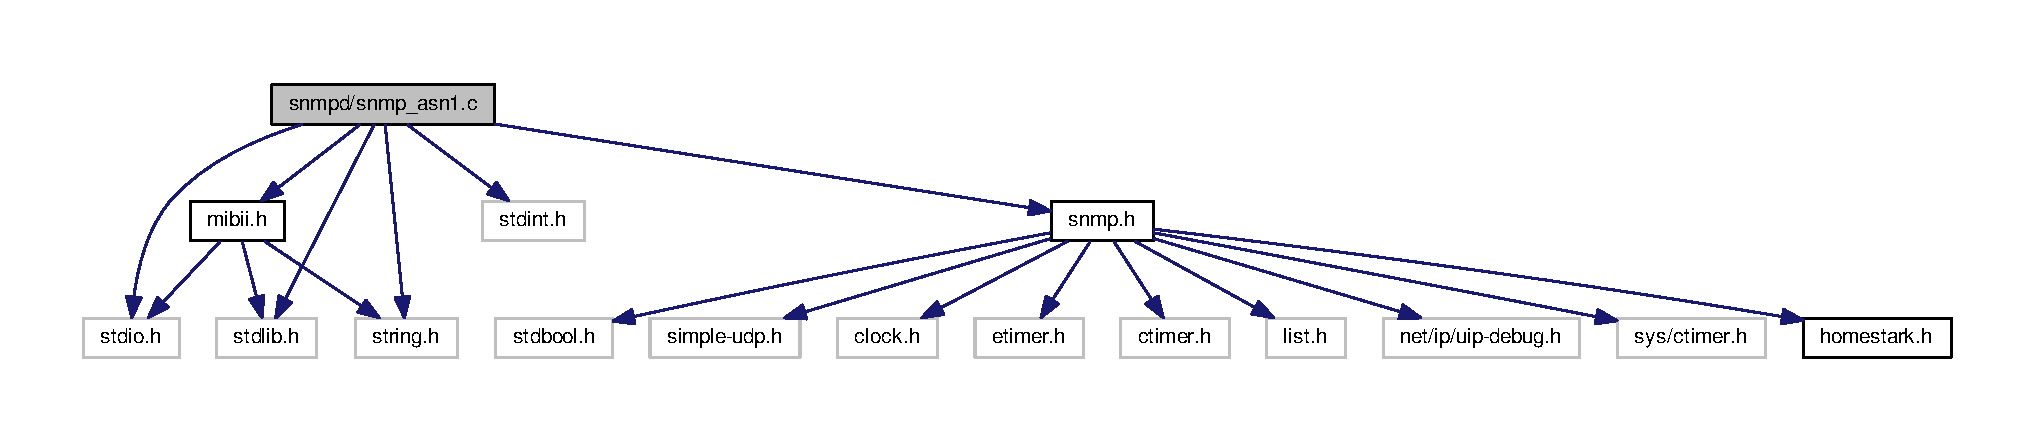
\includegraphics[width=350pt]{snmp__asn1_8c__incl}
\end{center}
\end{figure}
\subsection*{Funções}
\begin{DoxyCompactItemize}
\item 
\hypertarget{snmp__asn1_8c_a7a9e77260c38b403e735d841d860d643}{\hyperlink{snmp_8h_add91ba4199db8665b9b9fc56fc6783a6}{resp\+\_\+con\+\_\+t} {\bfseries error\+\_\+check\+\_\+snmp} (uint8\+\_\+t $\ast$error\+\_\+data)}\label{snmp__asn1_8c_a7a9e77260c38b403e735d841d860d643}

\item 
\hyperlink{snmp_8h_add91ba4199db8665b9b9fc56fc6783a6}{resp\+\_\+con\+\_\+t} \hyperlink{snmp__asn1_8c_a0c7f91118bbe8cf32398c753ead2b7f2}{decode\+\_\+asn1\+\_\+oct\+\_\+str} (uint8\+\_\+t $\ast$data\+\_\+encoded, uint8\+\_\+t $\ast$oct\+\_\+str)
\begin{DoxyCompactList}\small\item\em S\+N\+M\+P Decode Octet String. \end{DoxyCompactList}\item 
\hyperlink{snmp_8h_add91ba4199db8665b9b9fc56fc6783a6}{resp\+\_\+con\+\_\+t} \hyperlink{snmp__asn1_8c_acb3a9652e9b960748692caef7f443384}{decode\+\_\+asn1\+\_\+integer} (uint8\+\_\+t $\ast$data\+\_\+encoded, uint32\+\_\+t $\ast$integer\+\_\+value)
\begin{DoxyCompactList}\small\item\em S\+N\+M\+P Decode Integer. \end{DoxyCompactList}\item 
\hyperlink{snmp_8h_add91ba4199db8665b9b9fc56fc6783a6}{resp\+\_\+con\+\_\+t} \hyperlink{snmp__asn1_8c_af8347162889dff52c2fb4487d9a83ab3}{snmp\+\_\+decode\+\_\+message} (char $\ast$snmp\+\_\+packet, \hyperlink{structsnmp__t}{snmp\+\_\+t} $\ast$snmp\+\_\+handle)
\begin{DoxyCompactList}\small\item\em Decode S\+N\+M\+P message. \end{DoxyCompactList}\item 
uint16\+\_\+t \hyperlink{snmp__asn1_8c_a63d8ffecf9aa0af9824de046643c140f}{snmp\+\_\+encode\+\_\+message} (\hyperlink{structsnmp__t}{snmp\+\_\+t} $\ast$snmp\+\_\+handle, char $\ast$data\+\_\+encoded)
\begin{DoxyCompactList}\small\item\em Encode S\+N\+M\+P message. \end{DoxyCompactList}\item 
uint16\+\_\+t \hyperlink{snmp__asn1_8c_af72c0873252d8160ff31eae19d05a5a1}{snmp\+\_\+encode\+\_\+trap} (uint8\+\_\+t $\ast$trap\+\_\+pdu, uint8\+\_\+t type\+\_\+trap, uint8\+\_\+t heartbeat)
\begin{DoxyCompactList}\small\item\em Encode a S\+N\+M\+Pv1 Trap message. \end{DoxyCompactList}\end{DoxyCompactItemize}


\subsection{Descrição detalhada}
Licensed to the Apache Software Foundation (A\+S\+F) under one or more contributor license agreements. 

See the N\+O\+T\+I\+C\+E file distributed with this work for additional information regarding copyright ownership. The A\+S\+F licenses this file to you under the Apache License, Version 2.\+0 (the \char`\"{}\+License\char`\"{}); you may not use this file except in compliance with the License. You may obtain a copy of the License at

\href{http://www.apache.org/licenses/LICENSE-2.0}{\tt http\+://www.\+apache.\+org/licenses/\+L\+I\+C\+E\+N\+S\+E-\/2.\+0}

Unless required by applicable law or agreed to in writing, software distributed under the License is distributed on an \char`\"{}\+A\+S I\+S\char`\"{} B\+A\+S\+I\+S, W\+I\+T\+H\+O\+U\+T W\+A\+R\+R\+A\+N\+T\+I\+E\+S O\+R C\+O\+N\+D\+I\+T\+I\+O\+N\+S O\+F A\+N\+Y K\+I\+N\+D, either express or implied. See the License for the specific language governing permissions and limitations under the License.

This project is under A\+P\+A\+C\+H\+E 2.\+0 license.

Encoding and decoding functions to S\+N\+M\+P agent \begin{DoxyAuthor}{Autor}
Ânderson Ignácio da Silva 
\end{DoxyAuthor}
\begin{DoxyDate}{Data}
19 Sept 2016 
\end{DoxyDate}
\begin{DoxySeeAlso}{Veja também}
\href{http://www.aignacio.com}{\tt http\+://www.\+aignacio.\+com} 
\end{DoxySeeAlso}


\subsection{Documentação das funções}
\hypertarget{snmp__asn1_8c_acb3a9652e9b960748692caef7f443384}{\index{snmp\+\_\+asn1.\+c@{snmp\+\_\+asn1.\+c}!decode\+\_\+asn1\+\_\+integer@{decode\+\_\+asn1\+\_\+integer}}
\index{decode\+\_\+asn1\+\_\+integer@{decode\+\_\+asn1\+\_\+integer}!snmp\+\_\+asn1.\+c@{snmp\+\_\+asn1.\+c}}
\subsubsection[{decode\+\_\+asn1\+\_\+integer}]{\setlength{\rightskip}{0pt plus 5cm}{\bf resp\+\_\+con\+\_\+t} decode\+\_\+asn1\+\_\+integer (
\begin{DoxyParamCaption}
\item[{uint8\+\_\+t $\ast$}]{data\+\_\+encoded, }
\item[{uint32\+\_\+t $\ast$}]{integer\+\_\+value}
\end{DoxyParamCaption}
)}}\label{snmp__asn1_8c_acb3a9652e9b960748692caef7f443384}


S\+N\+M\+P Decode Integer. 

Decode A\+S\+N.\+1 integer(32 bit value).


\begin{DoxyParams}[1]{Parâmetros}
\mbox{\tt in}  & {\em data\+\_\+encoded} & Data do decode \\
\hline
\mbox{\tt in}  & {\em integer\+\_\+value} & Variable the will receive the integer 32-\/bit\\
\hline
\end{DoxyParams}

\begin{DoxyRetVals}{Valores retornados}
{\em S\+U\+C\+C\+E\+S\+S\+\_\+\+C\+O\+N} & Success to decode integer \\
\hline
{\em F\+A\+I\+L\+\_\+\+C\+O\+N} & Fail to decode integer \\
\hline
\end{DoxyRetVals}

\begin{DoxyCode}
91                                                                               \{
92   uint8\_t length = (intptr\_t)*(data\_encoded+1);
93   \textcolor{comment}{// uint32\_t integer\_value;}
94   \textcolor{keywordtype}{size\_t} i = 0;
95   uint32\_t aux;
96 
97   \textcolor{comment}{// Test if it's an integer value to be decoded}
98   \textcolor{keywordflow}{if} (*data\_encoded != \hyperlink{snmp_8h_a45fec4a033960bca8c60e2f40d1d0e04}{ASN1\_PRIM\_INTEGER})\{
99     debug\_snmp(\textcolor{stringliteral}{"The value is not integer!"});
100     \textcolor{keywordflow}{return} \hyperlink{snmp_8h_add91ba4199db8665b9b9fc56fc6783a6ac6ae922662cbaf7958eb387bfd6fe4da}{FAIL\_CON};
101   \}
102 
103   \textcolor{keywordflow}{for} (i=1, *integer\_value = 0; i <= length; i++)\{
104     aux = *(data\_encoded+1+i);
105     *integer\_value += aux*(pow(256,(length-i)));
106     \textcolor{comment}{// debug\_snmp("%lu * 256^%d = %lu",aux,(length-i),*integer\_value);}
107   \}
108   \textcolor{keywordflow}{return} \hyperlink{snmp_8h_add91ba4199db8665b9b9fc56fc6783a6ae7b7a388c90c2c5428cced225760885f}{SUCCESS\_CON};
109 \}
\end{DoxyCode}
\hypertarget{snmp__asn1_8c_a0c7f91118bbe8cf32398c753ead2b7f2}{\index{snmp\+\_\+asn1.\+c@{snmp\+\_\+asn1.\+c}!decode\+\_\+asn1\+\_\+oct\+\_\+str@{decode\+\_\+asn1\+\_\+oct\+\_\+str}}
\index{decode\+\_\+asn1\+\_\+oct\+\_\+str@{decode\+\_\+asn1\+\_\+oct\+\_\+str}!snmp\+\_\+asn1.\+c@{snmp\+\_\+asn1.\+c}}
\subsubsection[{decode\+\_\+asn1\+\_\+oct\+\_\+str}]{\setlength{\rightskip}{0pt plus 5cm}{\bf resp\+\_\+con\+\_\+t} decode\+\_\+asn1\+\_\+oct\+\_\+str (
\begin{DoxyParamCaption}
\item[{uint8\+\_\+t $\ast$}]{data\+\_\+encoded, }
\item[{uint8\+\_\+t $\ast$}]{oct\+\_\+str}
\end{DoxyParamCaption}
)}}\label{snmp__asn1_8c_a0c7f91118bbe8cf32398c753ead2b7f2}


S\+N\+M\+P Decode Octet String. 

Decode Octet String in A\+S\+N.\+1 format.


\begin{DoxyParams}[1]{Parâmetros}
\mbox{\tt in}  & {\em data\+\_\+encoded} & Data do decode \\
\hline
\mbox{\tt in}  & {\em oct\+\_\+str} & Variable the will receive the octet string\\
\hline
\end{DoxyParams}

\begin{DoxyRetVals}{Valores retornados}
{\em S\+U\+C\+C\+E\+S\+S\+\_\+\+C\+O\+N} & Success to decode string octet \\
\hline
{\em F\+A\+I\+L\+\_\+\+C\+O\+N} & Fail to decode octet string \\
\hline
\end{DoxyRetVals}

\begin{DoxyCode}
72                                                                        \{
73   \textcolor{keywordflow}{if} (*data\_encoded !=  (intptr\_t)ASN1\_PRIM\_OCT\_STR) \{
74     debug\_snmp(\textcolor{stringliteral}{"The type of value passed is not an octet string!"});
75     \textcolor{keywordflow}{return} \hyperlink{snmp_8h_add91ba4199db8665b9b9fc56fc6783a6ac6ae922662cbaf7958eb387bfd6fe4da}{FAIL\_CON};
76   \}
77 
78   uint8\_t length = (intptr\_t)*(data\_encoded+1),
79           index = 0;
80   \textcolor{keywordflow}{while} (length) \{
81     *(oct\_str+index) = (intptr\_t)*(data\_encoded+2+index);
82     length--;
83     index++;
84   \}
85 
86   *(oct\_str+index) = \textcolor{charliteral}{'\(\backslash\)0'};
87   \textcolor{comment}{// printf("\(\backslash\)nEndereco----:> %d\(\backslash\)n",oct\_str);}
88   \textcolor{keywordflow}{return} \hyperlink{snmp_8h_add91ba4199db8665b9b9fc56fc6783a6ae7b7a388c90c2c5428cced225760885f}{SUCCESS\_CON};
89 \}
\end{DoxyCode}
\hypertarget{snmp__asn1_8c_af8347162889dff52c2fb4487d9a83ab3}{\index{snmp\+\_\+asn1.\+c@{snmp\+\_\+asn1.\+c}!snmp\+\_\+decode\+\_\+message@{snmp\+\_\+decode\+\_\+message}}
\index{snmp\+\_\+decode\+\_\+message@{snmp\+\_\+decode\+\_\+message}!snmp\+\_\+asn1.\+c@{snmp\+\_\+asn1.\+c}}
\subsubsection[{snmp\+\_\+decode\+\_\+message}]{\setlength{\rightskip}{0pt plus 5cm}{\bf resp\+\_\+con\+\_\+t} snmp\+\_\+decode\+\_\+message (
\begin{DoxyParamCaption}
\item[{char $\ast$}]{snmp\+\_\+packet, }
\item[{{\bf snmp\+\_\+t} $\ast$}]{v}
\end{DoxyParamCaption}
)}}\label{snmp__asn1_8c_af8347162889dff52c2fb4487d9a83ab3}


Decode S\+N\+M\+P message. 

Decode a S\+N\+M\+P message v1 and format to answer request.


\begin{DoxyParams}[1]{Parâmetros}
\mbox{\tt in}  & {\em snmp\+\_\+packet} & Data U\+D\+P -\/ S\+N\+M\+P to decode \\
\hline
\mbox{\tt in}  & {\em snmp\+\_\+handle} & Struct that will receive the S\+N\+M\+P request messsage\\
\hline
\end{DoxyParams}

\begin{DoxyRetVals}{Valores retornados}
{\em S\+U\+C\+C\+E\+S\+S\+\_\+\+C\+O\+N} & Success to decode S\+N\+M\+P Message \\
\hline
{\em F\+A\+I\+L\+\_\+\+C\+O\+N} & Fail to decode S\+N\+M\+P Message \\
\hline
\end{DoxyRetVals}

\begin{DoxyCode}
111                                                                       \{
112   uint8\_t buffer[50], aux;
113   \textcolor{keywordtype}{size\_t} i;
114 
115 \textcolor{preprocessor}{  #ifdef DEBUG\_SNMP\_DECODING}
116   \textcolor{comment}{// debug\_snmp("Encoded SNMP packet:\(\backslash\)n\(\backslash\)t");}
117   \textcolor{comment}{// for (i=0, j=0; i < *(snmp\_packet+1)+1; j++, i++)\{}
118   \textcolor{comment}{//   if (j > 7)\{}
119   \textcolor{comment}{//     j = 0;}
120   \textcolor{comment}{//     printf("\(\backslash\)n\(\backslash\)t");}
121   \textcolor{comment}{//   \}}
122   \textcolor{comment}{//   printf("[%02x] ",*(snmp\_packet+i));}
123   \textcolor{comment}{// \}}
124 \textcolor{preprocessor}{  #endif}
125 
126   \textcolor{keywordflow}{if} (!\hyperlink{snmp_8h_a388ebedb8b344492bded4ba233fab27d}{check\_seq}(*snmp\_packet))\{
127     debug\_snmp(\textcolor{stringliteral}{"Sequence initial of SNMP message error:%x"},*snmp\_packet);
128     \textcolor{keywordflow}{return} \hyperlink{snmp_8h_add91ba4199db8665b9b9fc56fc6783a6ac6ae922662cbaf7958eb387bfd6fe4da}{FAIL\_CON};
129   \}
130 
131   \textcolor{comment}{/************************ Check the SNMP version ****************************/}
132   \textcolor{keywordflow}{for} (i=0;i < *(snmp\_packet+3)+2; i++)
133     buffer[i] = *(snmp\_packet+2+i);
134   uint32\_t SNMPv = 0;
135   \textcolor{keywordflow}{if} (!\hyperlink{snmp__asn1_8c_acb3a9652e9b960748692caef7f443384}{decode\_asn1\_integer}(buffer,&SNMPv)) \textcolor{keywordflow}{return} \hyperlink{snmp_8h_add91ba4199db8665b9b9fc56fc6783a6ac6ae922662cbaf7958eb387bfd6fe4da}{FAIL\_CON};
136 \textcolor{preprocessor}{  #ifdef DEBUG\_SNMP\_DECODING}
137   debug\_snmp(\textcolor{stringliteral}{"Version SNMP:[1] OK"});
138 \textcolor{preprocessor}{  #endif}
139   \textcolor{keywordflow}{if} (SNMPv != \hyperlink{snmp_8h_a1f1b7fadcf29f1de5bb406bf356c1d71}{SNMP\_VERSION\_1}) \{
140     debug\_snmp(\textcolor{stringliteral}{"SNMP version is different from v1:%lu"},SNMPv);
141     \textcolor{keywordflow}{return} \hyperlink{snmp_8h_add91ba4199db8665b9b9fc56fc6783a6ac6ae922662cbaf7958eb387bfd6fe4da}{FAIL\_CON};
142   \}
143   snmp\_handle->snmp\_version = SNMPv;
144 
145   \textcolor{comment}{/********************** Get the community string ****************************/}
146   \textcolor{keywordflow}{for} (i=0;i < *(snmp\_packet+6)+2; i++)
147   snmp\_handle->community[i] = *(snmp\_packet+5+i);
148   snmp\_handle->community[i] = \textcolor{charliteral}{'\(\backslash\)0'};
149   aux = i;
150 \textcolor{preprocessor}{  #ifdef DEBUG\_SNMP\_DECODING}
151   debug\_snmp(\textcolor{stringliteral}{"Community String: "});
152   \textcolor{keywordflow}{for} (i=0; i < aux; i++)\{
153     \textcolor{keywordflow}{if} (i<2)
154       printf(\textcolor{stringliteral}{"[%d]"},snmp\_handle->community[i]);
155     \textcolor{keywordflow}{else}
156       printf(\textcolor{stringliteral}{"[%c]"},snmp\_handle->community[i]);
157   \}
158 \textcolor{preprocessor}{  #endif}
159 
160   \textcolor{comment}{/************************** Get the request ID ******************************/}
161   aux = 5+snmp\_handle->community[1]+2+2;
162   \textcolor{keywordflow}{for} (i=0;i < *(snmp\_packet+aux+1)+2; i++)
163     snmp\_handle->request\_id\_c[i] = *(snmp\_packet+aux+i);
164   snmp\_handle->request\_id\_c[i] = \textcolor{charliteral}{'\(\backslash\)0'};
165   aux = i;
166 \textcolor{preprocessor}{  #ifdef DEBUG\_SNMP\_DECODING}
167   debug\_snmp(\textcolor{stringliteral}{"Request ID: "});
168   \textcolor{keywordflow}{for} (i=0; i < aux; i++)\{
169     \textcolor{keywordflow}{if} (i<2)
170       printf(\textcolor{stringliteral}{"[%d]"},snmp\_handle->request\_id\_c[i]);
171     \textcolor{keywordflow}{else}
172     printf(\textcolor{stringliteral}{"[%x]"},snmp\_handle->request\_id\_c[i]);
173   \}
174 \textcolor{preprocessor}{  #endif}
175 
176   \textcolor{comment}{/************************** Check for errors ********************************/}
177   aux = 5+(snmp\_handle->community[1]+2)+2+(snmp\_handle->request\_id\_c[1]+2);
178   \textcolor{keywordflow}{for} (i=0;i < 6; i++)
179     buffer[i] = *(snmp\_packet+aux+i);
180   buffer[i] = \textcolor{charliteral}{'\(\backslash\)0'};
181   error\_check\_snmp(buffer);
182 
183   \textcolor{comment}{/**************************** Get the OID ***********************************/}
184   aux = 5+(snmp\_handle->community[1]+2);
185   aux += 2+(snmp\_handle->request\_id\_c[1]+2)+10;
186   \textcolor{keywordflow}{for} (i=0;i < *(snmp\_packet+aux+1)+2; i++)
187     snmp\_handle->oid\_encoded[i] = *(snmp\_packet+aux+i);
188   snmp\_handle->oid\_encoded[i] = \textcolor{charliteral}{'\(\backslash\)0'};
189   aux = i;
190 \textcolor{preprocessor}{  #ifdef DEBUG\_SNMP\_DECODING}
191   debug\_snmp(\textcolor{stringliteral}{"OID: "});
192   \textcolor{keywordflow}{for} (i=0; i < aux; i++)\{
193     \textcolor{keywordflow}{if} (i <= 1)
194       printf(\textcolor{stringliteral}{"[%d]"},snmp\_handle->oid\_encoded[i]);
195     \textcolor{keywordflow}{else} \textcolor{keywordflow}{if} (i == 2)
196       printf(\textcolor{stringliteral}{"[%d."},snmp\_handle->oid\_encoded[i]);
197     \textcolor{keywordflow}{else}
198     printf(\textcolor{stringliteral}{"%d."},snmp\_handle->oid\_encoded[i]);
199   \}
200   printf(\textcolor{stringliteral}{"]"});
201 \textcolor{preprocessor}{  #endif}
202 
203   \textcolor{comment}{/************************** Get the PDU type ********************************/}
204   aux = 5+(snmp\_handle->community[1]+2);
205   snmp\_handle->request\_type  = *(snmp\_packet+aux);
206   snmp\_handle->response\_type = ASN1\_CPX\_GET\_RESP;
207 
208   uint8\_t string\_value[\hyperlink{snmp_8h_a23bdc4d15d908a80e4bc06be55463ffc}{MAX\_OCTET\_STRING}];
209   uint8\_t status\_mib2 = \hyperlink{mibii_8c_aa0bb802c0b80aaab6218e5a7753f8e28}{mib\_ii\_get\_oid}(snmp\_handle->oid\_encoded,&string\_value[0]);
210 
211   \textcolor{keywordflow}{switch} (snmp\_handle->request\_type) \{
212     \textcolor{keywordflow}{case} \hyperlink{snmp_8h_aa4d923102cb2314e31cbf833482e9090}{ASN1\_CPX\_SEQUENCE}:
213     \textcolor{keywordflow}{break};
214     \textcolor{keywordflow}{case} ASN1\_CPX\_GET\_REQ:
215       aux = snmp\_handle->oid\_encoded[1]+1;
216       \textcolor{keywordflow}{if} (snmp\_handle->oid\_encoded[aux] != 0   ||
217           snmp\_handle->oid\_encoded[aux-3] != 1 ||
218           snmp\_handle->oid\_encoded[aux-4] != 2 ||
219           snmp\_handle->oid\_encoded[aux-5] != 1 ||
220           snmp\_handle->oid\_encoded[aux-6] != 6 ||
221           snmp\_handle->oid\_encoded[aux-7] != 0x2b)\{
222         snmp\_handle->oid\_encoded[aux] = 1;
223         status\_mib2 = \hyperlink{mibii_8c_aa0bb802c0b80aaab6218e5a7753f8e28}{mib\_ii\_get\_oid}(snmp\_handle->oid\_encoded,&string\_value[0]);
224       \}
225 \textcolor{preprocessor}{      #ifdef DEBUG\_SNMP\_DECODING}
226       debug\_snmp(\textcolor{stringliteral}{"GET Request PDU Type"});
227 \textcolor{preprocessor}{      #endif}
228       \textcolor{keywordflow}{if} (!status\_mib2)\{
229 \textcolor{preprocessor}{        #ifdef DEBUG\_SNMP\_DECODING}
230         debug\_snmp(\textcolor{stringliteral}{"There isn't an value for that OID!"});
231 \textcolor{preprocessor}{        #endif}
232         snmp\_handle->value[0] = 0x05;
233         snmp\_handle->value[1] = 0x00;
234       \}
235       \textcolor{keywordflow}{else} \{
236         aux = strlen((\textcolor{keyword}{const} \textcolor{keywordtype}{char}*)string\_value);
237         snmp\_handle->value[0] = ASN1\_PRIM\_OCT\_STR;
238         snmp\_handle->value[1] = aux;
239 
240         \textcolor{keywordflow}{for} (i = 0; i < aux; i++)
241           snmp\_handle->value[2+i] = string\_value[i];
242         #ifdef DEBUG\_SNMP\_DECODING
243         debug\_snmp(\textcolor{stringliteral}{"String for OID: "});
244         \textcolor{keywordflow}{for} (i=0; i < aux+2; i++)\{
245           \textcolor{keywordflow}{if} (i == 0)
246             printf(\textcolor{stringliteral}{"[%x]"},snmp\_handle->value[i]);
247           \textcolor{keywordflow}{else} \textcolor{keywordflow}{if} (i == 1)
248             printf(\textcolor{stringliteral}{"[%d]["},snmp\_handle->value[i]);
249           \textcolor{keywordflow}{else}
250             printf(\textcolor{stringliteral}{"%c"},snmp\_handle->value[i]);
251         \}
252         printf(\textcolor{stringliteral}{"]"});
253 \textcolor{preprocessor}{        #endif}
254       \}
255     \textcolor{keywordflow}{break};
256     \textcolor{keywordflow}{case} ASN1\_CPX\_NEXT\_REQ:
257       \textcolor{comment}{// Let's check the last byte}
258       aux = snmp\_handle->oid\_encoded[1]+1;
259       \textcolor{keywordflow}{if} (snmp\_handle->oid\_encoded[aux] == 0) \{
260         \textcolor{comment}{// We need to increment the OID for the snmpwalk... requisition}
261         \textcolor{keywordflow}{if} (snmp\_handle->oid\_encoded[aux-1] < 9) \{
262           snmp\_handle->oid\_encoded[aux-1] = snmp\_handle->oid\_encoded[aux-1]+1;
263         \}
264         \textcolor{keywordflow}{else}
265           snmp\_handle->oid\_encoded[aux] = 1; \textcolor{comment}{// Let's force not unknow value in the mib tree}
266         status\_mib2 = \hyperlink{mibii_8c_aa0bb802c0b80aaab6218e5a7753f8e28}{mib\_ii\_get\_oid}(snmp\_handle->oid\_encoded,&string\_value[0]);
267       \}
268       \textcolor{keywordflow}{else}\{
269         \textcolor{keywordflow}{if} (snmp\_handle->oid\_encoded[aux-1] == 1 &&
270             snmp\_handle->oid\_encoded[aux-2] == 2 &&
271             snmp\_handle->oid\_encoded[aux-3] == 1 &&
272             snmp\_handle->oid\_encoded[aux-4] == 6 &&
273             snmp\_handle->oid\_encoded[aux-5] == 0x2b) \{
274           snmp\_handle->oid\_encoded[1] += 2;
275           snmp\_handle->oid\_encoded[aux+1] = 1;
276           snmp\_handle->oid\_encoded[aux+2] = 0;
277           snmp\_handle->oid\_encoded[aux+3] = \textcolor{charliteral}{'\(\backslash\)0'};
278         \}
279         \textcolor{comment}{// We need to set to the nearest OID for the snmpwalk... requisition, in this case .1.0}
280         status\_mib2 = \hyperlink{mibii_8c_aa0bb802c0b80aaab6218e5a7753f8e28}{mib\_ii\_get\_oid}(snmp\_handle->oid\_encoded,&string\_value[0]);
281       \}
282 
283 \textcolor{preprocessor}{      #ifdef DEBUG\_SNMP\_DECODING}
284       debug\_snmp(\textcolor{stringliteral}{"GET NEXT Request PDU Type"});
285 \textcolor{preprocessor}{      #endif}
286       \textcolor{keywordflow}{if} (!status\_mib2)\{
287 \textcolor{preprocessor}{        #ifdef DEBUG\_SNMP\_DECODING}
288         debug\_snmp(\textcolor{stringliteral}{"There isn't an value for that OID!"});
289 \textcolor{preprocessor}{        #endif}
290         snmp\_handle->value[0] = 0x05;
291         snmp\_handle->value[1] = 0x00;
292       \}
293       \textcolor{keywordflow}{else} \{
294         aux = strlen((\textcolor{keyword}{const} \textcolor{keywordtype}{char}*)string\_value);
295         snmp\_handle->value[0] = ASN1\_PRIM\_OCT\_STR;
296         snmp\_handle->value[1] = aux;
297 
298         \textcolor{keywordflow}{for} (i = 0; i < aux; i++)
299           snmp\_handle->value[2+i] = string\_value[i];
300         #ifdef DEBUG\_SNMP\_DECODING
301         debug\_snmp(\textcolor{stringliteral}{"String for OID: "});
302         \textcolor{keywordflow}{for} (i=0; i < aux+2; i++)\{
303           \textcolor{keywordflow}{if} (i == 0)
304             printf(\textcolor{stringliteral}{"[%x]"},snmp\_handle->value[i]);
305           \textcolor{keywordflow}{else} \textcolor{keywordflow}{if} (i == 1)
306             printf(\textcolor{stringliteral}{"[%d]["},snmp\_handle->value[i]);
307           \textcolor{keywordflow}{else}
308             printf(\textcolor{stringliteral}{"%c"},snmp\_handle->value[i]);
309         \}
310         printf(\textcolor{stringliteral}{"]"});
311 \textcolor{preprocessor}{        #endif}
312       \}
313     \textcolor{keywordflow}{break};
314     \textcolor{keywordflow}{case} ASN1\_CPX\_GET\_RESP:
315     \textcolor{keywordflow}{break};
316     \textcolor{keywordflow}{case} ASN1\_CPX\_SET\_REQ:
317     \textcolor{keywordflow}{break};
318     \textcolor{keywordflow}{default}:
319 \textcolor{preprocessor}{      #ifdef DEBUG\_SNMP\_DECODING}
320       debug\_snmp(\textcolor{stringliteral}{"The PDU type is not know"});
321 \textcolor{preprocessor}{      #endif}
322       \textcolor{keywordflow}{return} \hyperlink{snmp_8h_add91ba4199db8665b9b9fc56fc6783a6ac6ae922662cbaf7958eb387bfd6fe4da}{FAIL\_CON};
323     \textcolor{keywordflow}{break};
324   \}
325 
326 \textcolor{preprocessor}{  #ifdef DEBUG\_SNMP\_DECODING}
327   printf(\textcolor{stringliteral}{"\(\backslash\)n"});
328 \textcolor{preprocessor}{  #endif}
329   \textcolor{keywordflow}{return} \hyperlink{snmp_8h_add91ba4199db8665b9b9fc56fc6783a6ae7b7a388c90c2c5428cced225760885f}{SUCCESS\_CON};
330 \}
\end{DoxyCode}
\hypertarget{snmp__asn1_8c_a63d8ffecf9aa0af9824de046643c140f}{\index{snmp\+\_\+asn1.\+c@{snmp\+\_\+asn1.\+c}!snmp\+\_\+encode\+\_\+message@{snmp\+\_\+encode\+\_\+message}}
\index{snmp\+\_\+encode\+\_\+message@{snmp\+\_\+encode\+\_\+message}!snmp\+\_\+asn1.\+c@{snmp\+\_\+asn1.\+c}}
\subsubsection[{snmp\+\_\+encode\+\_\+message}]{\setlength{\rightskip}{0pt plus 5cm}uint16\+\_\+t snmp\+\_\+encode\+\_\+message (
\begin{DoxyParamCaption}
\item[{{\bf snmp\+\_\+t} $\ast$}]{snmp\+\_\+handle, }
\item[{char $\ast$}]{data\+\_\+encoded}
\end{DoxyParamCaption}
)}}\label{snmp__asn1_8c_a63d8ffecf9aa0af9824de046643c140f}


Encode S\+N\+M\+P message. 

Encode a S\+N\+M\+P message and format to send the answer.


\begin{DoxyParams}[1]{Parâmetros}
\mbox{\tt in}  & {\em snmp\+\_\+handle} & Struct that will be encoded in the S\+N\+M\+P message format \\
\hline
\mbox{\tt in}  & {\em data\+\_\+encoded} & Variable that'll receive the encoded S\+N\+M\+P Message\\
\hline
\end{DoxyParams}

\begin{DoxyRetVals}{Valores retornados}
{\em length} & Length of U\+D\+P packet encoded \\
\hline
\end{DoxyRetVals}

\begin{DoxyCode}
332                                                                      \{
333   uint8\_t i, aux = 0, aux2 = 0;
334   *data\_encoded = \hyperlink{snmp_8h_aa4d923102cb2314e31cbf833482e9090}{ASN1\_CPX\_SEQUENCE};
335 
336   aux2 = 0;
337   aux2 += 3+(snmp\_handle->community[1]+2)+12;
338   aux2 += (snmp\_handle->request\_id\_c[1]+2);
339   aux2 += (snmp\_handle->oid\_encoded[1]+2);
340   aux2 += (snmp\_handle->value[1]+2);
341   *(data\_encoded+1) = aux2;
342 
343   *(data\_encoded+2) = \hyperlink{snmp_8h_a45fec4a033960bca8c60e2f40d1d0e04}{ASN1\_PRIM\_INTEGER};
344   *(data\_encoded+3) = 0x01;
345   \textcolor{keywordflow}{switch} (snmp\_handle->snmp\_version) \{
346     \textcolor{keywordflow}{case} \hyperlink{snmp_8h_a1f1b7fadcf29f1de5bb406bf356c1d71}{SNMP\_VERSION\_1}:
347       *(data\_encoded+4) = \hyperlink{snmp_8h_a1f1b7fadcf29f1de5bb406bf356c1d71}{SNMP\_VERSION\_1};
348     \textcolor{keywordflow}{break};
349     \textcolor{keywordflow}{case} \hyperlink{snmp_8h_a0599530b4b198b2c7fa49a274f3f3878}{SNMP\_VERSION\_2C}:
350       *(data\_encoded+4) = \hyperlink{snmp_8h_a0599530b4b198b2c7fa49a274f3f3878}{SNMP\_VERSION\_2C};
351     \textcolor{keywordflow}{break};
352     \textcolor{keywordflow}{case} \hyperlink{snmp_8h_aa0b283beac3c7da5c28058f52a817c0c}{SNMP\_VERSION\_3}:
353       *(data\_encoded+4) = \hyperlink{snmp_8h_aa0b283beac3c7da5c28058f52a817c0c}{SNMP\_VERSION\_3};
354     \textcolor{keywordflow}{break};
355     \textcolor{keywordflow}{default}:
356       debug\_snmp(\textcolor{stringliteral}{"Version SNMP not supported"});
357       \textcolor{keywordflow}{return} \hyperlink{snmp_8h_add91ba4199db8665b9b9fc56fc6783a6ac6ae922662cbaf7958eb387bfd6fe4da}{FAIL\_CON};
358     \textcolor{keywordflow}{break};
359   \}
360 
361   \textcolor{keywordflow}{for} ( i = 0; i < snmp\_handle->community[1]+2; i++)
362     *(data\_encoded+5+i) = snmp\_handle->community[i];
363 
364   aux = 5+snmp\_handle->community[1]+2;
365   *(data\_encoded+aux) = ASN1\_CPX\_GET\_RESP;
366 
367   aux2 = 0;
368   aux2 += (snmp\_handle->request\_id\_c[1]+2)+10;
369   aux2 += (snmp\_handle->oid\_encoded[1]+2);
370   aux2 += (snmp\_handle->value[1]+2);
371   *(data\_encoded+aux+1) = aux2;
372 
373   aux += 2;
374   \textcolor{keywordflow}{for} ( i = 0; i < snmp\_handle->request\_id\_c[1]+2; i++)
375     *(data\_encoded+aux+i) = snmp\_handle->request\_id\_c[i];
376 
377   aux += snmp\_handle->request\_id\_c[1]+2;
378 
379   \textcolor{keywordflow}{if} (snmp\_handle->value[0] == ASN1\_PRIM\_NULL) \{
380     *(data\_encoded+aux) = \hyperlink{snmp_8h_a45fec4a033960bca8c60e2f40d1d0e04}{ASN1\_PRIM\_INTEGER};
381     aux++;
382     *(data\_encoded+aux) = 0x01;
383     aux++;
384     *(data\_encoded+aux) = ERROR\_REQ\_OID\_NOT\_FOUND;
385     aux++;
386     *(data\_encoded+aux) = \hyperlink{snmp_8h_a45fec4a033960bca8c60e2f40d1d0e04}{ASN1\_PRIM\_INTEGER};
387     aux++;
388     *(data\_encoded+aux) = 0x01;
389     aux++;
390     *(data\_encoded+aux) = ERROR\_RESP\_TOO\_LARGE;
391     aux++;
392     *(data\_encoded+aux) = \hyperlink{snmp_8h_aa4d923102cb2314e31cbf833482e9090}{ASN1\_CPX\_SEQUENCE};
393     aux++;
394     aux2 = 2;
395     aux2 += (snmp\_handle->oid\_encoded[1]+2);
396     aux2 += (snmp\_handle->value[1]+2);
397     *(data\_encoded+aux) = aux2;
398     aux++;
399     *(data\_encoded+aux) = \hyperlink{snmp_8h_aa4d923102cb2314e31cbf833482e9090}{ASN1\_CPX\_SEQUENCE};
400     aux++;
401     aux2 = 0;
402     aux2 += (snmp\_handle->oid\_encoded[1]+2);
403     aux2 += (snmp\_handle->value[1]+2);
404     *(data\_encoded+aux) = aux2;
405     aux++;
406     \textcolor{keywordflow}{for} ( i = 0; i < snmp\_handle->oid\_encoded[1]+2; i++)
407       *(data\_encoded+aux+i) = snmp\_handle->oid\_encoded[i];
408     aux += snmp\_handle->oid\_encoded[1]+2;
409     *(data\_encoded+aux) = ASN1\_PRIM\_NULL;
410     aux++;
411     *(data\_encoded+aux) = 0x00;
412   \}
413   \textcolor{keywordflow}{else}\{
414     *(data\_encoded+aux) = \hyperlink{snmp_8h_a45fec4a033960bca8c60e2f40d1d0e04}{ASN1\_PRIM\_INTEGER};
415     aux++;
416     *(data\_encoded+aux) = 0x01;
417     aux++;
418     *(data\_encoded+aux) = \hyperlink{snmp_8h_abe670cc5ceed3fad3be682fc0c1bb62e}{ERROR\_NONE};
419     aux++;
420     *(data\_encoded+aux) = \hyperlink{snmp_8h_a45fec4a033960bca8c60e2f40d1d0e04}{ASN1\_PRIM\_INTEGER};
421     aux++;
422     *(data\_encoded+aux) = 0x01;
423     aux++;
424     *(data\_encoded+aux) = \hyperlink{snmp_8h_abe670cc5ceed3fad3be682fc0c1bb62e}{ERROR\_NONE};
425     aux++;
426     *(data\_encoded+aux) = \hyperlink{snmp_8h_aa4d923102cb2314e31cbf833482e9090}{ASN1\_CPX\_SEQUENCE};
427     aux++;
428     aux2 = 2;
429     aux2 += (snmp\_handle->oid\_encoded[1]+2);
430     aux2 += (snmp\_handle->value[1]+2);
431     *(data\_encoded+aux) = aux2;
432     aux++;
433     *(data\_encoded+aux) = \hyperlink{snmp_8h_aa4d923102cb2314e31cbf833482e9090}{ASN1\_CPX\_SEQUENCE};
434     aux++;
435     aux2 = 0;
436     aux2 += (snmp\_handle->oid\_encoded[1]+2);
437     aux2 += (snmp\_handle->value[1]+2);
438     *(data\_encoded+aux) = aux2;
439     aux++;
440     \textcolor{keywordflow}{for} ( i = 0; i < snmp\_handle->oid\_encoded[1]+2; i++)
441       *(data\_encoded+aux+i) = snmp\_handle->oid\_encoded[i];
442     aux += snmp\_handle->oid\_encoded[1]+2;
443     \textcolor{keywordflow}{for} ( i = 0; i < snmp\_handle->value[1]+2; i++)
444       *(data\_encoded+aux+i) = snmp\_handle->value[i];
445   \}
446 \textcolor{preprocessor}{  #ifdef DEBUG\_SNMP\_DECODING}
447   debug\_snmp(\textcolor{stringliteral}{"Len of encoded packet: %d"},*(data\_encoded+1)+1);
448 \textcolor{preprocessor}{  #endif}
449   \textcolor{keywordflow}{return} *(data\_encoded+1)+2;
450 \}
\end{DoxyCode}
\hypertarget{snmp__asn1_8c_af72c0873252d8160ff31eae19d05a5a1}{\index{snmp\+\_\+asn1.\+c@{snmp\+\_\+asn1.\+c}!snmp\+\_\+encode\+\_\+trap@{snmp\+\_\+encode\+\_\+trap}}
\index{snmp\+\_\+encode\+\_\+trap@{snmp\+\_\+encode\+\_\+trap}!snmp\+\_\+asn1.\+c@{snmp\+\_\+asn1.\+c}}
\subsubsection[{snmp\+\_\+encode\+\_\+trap}]{\setlength{\rightskip}{0pt plus 5cm}uint16\+\_\+t snmp\+\_\+encode\+\_\+trap (
\begin{DoxyParamCaption}
\item[{uint8\+\_\+t $\ast$}]{trap\+\_\+pdu, }
\item[{uint8\+\_\+t}]{type\+\_\+trap, }
\item[{uint8\+\_\+t}]{heartbeat}
\end{DoxyParamCaption}
)}}\label{snmp__asn1_8c_af72c0873252d8160ff31eae19d05a5a1}


Encode a S\+N\+M\+Pv1 Trap message. 

Encode a S\+N\+M\+Pv1 Trap type message with A\+W\+G\+E\+S P\+E\+N and heartbeat value


\begin{DoxyParams}[1]{Parâmetros}
\mbox{\tt in}  & {\em trap\+\_\+pdu} & Variable that'll receive the packet encoded \\
\hline
\mbox{\tt in}  & {\em type\+\_\+trap} & Type of trap that'll send (\char`\"{}cold\+Start\char`\"{},\char`\"{}\+Warm\+Start\char`\"{}...) \\
\hline
\mbox{\tt in}  & {\em heartbeat} & Heartbeat value of the node\\
\hline
\end{DoxyParams}

\begin{DoxyRetVals}{Valores retornados}
{\em len} & Length of encoded packet \\
\hline
\end{DoxyRetVals}

\begin{DoxyCode}
483                                                                                   \{
484   \textcolor{comment}{// uint8\_t i;//, aux = 0, aux2 = 0;}
485   uint16\_t length\_trap = 0, aux = 0;
486 
487   *trap\_pdu = \hyperlink{snmp_8h_aa4d923102cb2314e31cbf833482e9090}{ASN1\_CPX\_SEQUENCE};
488   *(trap\_pdu+1) = 52+4;
489 
490   \textcolor{comment}{// SNMP Version}
491   *(trap\_pdu+2) = \hyperlink{snmp_8h_a45fec4a033960bca8c60e2f40d1d0e04}{ASN1\_PRIM\_INTEGER};
492   *(trap\_pdu+3) = 0x01;
493   *(trap\_pdu+4) = \hyperlink{snmp_8h_a1f1b7fadcf29f1de5bb406bf356c1d71}{SNMP\_VERSION\_1};
494 
495   \textcolor{comment}{// Comunity String - always "public"}
496   *(trap\_pdu+5) = ASN1\_PRIM\_OCT\_STR;
497   *(trap\_pdu+6) = 0x06;
498   *(trap\_pdu+7) = 0x70;
499   *(trap\_pdu+8) = 0x75;
500   *(trap\_pdu+9) = 0x62;
501   *(trap\_pdu+10) = 0x6c;
502   *(trap\_pdu+11) = 0x69;
503   *(trap\_pdu+12) = 0x63;
504 
505   \textcolor{comment}{// Type of PDU - Trap(0xa4)}
506   *(trap\_pdu+13) = ASN1\_CPX\_TRAP;
507   aux = 14;
508   *(trap\_pdu+aux) = 39+4;
509 
510   \textcolor{comment}{// Enterprise OID - 0x06, 0x09, 0x2b, 0x06, 0x01, 0x04, 0x01, 0x04, 0x01, 0x02, 0x15}
511   aux++;
512   *(trap\_pdu+aux) = ASN1\_PRIM\_OID;
513   aux++;
514   *(trap\_pdu+aux) = 0x09;
515   aux++;
516   *(trap\_pdu+aux) = 0x2b;
517   aux++;
518   *(trap\_pdu+aux) = 0x06;
519   aux++;
520   *(trap\_pdu+aux) = 0x01;
521   aux++;
522   *(trap\_pdu+aux) = 0x04;
523   aux++;
524   *(trap\_pdu+aux) = 0x01;
525   aux++;
526   *(trap\_pdu+aux) = 0x04;
527   aux++;
528   *(trap\_pdu+aux) = 0x01;
529   aux++;
530   *(trap\_pdu+aux) = 0x02;
531   aux++;
532   *(trap\_pdu+aux) = 0x15;
533 
534   \textcolor{comment}{// IP Address of the agent, always 0.0.0.0 if we cannot send IPv6 in SNMPv1, in SNMPv2 the trap calls
       inform}
535   aux++;
536   *(trap\_pdu+aux) = ASN1\_PRIM\_IP\_ADDRESS;
537   aux++;
538   *(trap\_pdu+aux) = 4;
539   aux++;
540   *(trap\_pdu+aux) = 0;
541   aux++;
542   *(trap\_pdu+aux) = 0;
543   aux++;
544   *(trap\_pdu+aux) = 0;
545   aux++;
546   *(trap\_pdu+aux) = 0;
547 
548   \textcolor{comment}{// Generic Trap type}
549   aux++;
550   *(trap\_pdu+aux) = \hyperlink{snmp_8h_a45fec4a033960bca8c60e2f40d1d0e04}{ASN1\_PRIM\_INTEGER};
551   aux++;
552   *(trap\_pdu+aux) = 0x01;
553   aux++;
554   *(trap\_pdu+aux) = type\_trap;
555 
556   \textcolor{comment}{// Specific Trap Number - we don't use this}
557   aux++;
558   *(trap\_pdu+aux) = \hyperlink{snmp_8h_a45fec4a033960bca8c60e2f40d1d0e04}{ASN1\_PRIM\_INTEGER};
559   aux++;
560   *(trap\_pdu+aux) = 0x01;
561   aux++;
562   *(trap\_pdu+aux) = 0x00;
563 
564   \textcolor{comment}{// Timestamp - we don't use this - default(0)}
565   aux++;
566   *(trap\_pdu+aux) = ASN1\_PRIM\_TIMESTAMP;
567   aux++;
568   *(trap\_pdu+aux) = 0x01;
569   aux++;
570   *(trap\_pdu+aux) = 0x00;
571 
572   \textcolor{comment}{// VarBind List - we don't use this - default(0)}
573   aux++;
574   *(trap\_pdu+aux) = \hyperlink{snmp_8h_aa4d923102cb2314e31cbf833482e9090}{ASN1\_CPX\_SEQUENCE};
575   aux++;
576   *(trap\_pdu+aux) = 3+8+2+2;
577 
578   \textcolor{comment}{// VarBind List - we don't use this - default(0)}
579   aux++;
580   *(trap\_pdu+aux) = \hyperlink{snmp_8h_aa4d923102cb2314e31cbf833482e9090}{ASN1\_CPX\_SEQUENCE};
581   aux++;
582   *(trap\_pdu+aux) = 3+8+2;
583 
584   \textcolor{comment}{// OID}
585   aux++;
586   *(trap\_pdu+aux) = ASN1\_PRIM\_OID;
587   aux++;
588   *(trap\_pdu+aux) = 0x08;
589   aux++;
590   *(trap\_pdu+aux) = 0x2b;
591   aux++;
592   *(trap\_pdu+aux) = 0x06;
593   aux++;
594   *(trap\_pdu+aux) = 0x01;
595   aux++;
596   *(trap\_pdu+aux) = 0x02;
597   aux++;
598   *(trap\_pdu+aux) = 0x01;
599   aux++;
600   *(trap\_pdu+aux) = 0x02;
601   aux++;
602   *(trap\_pdu+aux) = 0x01;
603   aux++;
604   *(trap\_pdu+aux) = 0x00;
605 
606   \textcolor{comment}{// Value - Heartbeat}
607   aux++;
608   *(trap\_pdu+aux) = \hyperlink{snmp_8h_a45fec4a033960bca8c60e2f40d1d0e04}{ASN1\_PRIM\_INTEGER};
609   aux++;
610   *(trap\_pdu+aux) = 0x01;
611   aux++;
612   *(trap\_pdu+aux) = heartbeat;
613 
614   length\_trap = 54+4;
615   \textcolor{keywordflow}{return} length\_trap;
616 \}
\end{DoxyCode}

\hypertarget{syscalls_8c}{\section{Referência ao ficheiro tools/syscalls.c}
\label{syscalls_8c}\index{tools/syscalls.\+c@{tools/syscalls.\+c}}
}


System calls.  


{\ttfamily \#include $<$sys/types.\+h$>$}\\*
{\ttfamily \#include $<$errno.\+h$>$}\\*
{\ttfamily \#include $<$stdint.\+h$>$}\\*
{\ttfamily \#include $<$stdio.\+h$>$}\\*
Diagrama de dependências de inclusão para syscalls.\+c\+:\nopagebreak
\begin{figure}[H]
\begin{center}
\leavevmode
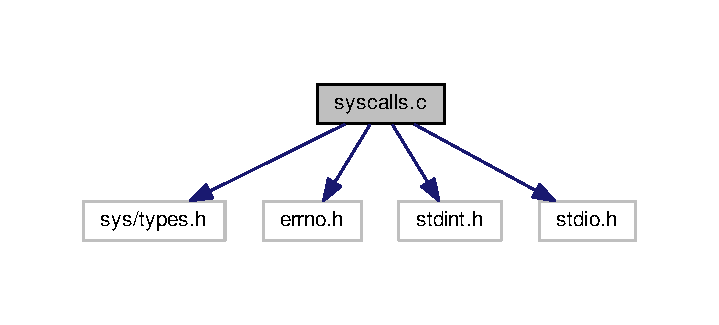
\includegraphics[width=345pt]{syscalls_8c__incl}
\end{center}
\end{figure}
\subsection*{Macros}
\begin{DoxyCompactItemize}
\item 
\hypertarget{group__newlib_gad72dbcf6d0153db1b8d8a58001feed83}{\#define {\bfseries D\+E\+B\+U\+G}~0}\label{group__newlib_gad72dbcf6d0153db1b8d8a58001feed83}

\item 
\hypertarget{group__newlib_ga1f464e950a4fa11e8821b5c725921a15}{\#define {\bfseries P\+R\+I\+N\+T\+F}(...)}\label{group__newlib_ga1f464e950a4fa11e8821b5c725921a15}

\end{DoxyCompactItemize}
\subsection*{Funções}
\begin{DoxyCompactItemize}
\item 
caddr\+\_\+t \hyperlink{group__newlib_gaae54d7b9578ba1fc171ce6f30f4c68a3}{\+\_\+sbrk} (int incr)
\begin{DoxyCompactList}\small\item\em Enlarges the allocated heap space. \end{DoxyCompactList}\end{DoxyCompactItemize}


\subsection{Descrição detalhada}
System calls. 


%--- End generated contents ---

% Index
\newpage
\phantomsection
\addcontentsline{toc}{chapter}{Índice}
\printindex

\end{document}
